% !Mode:: "TeX:UTF-8"
\documentclass[14pt,a4paper]{extreport}
\usepackage{cmap}

\usepackage{fix-cm}
%\usepackage[cp1251]{inputenc}
\usepackage[utf8]{inputenx}
\usepackage[russian]{babel}
%\usepackage{pscyr}
%\usepackage[T1]{fontenc} %cm-super
%\usepackage{type1cm}
\usepackage{indentfirst}

\usepackage{ifpdf}

\ifpdf
% we are running pdflatex, so convert .eps files to .pdf
\usepackage[pdftex]{graphicx}
\usepackage{epstopdf}
\else
% we are running LaTeX, not pdflatex
\usepackage{graphicx}
\fi


\usepackage{amsthm}
\usepackage{amssymb}
\usepackage{amsmath}
\usepackage{dsfont}
\usepackage{lscape}
\usepackage{makecell}
\usepackage{multirow}
\usepackage{hhline}
\usepackage{xspace}
\usepackage{ifthen}
\usepackage[numbers,compress,sort]{natbib}
\usepackage{setspace} % интервалы межстрочные
\pagestyle{plain} \setstretch{1.25} %1.3 = \onehalfspacing,  1.6 = \doublespacing

\usepackage[left=3cm,right=1.2cm,
top=2cm,bottom=2.5cm,bindingoffset=0cm,  %a4paper
]{geometry} % поля

%\textheight 25.7cm % 29.7-2-2
%\textwidth 16.7cm % 21-2.5-1.5
%\hoffset 0.46cm %2.5-2.54 слева 3 см
%\voffset -0.54cm %2-2.54 сверху 2 см
%\oddsidemargin 0cm \headheight 0cm \headsep 0cm \topmargin 0cm

\usepackage{ccaption} % заменяем для рисунков ':' после номера рисунка на другой символ
\captiondelim{. } % разделитель точка и пробел

\usepackage{listingsutf8}
\lstloadlanguages{RSL}
\lstset{%numbers=left,
language=RSL, extendedchars=true}
%, inputencoding=utf8/latin1, commentstyle=\itshape, stringstyle=\bfseries}


\newtheorem{theorem}{Теорема}
\newtheorem{lemma}{Лемма}
\newtheorem{utv}{Утверждение}
\newtheorem*{sld}{Следствие}


\newcommand{\LRU}{\textsf{LRU}\xspace}
\newcommand{\FIFO}{\textsf{FIFO}\xspace}
\newcommand{\PseudoLRU}{\textsf{Pseudo-LRU}\xspace}
\newcommand{\MRU}{\textsf{MRU}\xspace}

\newcommand{\lemmatext}[2]{
\noindent\textbf{Лемма~{#1}}. \textit{#2}
}

\newcommand{\theoremtext}[2]{
\noindent\textbf{Теорема~{#1}}. \textit{#2}
}

\newcommand{\theoremtextwname}[3]{
\noindent\textbf{Теорема~{#1}}~(#2). \textit{#3}
}

%
% Подправим команду \appendix : нумерация русскими буквами,
% а не латинскими.
\makeatletter
\renewcommand\appendix{\par
  \setcounter{chapter}{0}%
  \setcounter{section}{0}%
  \def\@chapapp{\appendixname}%
  \def\thechapter{\@Asbuk\c@chapter}}
\makeatother

% Теперь "русифицируем" окружение enumerate:
\makeatletter
\def\labelenumi{\theenumi)}      % чтобы после номера шла скобка;
\def\theenumii{\@asbuk\c@enumii}   % чтобы на втором уровне шли русские,
\def\labelenumii{\theenumii)}    % а не латинские буквы
\def\p@enumii{\theenumi}         % а это для \ref
\def\labelenumiii{{\bf--}}       % а на третьем уровне пусть будут лишь тире,
\let\theenumiii\relax            % и отдельных ссылок на него не будет
\def\p@enumiii{\theenumi\theenumii}
\makeatother

% !Mode:: "TeX:UTF-8"
\newcommand{\ccite}[1]{%
\ifthenelse{\isundefined{\nocites}}{\cite{#1}}{}%
}

\newcommand{\Actuality}{%
Современные микропроцессоры --- сложные многокомпонентные системы. Размеры современных микропроцессоров оцениваются как $10^7-10^8$ вентилей\ccite{HennesyPatterson}. Естественно при разработке таких сложных систем в проекты микропроцессоров вносятся ошибки, порой довольно критичные\ccite{IntelValidation}. Поэтому для обнаружения этих ошибок в цикл разработки микропроцессора в обязательном порядке входят этапы функциональной верификации.

Чем позднее будут обнаружены ошибки в микропроцессорах, тем дороже обойдётся исправление ошибок: сделать это в готовой микросхеме, тем более выпущенной на рынок, практически невозможно. Тем актуальнее становятся методы обнаружения ошибок на ранних этапах разработки микропроцессоров. Цикл разработки предполагает подготовку микропроцессоров в виде исполнимых программных моделей на языках Verilog или VHDL\ccite{VHDL}. Это делает возможным проведение функциональной верификации на таких моделях (т.е. до производства самих микропроцессоров) и актуальным исследование методов такой верификации. Целью функциональной верификации программных моделей микропроцессоров является обнаружение ошибок реализации функциональности в программных моделях микропроцессоров.

Выделяют следующие виды функциональной верификации: экспертизу, имитационное тестирование и формальную верификацию\ccite{KamkinPopular}. Экспертиза предполагает анализ текстов моделей экспертами с целью оценки их корректности и обнаружения ошибок. Этот вид функциональной верификации эффективно применяется на ранних стадиях разработки. Однако ввиду наличия человеческого фактора после экспертизы ошибки в микропроцессоре всё же остаются. Методы формальной верификации позволяют дать исчерпывающий ответ на вопрос о корректности отдельных модулей и всего микропроцессора. Однако трудоемкость формальной верификации чрезвычайно велика. Например, при разработке Intel Pentium 4 были формально верифицированы модуль работы с плавающей точкой (FPU), модуль декодирования инструкции и логика внеочередного выполнения (out-of-order), было найдено порядка 20 новых ошибок, однако трудоемкость этого проекта составила порядка 60 человеко-лет\ccite{IntelValidation}.

Имитационное тестирование позволяет ценой меньших усилий обнаружить значительную часть ошибок, в том числе критичных ошибок. Имитационное тестирование проводят для отдельных модулей (тогда оно называется \emph{модульным тестированием}) и для всего микропроцессора в целом (тогда оно называется \emph{системным тестированием})\ccite{EDAbook}. Модули тестируются подачей на их входы специальных сигналов (\emph{модульных тестов}) со снятием выходных сигналов и последующим анализом выходных сигналов. Входом при системном тестировании являются программы на машинном языке (\emph{тестовые программы}). Проведение модульного тестирования требует кроме подготовки самих входных данных еще и подготовку тестирующей установки (testbench), выделение тестируемого модуля из всего проекта микропроцессора и т.п. Системное тестирование избавлено от этой необходимости. Поскольку размер и сложность отдельного модуля всегда меньше размера и сложности микропроцессора в целом, потенциально качество модульного тестирования может быть выше, чем системного. Однако для достижения высокого качества тестирования как число модульных тестов, так и совокупная трудоемкость их изготовления, получаются очень большими. Это вынуждает часть проверок проводить на модульном уровне, а другую часть на системном. Невысокая стоимость подготовки и проведения системного тестирования определила его наибольшую востребованность среди других методов функциональной верификации. Практически все разработчики микропроцессоров проводят системное тестирование.

Ключевым вопросом, определяющим качество тестирования, является вопрос выбора тестовых программ. Поскольку современные микропроцессоры обладают множеством инструкций (порядка сотен), длины конвейеров имеют порядок десятка стадий, количество различных состояний и ситуаций, в которых надо протестировать микропроцессор, измеряется десятками тысяч. Поэтому для тщательного системного тестирования нужно подобное же и количество тестовых программ. Это определяет актуальность задачи автоматического построения тестовых программ для системного тестирования.

Сложность микропроцессоров растет (увеличивается количество функциональных требований, количество ситуаций, в которых поведение микропроцессора должно обладать заданной спецификой). Это требует тестовых программ для проверки функциональных требований, которые не проверяются имеющимися тестовыми программами, и делает актуальными дальнейшие исследования в области построения тестов.

%%%%! подредактировать про "новое качество" - это непонятно.

К числу наиболее сложных механизмов современных процессоров (поэтому наиболее подверженных ошибкам), использующих конвейеры и многоуровневые буферы типа кэш-памяти, относится механизм доступа к памяти. Поэтому актуальной является задача построения тестовых программ для проверки подсистем управления (механизмами) памяти микропроцессоров.

%%%% тем более, что зачастую нет способов прямого создания ситуаций?

%%% нацеленные методы (итерация-фильтрация, прямые конструкторы, random expansion, csp) - систематичные
%%% ненацеленные методы не тестируют тщательно или не находят ошибки, если микропроцессор не сырой

%%% в обзоре про MMU добавить классификацию ситуаций, которые надо тестировать

%%% цели:
%%% 1) понять, какие тесты "хорошие" (определение)
%%% 2) проанализировать методы их получения
%%% 3) предложить улучшения с целью получения более качественных тестов

%%% NB: ситуации не обязательно задавать шаблонами

%%% в приложение поместить примеры описаний MIPS'овских инструкций в xml ?


%А) микропроцессоры сложные -> в них есть ошибки
%Современные микропроцессоры --- это сложные системы, поэтому вероятность появления ошибки как при проектировании микропроцессора, так и при его производстве становится всё выше. При этом <<цена ошибки>> в готовом микропроцессоре велика (как минимум, это означает перевыпуск микропроцессора заново). Поэтому актуально развитие методов верификации микропроцессоров.

%%В) основная доля ошибок на этапе разработки моделей (design'а)
%Современные технологии проектирования микропроцессоров представляют собой средства разработки \emph{модели (design) на специальных языках} типа VHDL или Verilog~\cite{VerilogDesign}. Эти технологии позволяют в конечном итоге построить так называемые <<синтезируемые модели>>, из которых автоматически получаются фотошаблоны, необходимые для производства. Основная доля ошибок появляется именно на этапе разработки моделей (design), поэтому основные усилия по их выявлению или даже предотвращению их появления, также приходятся на фазу разработки моделей. Поэтому данная работа также нацелена на выявление ошибок в моделях микропроцессоров.

%%Г) модульное и системное тестирование ->
%% интересные ситуации нельзя создать инструкциями
%Тестирование на модели бывает \emph{модульным} (unit-level verification) и \emph{системным} (core-level verification, full-chip level verification)~\cite{UnitCoreLevel}. Модульное тестирование модели микропроцессора предполагает генерацию тестовых воздействий на входы отдельных модулей, блоков, микропроцессора, описанных на одном из языков типа VHDL, Verilog, и проверку выходов таких блоков. В рамках системного тестирования проверяется работа всего микропроцессора в целом --- тестом здесь является некоторая тестовая программа (программа на машинном языке), которая загружается в память и выполняется микропроцессором (речь все время идет о некоторой программной модели микропроцессора). Поскольку размер и сложность отдельного блока всегда меньше, размера и сложности микропроцессора в целом, потенциально качество модульного тестирования может быть выше, чем системного. Однако для достижения высокого качества тестирования как число модульных тестов, так и совокупная трудоемкость их изготовления, являются очень большими. Это вынуждает часть проверок проводить на модульном уровне, а другую часть на системном.

%Сложность микропроцессора определяет количество системных тестов. Если выделить различные аспекты функционирования микропроцессора (конвейер, буферы подсистемы управления памяти), то особое функционирование возникает при различных комбинациях этих аспектов. Это означает, что количество тестов должно быть не меньше произведения количества разных аспектов. Количество инструкций измеряется сотнями, а цепочек инструкций, соответственно, порядками сотен, плюс если учесть возможные аспекты в конвейере, в кэш-памяти, количество тестов получается очень большим. Для избежания проблемы такого <<взрывного>> характера количества тестов, их объединяют в классы эквивалентности --- \emph{тестовые ситуации}.

%При этом есть проблема покрытия всех потенциально интересных тестовых ситуаций. Нет никаких прямых способов создать многие из таких ситуаций нет. Например, интересно, как происходит доступ в память, когда соответствующий адрес имеется в кэш-памяти или не имеется. Или еще более тонкий анализ --- адрес имеется/или не имеется в кэш-памяти второго уровня. Среди инструкций процессора нет таких, которые были бы предназначены специально для создания таких ситуаций. Эти ситуации создаются \emph{динамически} в ходе выполнения программ.


%%Д) схема системного тестирования, показать здесь смежные вопросы
%% (вопросы построения оракула, покрытия и др.)
%Рассмотрим традиционную схему системного тестирования, известные подходы к автоматизации построения тестов и выявим проблемы, которые мешают строить более эффективные тесты.

%Микропроцессор рассматривается как черный (или серый) ящик. Входными тестовыми данными является некоторая программа, которая загружается в память. Результатом прогона теста является либо финальное состояние памяти (возможно, включая состояние регистров) или (в случае <<серого ящика>>) трасса изменения значений ячеек памяти или регистров.
%В этой общей схеме тестирования пока не упомянуты:
%\begin{itemize}
%	\item	генератор тестов (или набор уже готовых тестов);
%	\item	подсистема проверки корректности полученного результата --- тестового оракула, или арбитра;
%	\item	перечень <<интересных>> ситуаций, которые надо воспроизвести в ходе выполнения тестов;
%	\item	некая система мониторинга, которая фиксирует прохождение <<интересных>> ситуаций --- оценивает полноту покрытия.
%\end{itemize}
%
%Тестовый оракул, или арбитр, строится по схеме с использованием <<эталонной>> модели (simulation-based verification)~\cite{SimulationBased}. Каждая тестовая программа выполняется на двух моделях --- на тестируемой (design) и на <<эталонной>>. Потом состояния памяти или трассы изменения состояния памяти для тестируемой и эталонной моделей сравниваются. Если оракул признает, что трассы не эквивалентны, это свидетельствует о наличии ошибки в тестируемой системе (или эталонной, но это происходит реже). Как правило, эталонная модель пишется на одном из языков программирования (например, Си или Си++) и не загромождается деталями.  На этом основании считается, что такая модель существенно проще тестируемой, в ней с меньшей вероятностью встречаются ошибки, именно поэтому к ней можно относиться как к <<эталонной>>.
%
%% критика этого подхода: он не позволяет проверить модули, работающие за счет внешних воздействий - For example, fast interrupt request (FIQ), interrupt request (IRQ), data abort exception (Dabort) and prefetch abort exception (Pabort) of ARM7. Это пишут в статье "Automatic Verification of External Interrupt Behaviors for Microprocessor Design", авторы Fu-Ching Yang, Wen-Kai Huang, Ing-Jer Huang.
%
%
%Методы автоматической генерации тестов делят на псевдослучайные/комбинаторные (pseudo-random) и целенаправленные (что не отменяет возможности использования уже готовых тестов)~\cite{HoPhD}. В случае псевдослучайной генерации инструкции, их порядок и аргументы выбираются случайным образом или перебираются некоторым комбинаторным способом. Целенаправленная генерация начинается с задания некоторого шаблона тестовой программы, который определяет набор инструкций, их последовательность и аргументы. В рамках целенаправленной генерации порядок инструкций и их аргументы должны быть подобраны таким образом, чтобы каждый новый тест покрывал новые, еще не покрытые тестовые ситуации. Целенаправленную генерацию можно реализовать как выполнение массовой генерации комбинаторных тестов с последующей фильтрацией, с тем чтобы оставлять только те тесты, которые дают дополнительное покрытие. Однако уже для достаточно коротких шаблонов (длиной 3-4 инструкции) перебор становится слишком большим.
%
%Целенаправленная генерация тестов дает по тесту на каждую ситуацию. Набор тестов, которые покрывают все ситуации, называют нацеленными тестами (нацеленными на эти ситуации). Набор ситуаций конечен, следовательно и набор нацеленных тестов конечен. Вопрос
%%(это и есть основная тема исследования)
%, как систематическим образом строить тестовые программы, чтобы в совокупности они воспроизвели все заданные <<интересные>> ситуации.
%
%
%Перечень (конечный) <<интересных>> ситуаций и мониторинг. В совокупности две эти возможности задают метрику и механизм оценки полноты тестирования. Мониторинг организовать относительно легко, поскольку мы работаем не с реальным процессором, а с его моделями. Как построить перечень «интересных» ситуаций» --- вопрос открытый --- это одно из направлений моей работы.
%
%%Е) нацеленное/ненацеленное тестирование
}

%%%%%%%%%%%%%%%%%%%%%%
%%%%%%%%%%%%%%%%%%%%%%
%%%%%%%%%%%%%%%%%%%%%%


\newcommand{\Objective}{%
%Ж) формулирование цели работы - исследование методов построения нацеленных тестов-программ (на память)
%Целью исследования является разработка методов целенаправленной генерации системных тестов, которые, в свою очередь, должны предлагать и адекватные методы задания метрики и оценки полноты покрытия в соответствии с предложенными метриками.

Целью диссертационной работы является исследование и разработка методов и программных средств построения тестовых программ для проверки подсистем управления памяти микропроцессоров.

%%% надо тут, видимо, более точно изложить цель - что целью является улучшение некоторых ппараметров!

Для достижения этой цели были поставлены следующие задачи:
\begin{enumerate}
	\item исследовать описанные в научной литературе методы построения тестовых программ на предмет их применимости для системного тестирования подсистем управления памяти микропроцессоров;
	\item разработать методы построения тестовых программ для системного функционального тестирования подсистем управления памяти.
\end{enumerate}
}

%%%%%%%%%%%%%%%%%%%%%%
%%%%%%%%%%%%%%%%%%%%%%
%%%%%%%%%%%%%%%%%%%%%%


\newcommand{\Novelty}{%

Научной новизной обладают следующие результаты работы:
\begin{enumerate}
    \item предложен подход к построению тестовых программ для проверки подсистем управления памяти микропроцессоров, сочетающий формализацию документации и технику ограничений;

    \item предложен метод моделирования устройств подсистемы управления памяти, использующий конечные автоматы специального вида;

    \item предложена формальная модель инструкций, описывающая отдельные пути их выполнения в виде утверждений о свойствах параметров инструкций и модельном состоянии устройств;

    \item в рамках предложенного подхода разработан метод формализации механизма вытеснения данных при помощи построения ограничений, эффективно разрешаемых современным инструментарием.
\end{enumerate}

}

%%%%%%%%%%%%%%%%%%%%%%
%%%%%%%%%%%%%%%%%%%%%%
%%%%%%%%%%%%%%%%%%%%%%


\newcommand{\PracticalValue}{%

Разработанные модели и методы могут быть использованы коллективами, занимающимися разработкой микропроцессоров, для автоматизации построения тестовых программ. Разработанный прототип системы построения тестовых программ использовался для генерации тестов подсистем управления памяти ряда микропроцессоров архитектуры MIPS64. Результаты работы могут быть использованы в исследованиях, которые ведутся в Институте системного программирования РАН, Московском государственном институте электроники и математики, НИИ системных исследований РАН, Институте точной механики и вычислительной техники им. С.А. Лебедева РАН, Институте проблем информатики РАН и других
научных и промышленных организациях.

}

%%%%%%%%%%%%%%%%%%%%%%
%%%%%%%%%%%%%%%%%%%%%%
%%%%%%%%%%%%%%%%%%%%%%

\newcommand{\Pub}{

По материалам диссертации опубликовано одиннадцать работ~\cite{my_syrcose_2008, my_isp_2008, my_lomonosov_2009, my_lomonosov_2010, my_miet_2009, my_nivc_2009, my_syrcose_2009, my_isp_2009, my_ewdts_2009, my_programmirovanie_2010, my_isp_2010}, в том числе одна~\cite{my_programmirovanie_2010} в издании, входящем в перечень ведущих рецензируемых научных журналов и изданий ВАК. Основные положения докладывались на следующих конференциях и семинарах:
\begin{enumerate}
  \item на втором и третьем весеннем коллоквиуме молодых исследователей в области программной инженерии (SYRCoSE) (2008 и 2009 гг.);
  \item на шестнадцатой и семнадцатой международной конференции студентов, аспирантов и молодых ученых <<Ломоносов>> (2009 и 2010 гг.);
  \item на шестнадцатой всероссийской межвузовской научно-технической конференции студентов и аспирантов <<Микроэлектроника и информатика - 2009>> (2009 г.);
  \item на седьмом международном симпозиуме по проектированию и тестированию под эгидой IEEE (EWDTS) (2009 г.);
  \item на российско-ирландской летней школе по научным вычислениям (2009 г.);
  \item на научной конференции <<Тихоновские чтения>> (2009 г.);
  \item на научной конференции <<Ломоносовские чтения>> (2010 г.);
  \item на объединенном научно-исследовательском семинаре имени М.Р. Шура-Бура (2010 г.);
  \item на семинаре Лаборатории вычислительных комплексов факультета вычислительной математики и кибернетики МГУ имени М.В.Ломоносова (2010 г.);
  \item на семинаре отдела Технологий программирования института системного программирования РАН (2009, 2010 гг.).
\end{enumerate}

}

%%%%%%%%%%%%%%%%%%%%%%
%%%%%%%%%%%%%%%%%%%%%%
%%%%%%%%%%%%%%%%%%%%%%


\newcommand{\Structure}{%Структура и объем диссертации

Работа состоит из введения, трех глав, заключения, списка литературы и приложений.
Общий объем основной части диссертации составляет 125 страниц.
Список литературы содержит 71 наименование.
}

\newcommand{\Results}{%
\begin{enumerate}
  \item	Предложен подход к построению тестовых программ для проверки подсистем управления памяти микропроцессоров, позволяющий понизить сложность построения некоторых классов тестовых программ. В таких тестовых программах имеется цепочка длиной от 6 до 12 инструкций обращения к памяти. Понижение сложности обосновано при помощи ряда экспериментов на прототипе программного средства построения тестовых программ. Теоретически обоснована корректность алгоритмов в рамках подхода к построения тестовых программ.

%  \item Предложен метод моделирования устройств подсистемы управления памяти, использующий расширенные конечные автоматы с заданным набором операций. Моделью состояния является последовательность ассоциативных массивов, операциями --- операции обращений в устройство при наличии искомого ключа в ассоциативных массивах и при его отсутствии.
%
%  \item Предложена модель инструкций для описания отдельных путей выполнения инструкций в виде набора утверждений о свойствах операндов инструкций и содержимого устройств и изменения содержимого устройств.
%
  \item В рамках предложенного подхода разработан метод моделирования механизма вытеснения данных, позволяющий в отличие от других методов моделирования выразить ряд свойств вытесняемых данных в виде ограничений, эффективно разрешаемых современным инструментарием. Теоретически обоснована корректность метода для ряда стратегий вытеснения.

%  \item На основе предложенных моделей и методов создан прототип системы построения тестовых программ для проверки подсистем управления памяти микропроцессоров архитектуры MIPS64 и проведены эксперименты для оценки эффективности разработанного прототипа.
\end{enumerate}
}


\begin{document}

\thispagestyle{empty}

\begin{singlespace}
\begin{center}
%МИНИСТЕРСТВО ОБРАЗОВАНИЯ И НАУКИ\\ РОССИЙСКОЙ ФЕДЕРАЦИИ\\[0.5cm]
%
МОСКОВСКИЙ ГОСУДАРСТВЕННЫЙ УНИВЕРСИТЕТ\\ ИМЕНИ М.~В.~ЛОМОНОСОВА\\[0.5cm]

ФАКУЛЬТЕТ ВЫЧИСЛИТЕЛЬНОЙ МАТЕМАТИКИ\\ И КИБЕРНЕТИКИ\\[1cm]
\end{center}

\begin{flushright}
На правах рукописи\\[2cm]
\end{flushright}

\begin{center}
Корныхин Евгений Валерьевич\\[1cm]
\textbf{%\renewcommand{\baselinestretch}{1.8}
%\fontsize{28pt}{50pt} \selectfont
\huge{\textsc{построение тестовых программ для проверки подсистем управления памяти микропроцессоров}}\\[0.5cm]}

Специальность 05.13.11 -- математическое и программное обеспечение вычислительных машин, комплексов и компьютерных сетей\\[1.5cm]


Диссертация на соискание ученой степени\\
кандидата физико-математических наук
\end{center}

\vspace{0.7cm}

\begin{flushright} Научный руководитель:\\
д.ф-м.н. Петренко Александр Константинович
\end{flushright}

\vspace{1.5cm}

\begin{center}
Москва -- 2010
\end{center}


\end{singlespace}

\pagebreak

\tableofcontents

%%! определение LRU не "на списках", а "на перестановках"! + аналогичные

%%! определиться "последовательность инициализирующих" или "инициализирующая посл-ть"

%% там, где в формулах разъехался "w-1", заменить на "w{-}1"

%%%%! не ВЕРШИНЫ АВТОМАТА, а СОСТОЯНИЯ ! не ДУГИ АВТОМАТА, а ПЕРЕХОДЫ !

%%? НУЖНЫ ЛИ ТОЧКИ ПОСЛЕ ЦИФР-НОМЕРОВ РАЗДЕЛОВ ?
%% http://fuzzy-plates.googlecode.com/svn-history/r68/trunk/docs/sty/russcorr.sty

%%%% 1. следить за числом и родом: "предлагаем" и "предлагается" - должен быть один вариант

% !Mode:: "TeX:UTF-8"
\newcommand{\LcurrentBody}{
Пусть $L_0$ -- множество ключей, расположенных в некотором регионе таблицы перед исполнением инструкций тестового шаблона, $x_1$, $x_2$, ..., $x_n$ -- последовательность ключей того же региона, по которым происходят обращения с промахами в том же порядке, что и в тестовом шаблоне, $x'_1, x'_2, ..., x'_n$ -- последовательность ключей, вытесняемых обращениями к $x_1$, $x_2$, ..., $x_n$. Тогда $L$ -- выражение для множества ключей таблицы того же региона после этих обращений имеет вид:
$$L \equiv L_0 \setminus \bigcup_{i=1}^n \{x'_i\} \cup \bigcup_{i=1}^n (
\{x_i\} \setminus \cup_{j~=~i+1}^n \{x'_j\}).$$
}

\newcommand{\HitMissEquations}{
Пусть $L_0$ -- множество ключей, расположенных в таблице в некотором регионе перед исполнением инструкций тестового шаблона, $x_1, x_2, ..., x_n$ -- последовательность ключей того же региона, по которым происходят обращения с промахами в том же порядке, что и в
тестовом шаблоне, $x'_1$, $x'_2$, ..., $x'_n$ -- последовательность ключей, вытесняемых обращениями к $x_1$, $x_2$, ..., $x_n$. Тогда для обращения после этих по ключу $x$ в тот же регион справедливы следующие уравнения:
\begin{itemize}
\item для обращения с попаданием:
$$
\left[
   \begin{array}{l}
    x \in L_0 \wedge x \notin \{x'_1, x'_2, ..., x'_n\} \\
    x = x_1 \wedge x \notin \{x'_2, ..., x'_n\} \\
    x = x_2 \wedge x \notin \{x'_3, ..., x'_n\} \\
    ...\\
    x = x_{n-1} \wedge x \notin \{x'_n\} \\
    x = x_n \\
   \end{array}
  \right.
$$

\item для обращения с промахом ($x'$ --- вытесняемый ключ):
$$
\left\{
   \begin{array}{l}

  \left[
   \begin{array}{l}
    x \notin L_0 \wedge x \notin \{x_1, x_2, ..., x_n\} \\
    x = x'_1 \wedge x \notin \{x_2, ..., x_n\} \\
    x = x'_2 \wedge x \notin \{x_3, ..., x_n\} \\
    ...\\
    x = x'_{n-1} \wedge x \notin \{x_n\} \\
    x = x'_n \\
   \end{array}
  \right. \\

  { }\\

  \left[
   \begin{array}{l}
    x' \in L_0 \wedge x \notin \{x'_1, x'_2, ..., x'_n\} \\
    x' = x_1 \wedge x \notin \{x'_2, ..., x'_n\} \\
    x' = x_2 \wedge x \notin \{x'_3, ..., x'_n\} \\
    ...\\
    x' = x_{n-1} \wedge x \notin \{x'_n\} \\
    x' = x_n \\
   \end{array}
  \right. \\

  { }\\

  displaced(x')\\

%  { }\\
%
%  R(x) = R(x')\\
%
  \end{array}
\right.
$$

\end{itemize}
}

\newcommand{\CorrectnessMirror}{
%Если тестовый шаблон является совместным (т.е. для него существует хотя бы одна тестовая программа), то тестовая программа (инициализация плюс инструкции тестового шаблона), построенная по предлагаемому методу, соответствует тестовому шаблону.
Если система ограничений, построенная для последовательности обращений к таблице $(S_1, k_1, R_1)$, $(S_2, k_2, R_2)$, ..., $(S_n, k_n, R_n)$ c дополнительным предикатом $P(k_1,$ $k_2, ..., k_n, R_1, R_2, ..., R_n)$, является совместной, то ее решение $t_1, t_2, ..., t_m$, $r_1$, $r_2$, ..., $r_m$, $k_1, k_2,$ ..., $k_n$, $R_1, R_2, ..., R_n$, удовлетворяет последовательности $S_1, ..., S_n$ и $P$ при любом начальном состоянии таблицы.
}

\newcommand{\FullnessMirror}{
Фиксируем некоторое начальное состояние $L$ таблицы со стратегией вытеснения не \texttt{none}. Если при нем для последовательности обращений к таблице $(S_1, k_1, R_1)$, $(S_2, k_2, R_2)$, ..., $(S_n, k_n, R_n)$ c дополнительным предикатом $P(k_1$, $k_2, ..., k_n, R_1$, $R_2, ..., R_n)$ существуют значения переменных $k_1,$ $k_2,$ ..., $k_n$ и $R_1$, $R_2, ..., R_n$, которые удовлетворяют последовательности $S_1, S_2, ..., S_n$ и $P$, то система ограничений, построенная согласно  алгоритму генерации ограничений на ключи обращений для таблицы со стратегией вытеснения не none,
%из раздела~\ref{sec:constraints_generation_section}
будет совместной, если стратегия вытеснения является <<существенно вытесняющей>>.
}

\newcommand{\FullnessMirrorNone}{
Фиксируем некоторое начальное состояние $L$ таблицы со стратегией вытеснения \texttt{none}. Если при нем для последовательности обращений к таблице $(S_1, k_1, R_1)$, $(S_2, k_2, R_2)$, ..., $(S_n, k_n, R_n)$ c дополнительным предикатом $P(k_1$, $k_2, ..., k_n, R_1$, $R_2, ..., R_n)$ существуют значения переменных $k_1, k_2, ..., k_n$ и $R_1$, $R_2, ..., R_n$, которые удовлетворяют последовательности $S_1, S_2, ..., S_n$ и $P$, то система ограничений, построенная согласно  алгоритму генерации ограничений на ключи обращений для таблицы со стратегией вытеснения none,
%из раздела~\ref{sec:constraints_generation_section}
 будет совместной.
}

\newcommand{\PseudoLRUEssential}{
Стратегия вытеснения \PseudoLRU является существенно вытесняющей.
}

\newcommand{\UpperBoundLRUMirror}{
Фиксируем некоторое начальное состояние $L$ таблицы со стратегией вытеснения \LRU. Если при нем для последовательности обращений к таблице $(S_1, k_1, R_1)$, $(S_2, k_2, R_2)$, ..., $(S_n, k_n, R_n)$ c дополнительным предикатом $P(k_1$, $k_2, ..., k_n, R_1$, $R_2, ..., R_n)$ существуют значения переменных $k_1, k_2, ..., k_n$ и $R_1$, $R_2, ..., R_n$, которые удовлетворяют последовательности $S_1, S_2, ..., S_n$ и $P$, то система ограничений, построенная согласно  алгоритму генерации ограничений на ключи обращений будет совместной для любого $m > n\cdot w + M$, где $M$ -- количество элементов последовательности $S_1, S_2, ..., S_n$, равных miss.}

\newcommand{\PseudoLRUInvariant}{
Пусть ($\alpha_1~\alpha_2~\dots~\alpha_W$)
--- \PseudoLRU-ветвь некоторой позиции $i$. Тогда изменение этой
ветви согласно стратегии вытеснения \PseudoLRU определяется только
относительной позицией (относительно $i$) и происходит следующим
образом при обращении к ключу с (абсолютной) позицией $j$: если
$\pi^i_j \in [\frac{w}{2^k},~\frac{w}{2^{k-1}})$ для некоторого
$k=1,2,\dots,W$, то происходит изменение $\alpha_1 := 0,~\alpha_2 :=
0,~\dots,~ \alpha_{k-1} := 0,~\alpha_k := 1$; если $\pi^i_j = 0$, то
происходит изменение $\alpha_1 := 0,~\alpha_2 := 0,~\dots,~\alpha_W
:= 0$; вытеснение ключа на позиции $i$ происходит в том случае, когда
$\alpha_1 = 1~\wedge~\alpha_2 = 1~\wedge~\dots~\wedge~\alpha_W = 1$.
}

%\newcommand{\DiapazonLRU}{
%Решение системы (ключ $x'$)
%$$
%\left\{
%   \begin{array}{l}
%    x' = y \\
%    R(y) \cap (L \setminus \{x_1, x_2, ..., x_n\} ) = \{y\}\\
%   \end{array}
%  \right.
%$$
%где последовательность ключей $y, x_1, x_2, ..., x_n$ -- диапазон
%вытеснения, а $L$ -- множество ключей в таблице перед концом
%диапазона, является вытесняемым ключом для стратегии вытеснения \LRU
%согласно определению на перестановках.
%}
%
%\newcommand{\DiapazonFIFO}{
%Решение системы (ключ $y'$)
%$$
%\left\{
%   \begin{array}{l}
%    y' = y \\
%    R(y) \cap (L \setminus \{y_1, y_2, ..., y_n\} ) = \{y\}\\
%   \end{array}
%  \right.
%$$
%где последовательность ключей $y, y_1, y_2, ..., y_n$ -- диапазон
%вытеснения, является вытесняемым ключом для стратегии вытеснения
%\FIFO согласно определению на перестановках.
%}
%
%\newcommand{\MaxUpperBoundLRU}{
%$$0 \leqslant k \leqslant n \cdot w_1$$
%$$0 \leqslant h \leqslant n \cdot (w_1 + w_2 + 2)$$
%где $w_1$ -- ассоциативность кэш-памяти первого уровня, $w_2$ --
%ассоциативность кэш-памяти второго уровня, $n$ -- количество
%инструкций тестового шаблона.
%}

\newcommand{\LRUusefuls}{
Пусть $(t_1, r_1)$, $(t_2,r_2),$ ..., $(t_m,r_m)$ -- ключи и регионы инициализирующих обращений, $(k_i, R_i)$ -- ключ и регион обращения, для которого описывается вытеснение (будем его называть <<вытесняемым>>), причем $(k_i||R_i) \in \{(t_1||r_1)$, ..., $(t_m||r_m)$, $(k_1||R_1)$, ..., $(k_{i-1}||R_{i-1})\}$ и $\{(t_1||r_1), ...,(t_m||r_m)\}$ --- все разные. Тогда $k_i$ не вытеснен из региона $R_i$ согласно определению \LRU на перестановках тогда и только тогда, когда $$\sum\limits_{j=1}^{m+n} [u_{k_i,R_i}(s_j)] < w$$
где последовательность $s \equiv \langle (t_1||r_1), ..., (t_m||r_m), (k_1||R_1), ..., (k_n||R_n)\rangle$,\\$R(s_i)$~---~вторая компонента $s_i$ (регион), а формула полезного обращения такая:
$$u_{k_i,R_i}(s_j) \equiv ((k_i||R_i) \notin \{s_j, ..., s_{m+n}\} \wedge
R_i = R(s_j) \wedge s_j \notin\{s_{j+1},..., s_{m+n}\})$$
}

\newcommand{\PLRUusefuls}{
Пусть $(t_1, r_1)$, $(t_2,r_2),$ ..., $(t_m,r_m)$ -- ключи и регионы инициализирующих обращений, а $(k_i, R_i)$ -- ключ и регион обращения, для которого описывается вытеснение (будем его называть <<вытесняемым>>), причем $(k_i||R_i) \in \{(t_1||r_1)$, ..., $(t_m||r_m)$, $(k_1||R_1)$, ..., $(k_{i-1}||R_{i-1})\}$ и $\{(t_1||r_1), ...,(t_m||r_m)\}$ --- все разные. Тогда $k$ не вытеснен из региона $R$ согласно трактовке \PseudoLRU в терминах ветвей бинарного дерева тогда и только тогда, когда $$\sum\limits_{j=1}^{m+n} [u_{k_i,R_i, \pi'_i}(s_j)] < W$$
где последовательность $s \equiv \langle (t_1||r_1), ..., (t_m||r_m), (k_1||R_1), ..., (k_n||R_n)\rangle$,\\$R(s_i)$ --- вторая компонента $s_i$ (регион), а формула полезного обращения такая:
$$u_{k_i,R_i,\pi'_i} (s_j) \equiv \left\{\begin{array}{l}
(k_i||R_i) \notin \{s_j, s_{j+1}, ..., s_{m+n}\}\\
R_i = R(s_j)\\
(\pi'_i||R_i) \in \{(\pi_j||R_j), (\pi_{j+1}||R_{j+1}), ..., (\pi_{m+n}||R_{m+n})\}\\
\bigwedge\limits_{k = j+1}^{m+n} (R_j = R_k ~\wedge~(\pi'_i||R_i) \notin \{(\pi_j||R_j), (\pi_{j+1}||R_{j+1}), ..., (\pi_k||R_k)\}\\
\hspace{2cm} \rightarrow P(\pi_j \oplus \pi'_i, \pi_k \oplus \pi'_i))\\
\end{array}\right.
$$
$$P(x, y) \equiv (y > x~~\wedge~~x \oplus y > x)$$

$\pi'_i$ определено следующим образом: если $S_i$ = hit, то
$$
\begin{array}{l}
\texttt{(ite~} ((k_i||R_i) = (k_{i-1}||R_{i-1})) ~~ (\pi'_i = \pi_{i-1})\\
\texttt{(ite~} ((k_i||R_i) = (k_{i-2}||R_{i-2})) ~~ (\pi'_i = \pi_{i-2})\\
... ~(\pi'_i = 0)\texttt{)))...)}\\
\end{array}
$$

если $S_i = $ miss, то ( $\{\pi_i, ..., \pi_j\}_m$ обозначает подмножество множества позиций от $i$'го до $j$'го обращения из неуспешных обращений):
$$
\begin{array}{l}
\texttt{(ite~} ((k_i||R_i) = (k_{i-1}||R_{i-1})) ~~ (\pi'_i = \pi_{i-1})\\
\texttt{(ite~} ((k_i||R_i) = (k_{i-2}||R_{i-2})) ~~ (\pi'_i = \pi_{i-2} \wedge \pi'_i \in \{\pi_{i-1}\}_m)\\
\texttt{(ite~} ((k_i||R_i) = (k_{i-3}||R_{i-3})) ~~ (\pi'_i = \pi_{i-3} \wedge \pi'_i \in \{\pi_{i-1}, \pi_{i-2}\}_m)\\
... ~(\pi'_i = 0)\texttt{)))...)}\\
\end{array}
$$
} 

\addcontentsline{toc}{chapter}{Введение}
\chapter*{Введение}

\section*{Актуальность}
\Actuality

\section*{Цель работы}
\Objective

\section*{Научная новизна}
\Novelty

\section*{Практическая значимость}
\PracticalValue

\section*{Публикации}
По материалам диссертации опубликовано одиннадцать работ~\cite{my_syrcose_2008, my_isp_2008, my_lomonosov_2009, my_lomonosov_2010, my_miet_2009, my_nivc_2009, my_syrcose_2009, my_isp_2009, my_ewdts_2009, my_programmirovanie_2010, my_isp_2010}, в том числе одна~\cite{my_programmirovanie_2010} в издании, входящем в перечень ведущих рецензируемых научных журналов и изданий ВАК.

\section*{Структура работы}
Первая глава посвящена обзору существующих методов построения тестовых программ и подсистем управления памяти, их анализу и уточнению задач исследования. Вторая глава посвящена решению сформулированных в конце первой главы задач. В этой главе описываются предлагаемые модели и методы для построения тестовых программ. Третья глава посвящена оценке применимости предлагаемых во второй главе моделей для существующих практически важных архитектур микропроцессоров, описанию реализации программного средства для генерации тестовых программ и проводившихся на этой реализации экспериментов с целью оценки качества предлагаемых во второй главе методов.

\section*{Об обозначениях}

Наиболее значимые утверждения помечены как <<Теоремы>>, доказательства большинства из них помещены в приложении~\ref{sec:proofs}. Менее значимые утверждения помечены как <<Утверждения>>. Обоснования <<Утверждений>> обычно представлены непосредственно перед формулировкой <<Утверждений>>. Вспомогательные утверждения помечены как <<Леммы>>.


\section{����� ����� �� ���������� ��������������� ������������
����������������}

� ��������� ����� � �������� ���������� ��������������� ������������
���������������� ����� �������� ��������� ������� � ����������
�������� ��������:
\begin{itemize}
\item \emph{������ ���������� �������� ��������} ���� � ����������� �����������
��� ������� ������������ ���������������, �� �� ����� �����������
��� ������������ ������, ������� �������;
\item \emph{������������ � �������������� �����-����������} ����������� �����
��-�� ��������� ��������� ��� ����������: ����� ������������
������������ ��������������� ����� �������� ������ �����-����������,
� ���, ��������������� ��� �����-����������, ��� �����. ������
������������� ������� ����� ������������ �� �����;
\item \emph{��������� ��������� �������� ��������} ����������� ��� �� ����� �
���� �������� �������������. ��������������� ����� ������� ��������
��������� ��������� ������ ���������� ������� ������, ������ ��
����������� ������� ������������. ��������������� � ����� �������
�������� ��������� ���������~\cite{muGP};
\item \emph{��������� �������� �������� �� ������ ��������
��������} ������������ ���������� �������� ��������� ��������
��������� �� ��� ����� (��. ���.~\ref{pic_commonprocess}): �� ������
���������������� �������� ������� -- ����������� �������������
�������� �������� (� �������� �������� ��� ���������� ����������
������ �������� ����������� ����������� �� ��������) -- � �� ������
����� �� �������� �������� ������������ �������� ���������. ������
���� �������� � ���� \emph{��������� �������� ������}, �.�.
��������� ���������� ���������� (����������-��������) � ���������
�������� ���������, ����� ���-������, ����� TLB � �.�. ������ �����
��������� ��� ���������� �������� � �������� �������, � ������ �����
��������� ����� ������� ��������� �������� ������.
\end{itemize}

\begin{figure}
\center
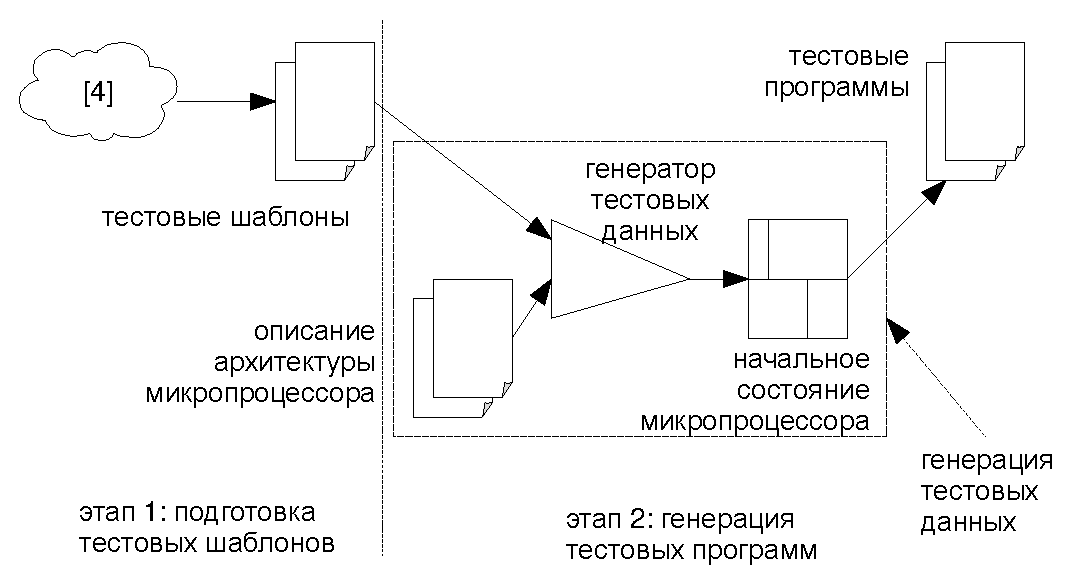
\includegraphics[width=0.8\textwidth]{test.eps}
\caption{��������� �������� �������� �� ������ ��������
��������}\label{pic_commonprocess}
\end{figure}

�������� ������� ��������� ������������������ ����������, ���������
���������� � ��������� ������������ ������� (��������, ������������,
������� ��� ��������� � ���-������). � �������� ����������
���������� ����� ���� ��� ���� ������� �������� � ���������, ��� �
������������� ����������� ����������� ������ ��������� ��������.
������������������ ���������� ���� ����� ������ ����. �������������
� �������� ������� ������ ��������� �����, ����� ������������
���������� ���������� ������� � ��� ���� ��������
������������������� ����������, ������ �� ������� ������ ����
��������� �������� �������. ������ ��������� �������:

{ \normalsize
\begin{verbatim}
REGISTER ax:32;
REGISTER bx:32;
REGISTER cx:32;
LW cx, ax, 0 @ l1Hit
SD ax, bx, 2 @ l1Miss
\end{verbatim}
}

\noindent � ���� �������� ������� 2 ���������� -- LW � SD. � ������
���������� ������� ��������� -- 2 �������� � ��������� -- � �����
����� '@' ���������� � ���, ��� ������ ���� ��������� ����������
(����������� �� �������� ���������� ���������� � ���������
���������������): l1Hit -- c ���-���������� (��� �������� �� ������
������ �� ���������� ����������� ������ � ������ ����������
���������� ������ �������������� � ���-������) � l1Miss -- c
���-�������� (��� �������� �� ������ ������ �� ����������
����������� ������ � ������ ���������� ���������� �� ������
�������������� � ���-������). ����� �������� �������� ��������� ��
����� �������, ���������� ������ ��������� �������� ��������� ax, bx
� cx � ��� ����� ���-������, � ������� �������� ����������
 -- ��� � ����� �������� ������ ��� ������� �������. ��� �����
�������, ������� � ������ ��������� ������� ���������� �������������
��������� ���������������. ���������� �������� ��������� �����
��������� � ���������, ��������� �� ��������� ������ ���������� �
���, ��� ���� �������� � �������� �������.

��������� � ������ ��������� �������� ������. ����� ��������� �����
����� �������� ��������� ������ �� �������:
\begin{itemize}
\item ������������� �������;
\item ������� ������ ATPG;
\item ���������� �����������.
\end{itemize}

\emph{������������� �������} ��������� � ������ ������� ��������
��������. ����� �������� ������� �������� ���� ������� �����������,
� ������ �������� ������� �������� ����������. ������ ��� ��������
���� ������� � �������� ��������� �����������. ������� ���� �
�������, �� �������� ������������ � ����������, ��������� �� ������
���������� �������� ����������� �� ���������� � ������ ��������
����. � ������ �������������� �� Fujitsu Lab.~\cite{TSE}
������������ ������� �������� ��������� � ���� ��������� (Test
Specification Expressions, TSE), � ���������� ��������������� -- ��
����� ISDL. ����������� ��������� ������ �������� ���������,
��������������� TSE. Kohno � Matsumoto~\cite{mVpGen} �������������
������ ����������� ����������� ����������������, ��������� ��� �����
��������� �������� �������� � ������� �������� ��������. �������
�������� ���������� � ����� �������� ������������ �� ��������� �
�������� ��������.

������������� �� Politecnico di Milano~\cite{toATPG} ����������
���������� �������� ������ � �������������� \emph{������ �������
������ ATPG} (Automatic Test Pattern Generation). ATPG -- ������
������ �������� ������� �������� (<<��������>>) ����� � ����� ������
�� ������������� ���������. ATPG ���� ����������� ��� ����������
������������, ���� �������� RTL-������ ���������������. ������ ATPG
�������� ����� � ��� �� ������� ���������� (� ��� �����
������������) �����������. ��� ���������� ATPG ��� ���������
�������� �������� ����������, ����� RTL-������ ��������������� ����
������ � ������� ��������� �������� ������. ����� ����,
������������� ����� �������� ������ ��� ��������������� ������������
����������, ��������� �������� ���������� �������������� �������
��������� ���������� -- ������� RTL-������ �������� ������,
�������������� ����������� � ��������� � ������� ��������������
����������� �� ���� ����������.

�������� ������������ ����������� ��������� �����������, ������������ ���
��������� �������� ������ \emph{���������� �����������}. ����������� �
���������� ����� ������ �� ��, ��� � ��������, � ������ ���������� �����������
-- �� ��, ��� � ������ ������������ ������� ����������, �� ��� ������� ����
������ ����������� ����������� ���������~\cite{ConstrProp}. �
������~\cite{MAATG} �������������� �� ���������� ������������� ������������
���������� ������������ ����������� ���������� MAATG. �������� ������ ��� ����
����� ��������� ���� ����������� ��������� ��� ����������� �������� � ��������
������� �������� ����������. ��� ������� ����������� ���������������
������������ �������� �� ����� EXPRESSION. ������ ���������� --
Genesys-Pro~\cite{GenesysPro2004} -- ��������������� ��������� IBM ���
����������, ��������� ������ �� ���������� ��������� 20 ���. �������� �������
��������� �������� �������� ��������� ���������� �����. ��� ����� ���������� �
�������� ������� ����� ���� ������� ��������� ��� ������ ��������
����������~\cite{GenesysPro2004Innovations}. ����� ��������� �������� ���� �
��������� �� ������� � ���-������ � ��� ���������� �������. ������ � ���������
������� �� ������������ ���������� ����� ��������, ��� �� ���� �����������
������ ������������� ��������� ��������, ���������� �� ������������ ������.
������� ������ ��������������� ������ ���� ������� � ���� �����������
(constraint net) �� ��������, ��� ��������, ��� �� �������� ������������
��������� ��������� ����������, �������� ���� � ������ ��� �����������
��������� ���������������� ���������� �� ������ ���������� ����������. ���
��������� ���������� ��������� ���������� Genesys-Pro ���������� ���
����������� �������� ��������� � ��������� ���������������, ������� ��������
���������. ���� ������ ��������� ���������������� �� ������� �������� �������,
�� � ������ � ������������� ������������� ��������� �������� (backtracking),
���� ������� ��������� ��� ��������� ���������� ����������.

%����� ���� ���������� �� ���������� """�������������� �����"""
%������ ������, � ���������� �������� ���������� ��������� �������,
%������ �� ��� ����������� ����� �������� ��������� �� ���� �������.
%����� �������, �������� ��������� �������� ��-��������, ��� �����
%������������ ��������� �� ������������� ������ Genesys-Pro ��
%������� �������� ��������.

% �� �������� ����� Genesys-Pro ���� ������ ��������� ��������� �������,
% � � ������ ����� ������� ������ - ����� ���������� ������������� �
% ��������� ���������! � IBM ��������� ������: ����� ������� - ���������
% ��������� ��� �������� (� �.�. ��� ����), � ��������� ������ "��������".
% ��������: cache = [ set1:0,5,10; set2:2,4,7 ], select(set,tag: cache miss)
% -> ������: set isin {1,2}, tag ~isin cache(set). ������ ������� ������ ��������,
% ����� ������. �������� set = 1, tag = 1. �� ������.
% � �������� ��� � ���, ��� � ����: (set,tag): cache miss,.... � ���!
% ��� ���� �������, ��� ����� miss.

� ������ ������ ��� ������� ������ ��������� �������� ������ �����
������������ ���������� �����������. ����������� ��� ������ � ������
��������������� ������� ���������� �������� �������� �� ������
������ ���������������~\cite{kamkin}. ������ ��� �������� ��������,
���������� � ������ ���� ��������������� �������, ���������� MAATG
����������, ��������� ������� ����� ��������� �� ������ �����������
��������� ��� ����������� ���������, �� � ����� ������� �����������,
��������, ���-������. � ������ ������ �� ��������� � Genesys-Pro
�������� ������ ������������� � ����������� ������� (��������, ���
������ ���������� ����������� (�.�. ������ ������������) NP-�����;
��� ��������, ��� ��� ������� �������� �������� ������������ �
������ ������ ����� ����� ���� �� ����� �����������, ������ ��������
����������, ��� ������ � ����������� ������ �������������� ��
�������� ���������� ��������� �����). ��� ������������ �����������
���������� ����������� �������� ������������� � ��������� ��������.
��-�� ����� ����������� �������� ����������� ������� �����������
(Genesys-Pro ������ ����� ������ � ��������� �����, �� �������
������� ���������). ����� ����, � ������ ������ ������������ �����
������������� ����� ���������� �������� ������: ������ ����������
��������������� ����� ���� �������� �� ��������� �����������
���������������.

������������ �������� ��������, ���������� � ������~\cite{kamkin}, ��������
�������� ��� ������ ���������� ���������-����������. ��� ����� ��������
Genesys-Pro ����� �������� ������ ������������, ��������� �������� �����������
� ������� ������ ���������� <<���������>> ���������� ��������� ���������� ���
�������� � �������� ������� ��� ��� �������. �� �������� ��������
��~\cite{kamkin} Genesys-Pro ����� �������� ��������� �������: �������
��������� ��������� ��������� ���������������, ������ ��������� �������� ������
(��������� ��������� ��������� ��� ��������), �� ��� ������ ������ ��
����������, ������� ����� ��������� �� ���, ��� ��������� � �������,
Genesys-Pro ������� ������� � ����� ������, � ������ ��� �������� �������
������ ��������� ��������� ��������������� � ���� ������� ��������� ������.
����� ������� ��������� �������� ������ ������� ������������. ��� ������� �����
���������� ������� � Genesys-Pro ������������ ������������ ������
DeepTrans~\cite{DeepTrans}. ������ �� ��������� ������� ���������� �������
����� � ���, ��� ����� ����� ���������� ������� ������������ � �����������.
������ ������ ���������� ��� �������� ������� ���������� ������ ��������
������� Memory � ������������ ���������. ��������, ��� ������� ����������
�����������, ����������� ������ � ���������� ������� ��� ����������� ��������,
�������� � ����� ������� ������������, ������������ ������� �� ���������� �����
����� ��������� ��� ��������.

������� �������� �������� ���� �� �������������� � ������ ������������
(����������� ��������� ��������� ������� �������� � ������������ ����� ���� �
���� �����������) ��� ���������� ������ � ������� �������� � ����� �������
������������, ������� �� ������� ��������� �� ���������� �����. ���� ��� �����
���������� ������� ��� ����������� ��������� ��������������� ����� ������������
������� ������ ������� ������� ������ ($mem_0 = var0 \wedge mem_1 = var1 \wedge
...$); ������ ��������� ������������ �� ������������ �������, ������� ���
������ ������ ��������� ��������������� ���������� ���������� ��� ���������
�������� ($mem[i] := x$ �������� � ������� $(i = 0 \wedge mem_0 = x \wedge
mem_1 = var1 \wedge ...) \vee (i = 1 \wedge mem_0 = var0 \wedge mem_1 = x
\wedge ...) \vee ...$), � ���� ����� ��������� ���������, �� ����������
������������� ��� ��������� �������� �������� ��������. ������������ �������
����� ������ ������� $|L| \cdot 2^n$, ��� $|L|$ -- ������ ������, � $n$ --
���������� ��������� ������. � ������ ������ ��������� ����� �����������
���������, ���������� � ������� ������� ������� $|L| + n$.

% ������� �� Genesys-Pro:
% 1) ������ �������� ��������� ��������� �������:
%    �������� ������ ��������������� �������, � �� �� ����� �������
% 2) ������ ���������� �������� ������ (��������, ���������� ���������)
%    �������� ����� �������. Genesys-Pro �� ���� ��, � �������� ������ �����
%    ������. ���� ������ �������, �����. � � ���� ������ �����.
% 3) ������������ ����� �������� �������� �������� ��������.
%    �� �����������, � ���������.
% 4) ���� ��������� ��������� ������ �������� ��������, ��������� ��� ���
%    ������� � ������������ �� �������� ����������� :)
% 5) Genesys-Pro �� �������� ��������, ��� ��� ����������� ���-�� ���������
%   (���, ��������, � ������� ��������), ����� �������� ������ ������������,
%   ��� ������������� ������ Genesys-Pro ����������� � �� ���� ����, ��� �� ���
%   ����� �������� ���������, ��������, ��������, ���� � ������� ��� ��������,
%   ����� ��� ������ ���� �������. �� ������� �������� Genesys-Pro �����������
%   ��������� ��������� ��������� ���������������, � ����� ������ ������ ���������
%   ������ (��������� � ������� �������� ��� �������� ��� �������). ����� ��������
%   �������� �������� - �� ���� ����� ������� Genesys-Pro. � ��� ���� ��� ����������
%   ��������� ������� �� ���������� ��������� �������� ��������, Genesys-Pro
%   ��������� � ������ ������ � ������� ������ ��������� ���������. ����� ��������
%   �������� ������. ���� �� ����������, ����� ������� � ����� ������ ���������� ��������.
%   ����� ����� ������������ � ����� ���������� ������!


% !Mode:: "TeX:UTF-8"

\newcommand{\cmpn}[1]{\textsf{#1}}

\chapter{Описание предлагаемых методов и моделей}

\section{Описание предлагаемого подхода генерации тестовых программ}\label{sec:approach}

Рассмотрим следующую схему предлагаемого программного средства для генерации тестовой программы по тестовому шаблону (рисунок~\ref{fig:gen_scheme}). Программное средство изображено на схеме прямоугольником с подчеркнутыми границами. Внутри прямоугольника расположено 2 других прямоугольника, означающих следующие компоненты программного средства: \cmpn{Генератор ограничений} и \cmpn{Конструктор текстов программ}. На схеме есть прямоугольник \cmpn{Решатель ограничений} --- это другое программное средство, внешнее к программному средству для генерации тестовой программы. Остальные элементы схемы --- это исходные и выходные текстовые данные (тестовый шаблон, описания вариантов исполнения инструкций, описания устройств подсистемы управления памяти и тестовая программа), параллелограмм означает, что программное средство для генерации тестовой программы определило невозможность построения тестовой программы для данных исходных текстовых данных. Стрелки от текстовых данных к компонентам программного средства означают то, что эти текстовые данные являются входом компонентов. Стрелка от компонента \cmpn{Конструктор текстов программ} к тестовой программе означает то, что этот компонент строит тестовую программу. Стрелка от компонента \cmpn{Генератор ограничений} к \cmpn{Решатель ограничений}, подписанная словом <<ограничения>>, означает, что \cmpn{Генератор ограничений} строит ограничения, которые передаются как вход \cmpn{Решателю ограничений}. Стрелка от \cmpn{Решателя ограничений} к \cmpn{Конструктору текстов программ} означает то, что результат работы \cmpn{Решателя ограничений} становится входными данными компонента \cmpn{Конструктор текстов программ}.

\begin{figure}[h] \center
  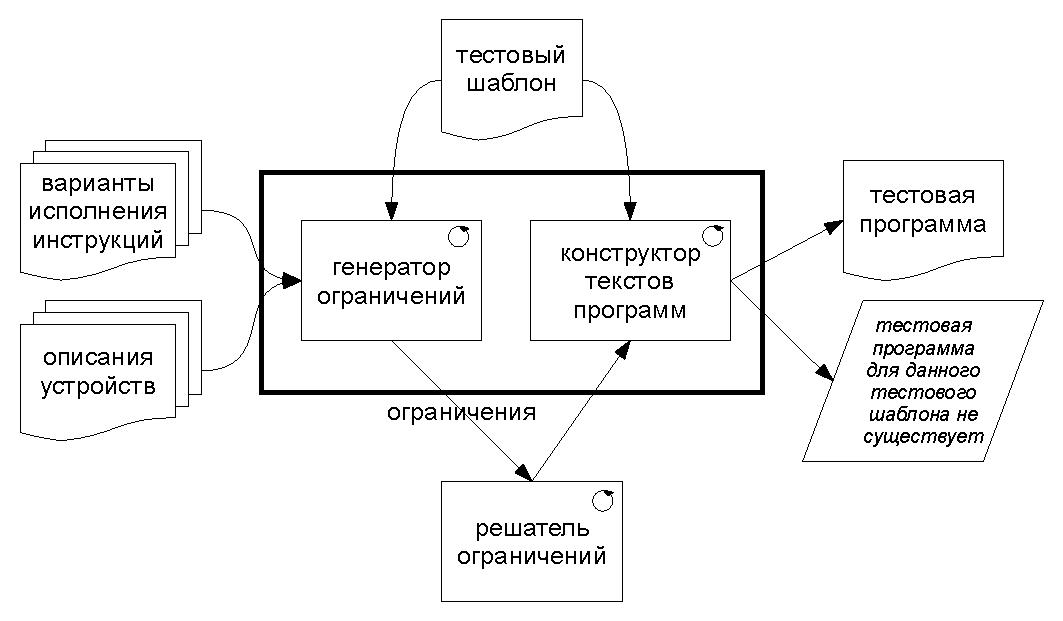
\includegraphics[width=0.8\textwidth]{2.theor/scheme}
  \caption{Программное средство для генерации тестовых программ}\label{fig:gen_scheme}
\end{figure}

Согласно схеме на рисунке~\ref{fig:gen_scheme} построение тестовой программы осуществляется следующим образом:
\begin{enumerate}
  \item \cmpn{Генератор ограничений} принимает на вход тестовый шаблон, описания вариантов исполнения инструкций и описания устройств подсистемы управления памяти и строит ограничения;
  \item Ограничения передаются на вход \cmpn{Решателю ограничений}; он определяет совместность данных ему ограничений; если ограничения несовместны, результатом его работы является сообщение о несовместности ограничений; если ограничения совместны, то он строит одно решение ограничений и сообщает это решение в качестве результата своей работы;
  \item \cmpn{Конструктор текстов программ} получает на вход тестовый шаблон и результат работы \cmpn{Решателя ограничений}; если \cmpn{Решатель ограничений} сообщил о несовместности ограничений, то \cmpn{Конструктор текстов программ} сообщает о несуществовании тестовой программы для данного тестового шаблона; иначе \cmpn{Конструктор текстов программ} на основе тестового шаблона по переданному \cmpn{Конструктору} решению ограничений строит тестовую программу, соответствующую тестовому шаблону.
\end{enumerate}

\begin{figure}[h] \center
  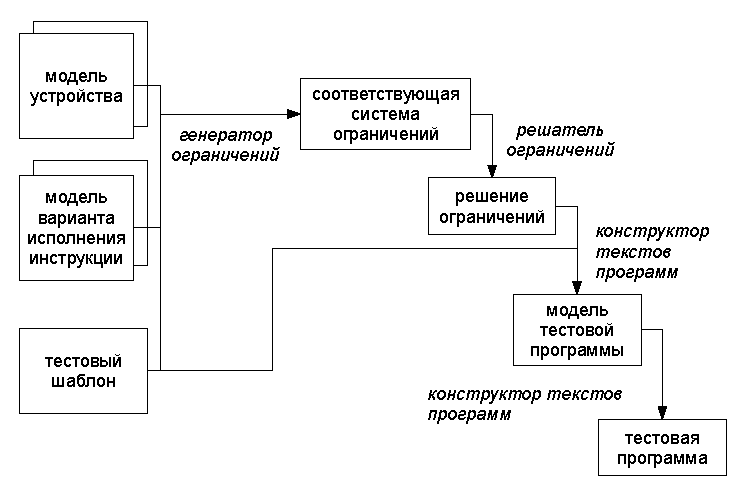
\includegraphics[width=0.8\textwidth]{2.theor/scheme2}
  \caption{Модели и задачи компонентов программного средства для генерации тестовых программ}\label{fig:models_tasks}
\end{figure}

Поставленная в разделе~\ref{sec:problem_refinement} задача решалась за счёт выбора специальных моделей (для вариантов исполнения инструкций, содержимого устройств подсистемы управления памяти и тестовой программы) и алгоритмов на основе этих моделей. На рисунке~\ref{fig:models_tasks} представлено место моделей в процессе генерации тестовой программы и задачи, которые решают компоненты описываемой здесь программной системы для генерации тестовых программ. В разделе~\ref{sec:state_model_section} будут даны формальные определения \emph{модели вариантов исполнения инструкций} и \emph{модели устройств}. В разделе~\ref{sec:constraints_generation_section} будет дано формальное определение \emph{системы ограничений, соответствующей} тестовому шаблону, моделям вариантов исполнения инструкций и моделям устройств. Неформально говоря, это такая система ограничений, которая эквивалентным образом выражает все ограничения на начальное состояние микропроцессора, содержащиеся в тестовом шаблоне и моделях. Задачей компонента \cmpn{Генератор ограничений} является построение системы ограничений, соответствующей тестовому шаблону, моделям вариантов исполнения инструкций и моделям устройств. Задачей \cmpn{Решателя ограничений} является разрешение этой системы ограничений. В разделе~\ref{?????} будет дано формальное определение \emph{модели тестовой программы} и \emph{модели тестовой программы, соответствующей решению ограничений и тестовому шаблону}. Неформально говоря, модель тестовой программы состоит из тестового шаблона, у каждой инструкции которого указаны значения ее аргументов, и последовательности адресов, по которым надо обратиться перед инструкциями тестового шаблона, и начальные значения регистров. Модель тестовой программы соответствует тестовому шаблону и решению ограничений, если в модели тестовой программы присутствует та же последовательность инструкций, а значения аргументов инструкций, адреса и начальные значения регистров взяты из решения ограничений. В разделе~\ref{????} будет дано формальное определение тестовой программы, соответствующей модели тестовой программы. Неформально говоря, это такая тестовая программа, которая исполняется в точном соответствии с моделью тестовой программы. Задачами компонента \cmpn{Конструктор тестовой программы} являются:
\begin{enumerate}
  \item построение модели тестовой программы, соответствующей тестовому шаблону и решению ограничений;
  \item построение тестовой программы, соответствующей модели тестовой программы.
\end{enumerate}




\section{Моделирование устройств подсистемы \\управления памяти и вариантов исполнения инструкций}\label{sec:state_model_section}

В данном разделе будут даны формальные определения ряда моделей%, будет уточнено определение тестового шаблона с учетом того, что эти шаблоны используются для тестирования подсистем управления памяти
. Будет дан ряд примеров и очерчена область применимости моделей.

\subsubsection*{Модель устройства подсистемы управления памяти}

%% определяется структура и содержание модельного состояния устройства

Назовем \emph{структурой поля} пару $(N, B)$, где $N$ --- произвольное имя, $B \in \mathds{N}$. $N$ будем называть \emph{именем} поля, $B$ --- \emph{битовой длиной} поля.

Назовем \emph{структурой строки} пару $(K, D)$, где $K$ и $D$ --- множества полей такие, что все поля в $K \cup D$ имеют разные имена. $K$ будем называть \emph{полями ключа}, $D$ будем называть \emph{полями данных}.

Назовем \emph{структурой региона} пару $(w, S)$, где $w \in \mathds{N}$, $S$ --- структура строки. $w$ будем называть \emph{ассоциативностью}.

Назовем \emph{структурной частью модели устройства} (или, \emph{структурой таблицы}) пару $(R, r)$, где $R \in \mathds{N} \cup \{0\}$, $r$ --- структура региона. Будем называть число $2^R$ \emph{количеством регионов}.

Назовем \emph{состоянием поля} со структурой $(N, B)$ целое число $v$ такое, что $v \geqslant 0$ и $v < 2^B$.

Назовем \emph{состоянием строки} со структурой $(K, D)$ пару $(k, d)$, где $K = \{K_1, K_2, ..., K_n\}$, $D = \{D_1, D_2, ..., D_m\}$, $k = \{k_1, k_2, ..., k_n\}$, $d = \{d_1, d_2, ..., d_m\}$, $k_i$ является состоянием поля $K_i$ для всех $i = 1, 2, ..., n$, $d_j$ является состоянием поля $D_j$ для всех $j = 1, 2, ..., m$.

Назовем \emph{состоянием региона} со структурой $(w, S)$ последовательность $\langle s_1,$ $s_2, ..., s_w\rangle$, где $r_i$ --- состояние строки со структурой $S$, $i = 1, 2, ..., w$, все состояния строк $s_j$ для $j = 1, 2, ..., w$ различные.

Назовем \emph{предикатом соответствия строки ключу} предикат $KM(k, \kappa)$, где $(k,d)$ --- состояние строки, $\kappa = (\kappa_1, \kappa_2, ..., \kappa_p)$, $\kappa_i \in \mathds{N} \cup \{0\}$, $i = 1, 2, ..., p$. Будем называть $\kappa$ \emph{ключом обращения}.

Назовем \emph{модельным состоянием устройства} со структурной частью $ST = (R, r)$ и предикатом соответствия строки ключу $KM$ последовательность $L = \langle r_0, r_1, ..., r_{2^R-1} \rangle$, где $r_i$ --- состояние региона со структурой $r$, $i = 0, 1, ..., 2^R{-}1$, и для любого состояния региона $r_i = \langle s_1, s_2, ..., s_w \rangle$ и для любого ключа обращения $\kappa$ не существует разных $s'$ и $s''$ из последовательности $r_i$ c состояниями полей ключей $k'$ и $k''$ соответственно таких, что $KM(k', \kappa)$ и $KM(k'', \kappa)$ истинны.


%% далее определяем правильные цепочки состояний
%%    с помощью определения правильных переходов между состояниями
%% > в результате будет определена `стратегия вытеснения'

Далее определим понятие <<стратегии вытеснения>> и ряда функций над модельными состояниями устройств.

Функция $hit: S \times \kappa \rightarrow S$, где $S$ --- состояние региона, $\kappa$ --- ключ обращения, определенная на тех парах $(S, \kappa)$, что в $S$ есть состояние строки $s = (k,d)$ такое, что $KM(k, \kappa)$ истинно, причем множество состояний строк в $hit(S, \kappa)$ и в $S$ одинаковые. Будем говорить, что в функции $hit$ осуществляется \emph{обращение к строке} $s$.

Функция $load: S \times \kappa \times dL \rightarrow S$, где $S$ --- состояние региона, $\kappa$ --- ключ обращения, $dL$ --- состояние полей данных, определенная на тех тройках $(S, \kappa, dL)$, что в $S$ есть состояние строки $s = (k,d)$ такое, что $KM(k, \kappa)$ истинно и $d = dL$, причем $load(S, \kappa, dL) = hit(S, \kappa)$. Будем говорить, что в функции $load$ осуществляется \emph{обращение к строке} $s$.

Функция $store: S \times \kappa \times dS \rightarrow S$, где $S$ --- состояние региона, $\kappa$ --- ключ обращения, $dS$ --- состояние полей данных, определенная на тех тройках $(S, \kappa, dS)$, что в $S$ есть состояние строки $s = (k,d)$ такое, что $KM(k, \kappa)$ истинно, причем выполнено следующее свойство: обозначим $store(S, \kappa, dS) = \langle r'_0, r'_1, ..., r'_{2^R-1}\rangle$ и $hit(S, \kappa) = \langle r''_0, r''_1, ..., r''_{2^R-1}\rangle$, $r''_i = s$, тогда $r'_j = r''_j$ для $j = 0, 1, ..., 2^R{-}1$, $j \neq i$, $r'_i = (k, dS)$. Будем говорить, что в функции $store$ осуществляется \emph{обращение к строке} $s$.

Функция $miss: S \times \kappa \rightarrow S$, где $S$ --- состояние региона, $\kappa$ --- ключ обращения, определенная на тех парах $(S, \kappa)$, что в $S$ нет состояния строки $s = (k,d)$ такого, что $KM(k, \kappa)$ истинно, и $miss(S, \kappa) = S$.

Назовем \emph{правилом определения вытесняемой строки} функцию $EV : S \rightarrow s$, где $S$ --- состояние региона, $s$ является состоянием одной из строк в $S$.

Функция $replace: S \times \kappa \times dR \rightarrow S$, где $S$ --- состояние региона, $\kappa$ --- ключ обращения, $dR$ --- состояние полей данных, определенная на тех тройках $(S, \kappa, dR)$, что в $S$ нет состояния строки $s = (k,d)$ такого, что $KM(k, \kappa)$ истинно, в состоянии региона $replace(S, \kappa, dR)$ есть состояние строки $s' = (\kappa, dR)$ и множество состояний строк в $S$ без состояния строки $EV(S)$ равно множеству состояний строк в $replace(S, \kappa, dR)$ без $s'$.

Назовем \emph{стратегией вытеснения} тройку функций $(hit, replace, EV)$.

Далее определим ряд семейств бинарных отношений над модельными состояниями устройств (другими словами, определим ряд \emph{параметризованных} бинарных отношений над модельными состояниями устройств, это означает, что каждому отношению будет сопоставлен ряд чисел и векторов чисел). Все определяемые далее бинарные отношения должны быть функциями, т.е. они должны определять однозначное соответствие (но не обязательно взаимно однозначное соответствие). По этой причине эти отношения будут далее в том числе использоваться как \emph{операции} над модельным состоянием.

Назовем \emph{отношением успешного обращения без данных} $Hit_{\kappa, \rho}$ множество пар модельных состояний $(L', L'')$, где $\kappa$ --- ключ обращения, $\rho$ --- целое число, $L' = \langle r'_0, r'_1, ..., r'_{2^R-1} \rangle$, $L'' = \langle r''_0, r''_1, ..., r''_{2^R-1} \rangle$, в которых выполнены все 3 следующие свойства:
  \begin{enumerate}
    \item $r''_i = r'_i$ для $i = 0, 1, 2, ..., 2^R{-}1$, $i \neq \rho$;
    \item в состоянии региона $r'_{\rho}$ существует строка $s = (k,d)$, для которой истинно $KM(k, \kappa)$;
    \item $r''_{\rho} = hit(r'_{\rho}, \kappa)$.
  \end{enumerate}

Назовем \emph{отношением успешного обращения с данными без изменения} (или, просто, \emph{отношением успешного обращения}) $HitLoad_{\kappa, \rho, dL}$ множество пар модельных состояний $(L', L'')$, где $\kappa$ --- ключ обращения, $\rho$ --- целое число, $dL$ --- состояние полей данных, $L' = \langle r'_0, r'_1, ..., r'_{2^R-1} \rangle$, $L'' = \langle r''_0, r''_1, ..., r''_{2^R-1} \rangle$, в которых выполнены все 3 следующие свойства:
  \begin{enumerate}
    \item $r''_i = r'_i$ для $i = 0, 1, 2, ..., 2^R{-}1$, $i \neq \rho$;
    \item в состоянии региона $r'_{\rho}$ существует строка $s = (k,d)$, для которой истинно $KM(k, \kappa)$ и $d = dL$;
    \item $r''_{\rho} = load(r'_{\rho}, \kappa, dL)$.
  \end{enumerate}

Назовем \emph{отношением успешного обращения без данных с изменением}\\ $HitStore_{\kappa, \rho, dS}$ множество пар модельных состояний $(L', L'')$, где $\kappa$ --- ключ обращения, $\rho$ --- целое число, $dS$ --- состояние полей данных, $L' = \langle r'_0, r'_1, ..., r'_{2^R-1} \rangle$, $L'' = \langle r''_0, r''_1, ..., r''_{2^R-1} \rangle$, в которых выполнены все 3 следующие свойства:
  \begin{enumerate}
    \item $r''_i = r'_i$ для $i = 0, 1, 2, ..., 2^R{-}1$, $i \neq \rho$;
    \item в состоянии региона $r'_{\rho}$ существует строка $s = (k,d)$, для которой истинно $KM(k, \kappa)$;
    \item $r''_{\rho} = store(r'_{\rho}, \kappa, dS)$.
  \end{enumerate}

Назовем \emph{отношением успешного обращения с данными с изменением} (или, просто, \emph{успешного обращения с изменением}) $HitLoadStore_{\kappa, \rho, dL, dS}$ множество пар модельных состояний $(L', L'')$, где $\kappa$ --- ключ обращения, $\rho$ --- целое число, $dL$ и $dS$ --- два состояния полей данных устройства, $L' = \langle r'_0, r'_1, ..., r'_{2^R-1} \rangle$, $L'' = \langle r''_0, r''_1, ..., r''_{2^R-1} \rangle$, в которых выполнены все 3 следующие свойства:
  \begin{enumerate}
    \item $r''_i = r'_i$ для $i = 0, 1, 2, ..., 2^R{-}1$, $i \neq \rho$;
    \item в состоянии региона $r'_{\rho}$ существует строка $s = (k,d)$, для которой истинно $KM(k, \kappa)$ и $d = dL$;
    \item $r''_{\rho} = store(r'_{\rho}, \kappa, dS)$.
  \end{enumerate}

Назовем \emph{отношением неуспешного обращения без замещения} $Miss(\kappa, \rho)$ множество пар модельных состояний $(L', L'')$, где $\kappa$ --- ключ обращения, $\rho$ --- целое число, $L' = \langle r'_0, r'_1, ..., r'_{2^R-1} \rangle$, $L'' = \langle r''_0, r''_1, ..., r''_{2^R-1} \rangle$, в которых выполнены все 3 следующие свойства:
  \begin{enumerate}
    \item $r''_i = r'_i$ для $i = 0, 1, 2, ..., 2^R{-}1$, $i \neq \rho$;
    \item в состоянии региона $r'_{\rho}$ нет состояния строки $s = (k,d)$, для которой истинно $KM(k, \kappa)$;
    \item $r''_{\rho} = miss(r'_{\rho}, \kappa)$.
  \end{enumerate}

Назовем \emph{отношением неуспешного обращения с замещением}\\ $MissReplace(\kappa, \rho, dR)$ множество пар модельных состояний $(L', L'')$, где $\kappa$ --- ключ обращения, $\rho$ --- целое число, $dR$ --- состояние полей данных, $L' = \langle r'_0, r'_1, ...,$ $r'_{2^R-1} \rangle$, $L'' = \langle r''_0, r''_1, ..., r''_{2^R-1} \rangle$, в которых выполнены все 3 следующие свойства:
  \begin{enumerate}
    \item $r''_i = r'_i$ для $i = 0, 1, 2, ..., 2^R{-}1$, $i \neq \rho$;
    \item в состоянии региона $r'_{\rho}$ нет строки $s = (k,d)$, для которой истинно $KM(k, \kappa)$;
    \item $r''_{\rho} = replace(r'_{\rho}, \kappa, dR)$.
  \end{enumerate}


Назовем \emph{моделью устройства} (или, \emph{таблицей}) тройку $(ST, RP, KM)$, где $ST$ --- структурная часть модели устройства, $RP$ --- стратегия вытеснения, $KM$ --- предикат соответствия строки ключу.

%% теперь вводим конечный автомат, раз он фигурирует в результатах автореферата!

Из введенной модели устройства следует представление устройства подсистемы управления памяти \emph{в виде конечного автомата}. Множеством состояний такого конечного автомата является множество всех модельных состояний (так, как они определены выше) и состояние Fail. Одно из модельных состояний выбрано в качестве начального состояния. Неформально говоря, к устройству производятся <<обращения>> с целью загрузить данные из устройства по заданному ключу в заданном регионе или сохранить данные в устройстве по заданному ключу в заданному регионе. Каждому обращению будет соответствовать один переход в конечном автомате. Переход помечен символом load, если это обращение с целью загрузки данных, или символом store, если это обращение с целью сохранения данных. Кроме того, символы load и store снабжены параметрами. load снабжен двумя параметрами: $\kappa$ (ключом обращения) и $\rho$ (номером региона). store снабжен тремя параметрами: $\kappa$ (ключом обращения), $\rho$ (номером региона) и $\delta$ (состоянием полей данных). Выходной алфавит конечного автомата состоит из символов $HitLoad$, $HitStore$ и $MissReplace$. Символ $HitLoad$ снабжен параметром $\delta$ (состояние полей данных). Функция переходов конечного автомата определено соответственно определениям отношений $HitLoad$, $HitStore$ и $MissReplace$, а именно:
  \begin{itemize}
    \item если для модельного состояния $L'$ существует такое модельное состояние $L''$, что $(L', L'') \in Hit_{\kappa, \rho}$, то из состояния $L'$ по входу load$(\kappa, \rho)$ осуществляется переход в состояние $L''$, при этом выходом является $HitLoad(\delta)$, где $\delta$ --- состояние полей данных такое, что $(L', L'') \in HitLoad_{\kappa, \rho, \delta}$; такой переход будет называться далее \emph{успешным обращением без изменения} (или, просто, \emph{успешного обращения});
    \item если для модельного состояния $L'$ не существует модельное состояние $L''$ такое, что $(L', L'') \in Hit_{\kappa, \rho}$, то из состояния $L'$ по входу load$(\kappa, \rho)$ осуществляется переход в состояние Fail;
    \item если для модельного состояния $L'$ существует такое модельное состояние $L''$, что $(L', L'') \in HitStore_{\kappa, \rho, \delta}$, то из состояния $L'$ по входу store$(\kappa, \rho, \delta)$ осуществляется переход в состояние $L''$, при этом выходом является\\ $HitStore$; такой переход будет называться далее \emph{успешным обращением c изменением};
    \item если для модельного состояния $L'$ существует такое модельное состояние $L''$, что $(L', L'') \in MissReplace_{\kappa, \rho, \delta}$, то из состояния $L'$ по входу store$(\kappa, \rho, \delta)$ осуществляется переход в состояние $L''$, при этом выходом является $MissReplace$; такой переход будет называться далее \emph{неуспешным обращением};
    \item все переходы из Fail ведут в Fail.
  \end{itemize}

Из определения отношений $HitStore$ и $MissReplace$ следует, что для любых $\kappa$, $\rho$, $\delta$ и для любого состояния $L'$, отличного от Fail, всегда есть либо переход из $L'$, помеченный $HitStore(\kappa, \rho, \delta)$, либо переход из $L'$, помеченный $MissReplace(\kappa, \rho, \delta)$.

Введенный таким образом конечный автомат позволяет по цепочке обращений в устройство из некоторого состояния определить, является ли эта цепочка обращений допустимой (т.е. приводит ли она в состояние Fail) и какие из обращений в этой цепочке были успешными, а какие были неуспешными.

% примеры моделей для устройств давать не буду, т.к. слишком много надо пояснять (почему LRU моделируется таким способом, почему регионы с вытеснением - это строки секций по одному и тому же индексу и т.д.)
% но можно ли тут сказать, что эту модель можно построить для практически полезных устройств? (кэш-память, TLB в MIPS, оперативная память)

% нотация
Для программной системы построения тестовых программ по тестовым шаблонам устройство подсистемы управления памяти должно быть представлено в рамках определенной в этом разделе модели устройства. Модель должна быть записана в виде \emph{описания устройства}. Описание устройства состоит из предиката соответствия строки ключу keyMatch и из пар <<название параметра = значение параметра>> для следующих параметров:
\begin{itemize}
    \item policy --- идентификатор, представляющий стратегию вытеснения (\LRU, \FIFO, \PseudoLRU); в число этих идентификаторов добавлен идентификатор none, он означает такую <<стратегию вытеснения>>, в которой нет функции replace и, соответственно, нет отношения $MissReplace$ (этот частный случай удобен при моделировании оперативной памяти, где отношения $Miss$ и $MissReplace$ по определению невозможны и при моделировании устройств, в которых неуспешные обращения не приводят к замещению);
    \item regionbits --- первый компонент структурной части модели устройства (двоичный логарифм количества регионов);
    \item lines --- количество строк в регионе (первый компонент структуры региона);
    \item line --- структура строки (для каждого поля указывается название, битовая длина, поле ли это ключа или поле данных).
%    \item keyMatch --- предикат от аргументов операции обращения и полей ключа строки; он истинен в том и только том случае, когда строка соответствует аргументам операции (тегам физического адреса, номерам виртуальных страниц и т.п.).
\end{itemize}

Пример описания кэш-памяти:
\begin{verbatim}
table L1 {
  policy = LRU;
  regionbits = 7;
  lines = 4;
  line( tag:24:key, d:32:data );
  keyMatch(kappa_tag:24) { kappa_tag = tag };
}
\end{verbatim}

Строка кэш-памяти состоит из поля tag, оно является полем ключа, и поля d. Ключ обращения состоит из одного компонента (kappa\_tag), его битовая длина равна 24 (т.е. kappa\_tag принимает целые значения от 0 до $2^{24}{-}1$. Ключ обращения соответствует строке, если kappa\_tag равен полю tag. Стратегия вытеснения LRU определяет такие правила перестановки строк, что в функции $replace$ замещается строка, последнее обращение к которой произошло раньше последнего обращения к любой другой строке региона. Детальное рассмотрение этой и других стратегий вытеснения будет сделано в разделе~\ref{sec:policy_table}.

%%% нужны пояснения ???

%Рассуждая для кэш-памяти (ее структура описана в разделе~\ref{section:cache}), строками будут кэш-строки с тегами адресов. Регион будут составлять кэш-строки из всех секций, расположенные по одному и тому же индексу. Количество строк в регионе  равно количеству секций, т.е. ассоциативности кэш-памяти $w$. Количество регионов равно количеству кэш-строк в секции.
%
%Буфер трансляции (TLB) в микропроцессорах архитектуры MIPS64~\cite{mips64III} состоит из строк, каждая строка содержит ряд полей, в том числе половину номера виртуальной страницы $v$, номер физического кадра, соответствующего виртуальной странице с номером $2v$, и номер физического кадра, соответствующего виртуальной странице с номером $2v+1$. Обращение в буфер происходит по некоторому виртуальному адресу. Если его половина присутствует в одной из строк TLB, то вычисляется физический адрес на основе одного из номеров физических кадров той же строки. Эту ситуацию будем считать <<попаданием>>. Если его половине не присутствует ни в одной из строк TLB, ситуацию будем считать <<промахом>>. При этом одна из строк будет вытеснена и заменена другой (это делается программно так же, как показано на рисунке~\ref{fig:blocks_init_examples}. Поэтому буфер трансляции адресов в микропроцессорах архитектуры
%MIPS64 моделируется таблицей из одного региона, каждая его строка состоит из полей \texttt{r}, \texttt{vpn/2}, \texttt{g}, \texttt{asid}, \texttt{pfn}$_0$, \texttt{CCA}$_0$, \texttt{v}$_0$, \texttt{pfn}$_1$, \texttt{CCA}$_1$, \texttt{valid}$_1$ и других.
%
%Упор на вытеснение сделан неслучайно: как показано в разделе~\ref{section:cache}, ряд важных ошибок связан именно с некорректной реализацией вытеснения. Предлагаемые здесь модели составляются для устройств подсистемы управления памяти, обладающих вытеснением. Это кэш-память всех уровней, таблицы трансляции адресов. Таким же образом можно смоделировать и оперативную память: строка такой таблицы содержит физический адрес и данные по нему, каждый регион состоит из одной строки.

%Описание модели уже упомянутого буфера трансляции адресов микропроцессоров архитектуры
%MIPS64 выглядит следующим образом:
%\begin{verbatim}
%table TLB
%{
%    line(   r:2:key, vpnd2:28:key, g:1:key, asid:4:key,
%            pfn0:24:data, cca0:3:data, valid0:1:data,
%            pfn1:24:data, cca1:3:data, valid1:1:data );
%    regionbits = 0;
%    policy = none;
%    lines = 48;
%    keyMatch(r:2, vpnd2:28) { .... };
%}
%\end{verbatim}
%
%Предикат keyMatch будет приведен чуть позже, когда будет описан для этого язык.




\subsubsection*{Модель варианта исполнения инструкций}

Напомню, что вариант исполнения инструкции --- это ограничение на значения аргументов инструкции и состояния микропроцессора, перед инструкцией и после нее.

%Здесь будет дано определение модели варианта исполнения инструкции.

%Представление варианта исполнения инструкции в рамках этой модели позволит увеличить при автоматизации построения тестовой программы для тестового шаблона

Назовем \emph{моделью варианта исполнения инструкции} для моделей устройств $M_1, M_2, ..., M_n$ пятерку $(Y, X, U, P, S)$, где
  \begin{itemize}
    \item $Y$ --- конечное множество переменных (множество \emph{выходных переменных});
    \item $X$ --- конечное множество переменных (множество \emph{входных переменных}), $X \cap Y = \varnothing$;
    \item $U$ --- конечное множество переменных (множество \emph{промежуточных переменных}), $U \cap Y = \varnothing$, $U \cap X = \varnothing$;
    \item $P$ --- ограничение над переменными $X \cup Y \cup U$;
    \item $S$ --- это множество троек $(M, r, p)$, где $M \in \{M_1, M_2, ..., M_n\}$, $r \in \{Hit,$ $HitLoad, HitStore, HitLoadStore, Miss, MissReplace\}$, $p$ --- это либо пара $(\kappa, \rho)$ при $r \in \{Hit, Miss\}$, либо тройка $(\kappa, \rho, d)$ при $r \in \{HitLoad,$ $HitStore, MissReplace\}$, либо четверка $(\kappa, \rho, dL, dS)$ при $r = HitLoadStore$, $\kappa$, $d$, $dL$, $dS$ --- последовательности переменных из множества $X \cup Y \cup U$, $\rho \in X \cup Y \cup U$, причем нет двух троек с одинаковым компонентом $M$.
  \end{itemize}

Тем самым модель указывает, что в рамках варианта исполнения инструкции допустим лишь определенный вид изменения модельного состояния устройств ($Hit$, $HitLoad$, $HitStore$, $HitLoadStore$, $Miss$ и $MissReplace$).

% нотация и семантика
Как и модели устройств, модели вариантов исполнения инструкций должны быть описаны на специальном языке для их использования в программной системе построения тестовых программ. Грамматика языка описания вариантов исполнения инструкции в виде расширенной формы Бэкуса-Наура приведена в приложении~\ref{sec:syntax}. Описание варианта исполнения инструкции состоит из двух частей: заголовка и тела описания. Заголовок состоит из объявлений аргументов инструкции. Объявление аргумента состоит из имени внутри данного описания и битовой длины аргумента. Аргументы в описаниях вариантов исполнения инструкций аналогичны формальным параметрам процедур в языке Паскаль с передачей аргументов по ссылке. Тело описания варианта исполнения инструкции состоит из последовательности \emph{операторов} над переменными-битовыми строками (let, assume) и операторов-обращений (hit, miss). Операторы над переменными-битовыми строками задают ограничение $P$, а операторы-обращения задают последовательность $\langle (r_i, p_i) \rangle_{i=1}^n$ (обозначения из определения модели варианта исполнения инструкции).

Семантика описаний вариантов исполнения инструкций представлена на языке RSL~\cite{RSL} в приложении~\ref{sec:semantics}. Назовем \emph{допустимым модельным состоянием} для модели варианта исполнения инструкции $(Y, X, U, P, S)$ вектор из значений всех переменных множества $X \cup Y \cup U$ и для каждой модели устройств подсистемы управления памяти бесконечная последовательность модельных состояний с указанием на одно из модельных состояний как на <<текущее>>. Каждому оператору в описании варианта исполнения инструкции сопоставим пару множеств допустимых модельных состояний $(PreS, PostS)$, причем $PostS \subseteq PreS$. Множество $PostS$ для произвольного (не последнего) оператора в описании варианта исполнения инструкции равно множеству $PreS$ для следующего оператора в этом же описании варианта исполнения инструкции. В приложении~\ref{sec:semantics} на языке RSL дано формальное определение допустимого модельного состояния и отношений над парами множеств допустимых модельных состояний $(PreS, PostS)$ для каждого оператора. Далее будут рассмотрены эти отношения для каждого оператора.

По определению множество допустимых модельных состояний $PostS$ последнего оператора в описании варианта исполнения инструкции включает лишь те модельные состояния устройств подсистемы управления памяти и значения переменных, из которых выполнены все операторы описания варианта исполнения инструкции. Если $PreS$ первого оператора в описании варианта исполнения инструкции включает все возможные допустимые модельные состояния, то $PostS$ последнего оператора этого описания варианта исполнения инструкции включает те и только те модельные состояния, на которых выполнены все операторы варианта исполнения инструкции. Описанию варианта исполнения инструкции соответствуют 2 множества допустимых модельных состояний: $PreS$ первого оператора в этом варианте исполнения инструкции и $PostS$ последнего оператора того же варианта исполнения инструкции. В тестовом шаблоне описания вариантов исполнения инструкций расположены в заданной последовательности, в которой $PostS$ для произвольного (не последнего) варианта исполнения инструкции совпадает с $PreS$ следующего за ним варианта исполнения инструкции. Тем самым, если $PreS$ первого описания варианта исполнения инструкции включает все возможные допустимые модельные состояния, то $PostS$ последнего описания варианта исполнения инструкции включает те и только те допустимые модельные состояния, на которых выполнены все варианты исполнения инструкции --- каждое такое допустимое модельное состояние задает \emph{начальное} состояний микропроцессора, из которого инструкции тестового шаблона будут исполняться согласно указанным вариантам исполнения. В это начальное состояние микропроцессора входят значения переменных, соответствующих регистрам микропроцессора, и первые элементы в последовательностях модельных состояний устройств.

$PostS$ \emph{оператора допущения} (\texttt{assume : boolexpr;}) равно множеству тех состояний из $PreS$, в которых для значений переменных выполнено логическое выражение \texttt{boolexpr}.

Входные и выходные переменные должны быть объявлены в заголовке описания варианта исполнения инструкции. А промежуточные переменные появляются внутри описаний вариантов исполнения инструкции --- для этого служит \emph{оператор объявления нового имени} let. Этот оператор имеет две формы: явную (\texttt{var <- expr;}) и неявную (\texttt{let var : BITLEN;}), \texttt{var} --- это имя переменной, \texttt{expr} --- выражение, \texttt{BITLEN} --- натуральное число. Оператор let в неявной форме объявляет промежуточную переменную \texttt{var} (т.е. в операторах описания варианта исполнения инструкции, расположенных до этого оператора let, переменной \texttt{var} нельзя пользоваться, после этого оператора --- можно) и фиксирует битовую длину ее значений, т.е. переменная может принимать любое целое значение от 0 до $2^{\mbox{\texttt{BITLEN}}}-1$. Иными словами, для оператора let в неявной форме $PostS$ равно $PreS$, причем все модельные состояния из $PostS$ отличаются лишь значением переменной \texttt{var} и среди всех модельных состояний из $PostS$ переменная \texttt{var} принимает все целые значения от 0 до $2^{\mbox{\texttt{BITLEN}}}-1$. Оператор let в явной форме является краткой записью такой последовательности операторов: \texttt{let var: BITLEN; assume: var = expr;}.

Операторам-обращения соответствуют следующие отношения над парами множеств модельных состояний $(PreS, PostS)$:
\begin{itemize}
  \item $PostS$ \emph{оператора попадания} \texttt{hit<table>(key, region) \{[loaded(} \\ \texttt{datafields)] [storing(datafields)]\}} равно множеству тех состояний из $PreS$, в которых текущее модельное состояния устройства table и следующее за ним модельное состояние устройства table находятся в отношении $p \in \{Hit, HitLoad, HitStore, HitLoadStore\}$, в этих отношениях состояние полей ключа $\kappa$ равно значению выражения \texttt{key} от значений переменных в допустимом модельном состоянии, а значение номера региона $\rho$ равно значению выражения \texttt{region} от значений переменных в допустимом модельном состоянии; синтаксис оператора попадания допускает наличие и отсутствие \texttt{loaded(datafields)} и \texttt{storing(datafields)}; если эти обе части отсутствуют, то $p = Hit$, если присутствует только \texttt{loaded}, то $p = HitLoad$, если присутствует только \texttt{storing}, то $p = HitStore$, в противном случае $p = HitLoadStore$, $datafields$ --- это последовательность выражений, задающая состояние полей данных;
  \item $PostS$ \emph{оператора промаха} \texttt{miss<table>(key, region) \{[replacing(} \\ \texttt{datafields)]\}} равно множеству тех состояний из $PreS$, в которых текущее модельное состояния устройства table и следующее за ним модельное состояние устройства table находятся в отношении $p \in \{Miss,$ $MissReplace\}$, в этих отношениях состояние полей ключа $\kappa$ равно значению выражения \texttt{key} от значений переменных в допустимом модельном состоянии, а значение номера региона $\rho$ равно значению выражения \texttt{region} от значений переменных в допустимом модельном состоянии; синтаксис оператора попадания допускает наличие и отсутствие \texttt{replacing(}\\ \texttt{datafields)}; в случае отсутствия \texttt{replacing} $p = Miss$, в противном случае $p = MissReplace$, $datafields$ --- это последовательность выражений, задающая состояние полей данных.
\end{itemize}

Неформально говоря, вариант исполнения инструкции описывается как последовательность уточнений состояния (assume), объявлений новых переменных (let) и обращений к устройствам подсистемы управления памяти (hit, miss).

Для составления выражений boolexpr и expr определены следующие <<операции>>~\cite{my_syrcose_2008, my_isp_2008}:
\begin{itemize}
    \item битовые операции:
        \begin{itemize}
            \item выделение бита с заданным индексом: \texttt{x[i]} есть значение \texttt{i}'го бита битовой строки \texttt{x};
            \item выделение диапазона бит в заданных границах: \texttt{x[i..j]} есть битовая строка, составленная из последовательности бит строки \texttt{x} с номерами \texttt{i}, \texttt{i+1}, ..., \texttt{j};
            \item битовая конкатенация: \texttt{x || y} есть битовая строка, первые биты которой равны битам строки \texttt{x}, а последующие --- битам строки \texttt{y};
            \item битовая степень: \texttt{x\^{ }n} есть битовая строка, равная $\underbrace{\mbox{\texttt{x||x||...||x}}}_{\mbox{\texttt{n}}}$;
            \item знаковое расширение битового размера: \texttt{(n) x} есть строка, битовая длина которой равна \texttt{n} и в знаковом представлении значение этой строки совпадает со значением строки \texttt{x};
        \end{itemize}
    \item арифметические операции (суммирование, вычитание, умножение); суммирование и вычитание производится только над числами одинаковой битовой длины по модулю, равному степени двойки с показателем, равным этой битовой длине; умножение есть в беззнаковой  (\texttt{*+}) и знаковой (\texttt{*-}) форме и проводится также над числами одинаковой битовой длины, но точно;
    \item отношения сравнения (равенство/неравенство, сравнение на\\больше~-~меньше);
    \item логические связки конъюнкция и дизъюнкция.
\end{itemize}

В приложении~\ref{sec:xml} приведен пример описания варианта исполнения инструкции загрузки данных из памяти целиком.

% границы применимости
Область действия моделей вариантов исполнения инструкций и языка описания вариантов исполнения инструкций позволяет выразить ряд структурных и функциональных особенностей организации устройств подсистемы управления памяти  и функциональных особенностей инструкций обращения в память, а именно:
\begin{itemize}
    \item многоуровневая кэш-память: для каждого уровня кэш-памяти составляется своя модель устройства, в вариантах исполнения инструкций явно указывается, в какие уровни происходят обращения, а в какие нет;
    \item обращение в память с использованием виртуальной памяти и без ее использования: эти два случая различаются классом виртуальных адресов (трансляция одного класса виртуальных адресов выполняется при помощи TLB, а другого класса --- без TLB), для указания класса виртуальных адресов достаточно добавить в ограничение $P$ модели варианта исполнения инструкции условие на виртуальный адрес;
    \item сквозная запись в память (write-through) и отложенная запись в память (write-back): в структуре строки модели устройства для кэш-памяти и в структуре строки модели устройства для оперативной памяти надо указать поля данных, а в описаниях вариантов исполнения инструкций явно указать изменение состояний этих полей при помощи storing в операторе hit;
    \item дополнительные условия на состояния полей ключа и данных: эти условия добавляются с помощью оператора assume;
    \item virtually indexed virtually tagged - кэш-память --- это кэш-память, в которой ключ и регион обращения вычисляются по виртуальному, а не физическому адресу (соответствующие выражения для состояний полей ключа и номеров регионов указываются в операторах-обращениях).
\end{itemize}

Ряд особенностей организации устройств подсистемы управления памяти не удается выразить в модели устройств и моделях вариантов исполнения инструкций~\cite{my_ewdts_2009}. Среди них:
\begin{itemize}
%    \item псевдослучайных действий: псевдослучайное вытеснение, псевдослучайный выбор таблицы, к которой происходит обращение;
    \item временн\'{ы}е ограничения: например, в некоторых микропроцессорах\\ PowerPC~\cite{PowerPC} трансляция адреса выполняется в два этапа: эффективный адрес (он содержит номер сегментного регистра и смещение в сегменте) сначала преобразуется в линейный (в нем нет номера сегментного регистра), затем линейный --- в физический; причем имеется буфер, который хранит пары из эффективного и физического адресов; во время трансляции одновременно выполняется обращение в этот буфер и двухэтапная схема; физический адрес считывается из того устройства, где быстрее будет получен физический адрес; тестовая ситуация, предписывающая выполнение трансляции в устройстве быстрее/медленнее, нежели чем через другое устройство, невыразима с использованием предлагаемого формализма;
    \item циклические действия с переменным числом итераций в описании инструкций: такие действия часто встречаются при задании алгоритмов работы FPU, однако на основе анализа документации по разным архитектурам был сделан вывод, что инструкции обращения к памяти с потоком управления, включающим такие итеративные действия, не сводящиеся к поиску строк и их вытеснению, как это определяется в операторах попадания и промаха, практически не встречаются;
    \item кэш-память инструкций, совместная кэш-память (с данными и инструкциями): кэш-память инструкций предназначена для кэширования блоков инструкций, тегами в строках кэш-памяти инструкций являются битовые части адресов, по которым расположены в памяти эти инструкции; однако в тестовых шаблонах инструкции расположены друг за другом, что не позволяет выразить многие тестовые ситуации на кэш-память инструкций; иными словами, для целенаправленной генерации тестовых программ на кэш-память инструкций нужная иная постановка задачи --- иначе тестовые ситуации, иные тестовые шаблоны, что выходит за рамки данной работы.
\end{itemize}


% модель программы

% соответствие модели программы и шаблона




%Теперь переходим к языку описания формализованных вариантов исполнения инструкций (или просто, языку описания инструкций). На предыдущих этапах вариант исполнения задавался в виде последовательности неформализованных действий. Формализованное описание инструкции повторяет эту последовательность, внося ряд уточнений. В документации по микропроцессору вариант исполнения инструкции описывается на псевдокоде в виде последовательности преобразований-операторов, причем большая их часть --- это операторы над битовыми строками (например, значениями регистров, виртуальных адресов, физических адресов). Предлагаемое в диссертации описание следует этому же принципу: это последовательность операторов над битовыми строками и двух дополнительных операторов, специфичных блокам подсистемы управления памяти.


%Далее будет рассмотрен ряд примеров описаний некоторых вариантов инструкций обращения к памяти.
%
%Рассмотрим на примере, как строится описание варианта инструкции LW под названием l1hit. В документации написано, что формат инструкции LW следующий:
%\begin{verbatim}
%LW rt, offset(base)
%\end{verbatim}
%
%Эта инструкция загружает в регистр rt 32 бита из памяти по (виртуальному) адресу base{+}offset. Описание функциональности инструкции LW в документации приводится на специальном псевдокоде (см. рисунок~\ref{fig:lw_exmp}).
%
%\begin{figure}[h]
%\begin{tabular}{cl}
%    ${ }^1$ & \texttt{vAddr <- sign\_extend(offset) + GPR[base]}\\
%    ${ }^2$ & \texttt{if vAddr[1..0] != 0\^{ }2 then}\\
%    ${ }^3$ & \hspace{2cm} \texttt{SignalException(AddressError)}\\
%    ${ }^4$ & \texttt{endif}\\
%    ${ }^5$ & \texttt{(pAddr, CCA) <- AddressTranslation(vAddr, DATA, LOAD)}\\
%    ${ }^6$ & \texttt{pAddr <- pAddr[PSIZE-1..3] || (pAddr[2..0] xor}\\
%       & \hspace{5cm} \texttt{(ReverseEndian || 0\^{ }2) )}\\
%    ${ }^7$ & \texttt{memdoubleword <- LoadMemory(CCA, WORD, pAddr, vAddr, DATA)}\\
%    ${ }^8$ & \texttt{byte <- vAddr[2..0] xor (BigEndianCPU || 0\^{ }2)}\\
%    ${ }^9$ & \texttt{GPR[rt] <- sign\_extend(memdoubleword[31+8*byte..8*byte])}\\
%\end{tabular}
%\caption{Описание инструкции LW на псевдокоде из документации по MIPS64}\label{fig:lw_exmp}
%\end{figure}
%
%Это описание представляет собой последовательность операторов, которые изменяют значения переменных и внутреннее состояние микропроцессора. В этом описании присутствует оператор присваивания (он обозначен обратной стрелкой <-) и условный оператор if-then-endif, в then-ветви которого находится оператор исключительной ситуации SignalException, прерывающий исполнение этой инструкции. GPR[rt] и GPR[base] --- это выражения для получения значений регистров общего назначения с именами rt и base соответственно. Также используется ряд других операций и констант (они набраны прописными буквами).
%
%В отдельной главе документации (2.2 Operation Section Notation and\\Functions) содержится описание <<подпрограмм>> AddressTranslation и\\LoadMemory. В первой происходит трансляция виртуального адреса в физический, во второй происходит обращение в оперативную память по физическому адресу с использованием кэш-памяти. В другой главе документации (4. Virtual Memory) указано, что в этих подпрограммах задействуются следующие устройства подсистемы управления памяти:
%\begin{itemize}
%  \item кэш-память данных первого уровня (D-cache);
%  \item кэш-память инструкций первого уровня (I-cache);
%  \item кэш-память второго уровня, совместная для данных и инструкций (L2-cache);
%  \item общий буфер трансляции адресов (TLB);
%  \item буфер трансляции адресов данных (DTLB);
%  \item буфер трансляции адресов инструкций (ITLB).
%\end{itemize}
%
%Вариант l1hit будет означать такое исполнение инструкции LW, при котором трансляция адреса выполняется без обращения к TLB и DTLB, а при обращении в кэш-память первого уровня происходит кэш-попадание.
%
%Тем самым для тестового шаблона будет задействована кэш-память данных первого уровня, значит, надо смоделировать устройство D-cache. Устройства I-cache и L2-cache и все *TLB не задействованы в l1hit, поэтому их моделировать не нужно.
%
%Составляем модель D-cache. Для этого читаем документацию и выделяем из нее:
%\begin{itemize}
%  \item ассоциативность равна 4;
%  \item стратегия вытеснения --- LRU;
%  \item размер виртуального адреса --- 64 бита;
%  \item размер физического адреса --- 36 бит; из них биты с 35го по 12й дают тег, с 11го по 5й --- дают номер региона, с 4го по 0й дают смещение в кэш-строке.
%\end{itemize}
%
%Тем самым, модель кэш-памяти первого уровня будет следующей:
%\begin{verbatim}
%    table l1 {
%        line(tag:24:key);
%        regionbits = 7;
%        policy = LRU;
%        lines = 4;
%        keyMatch(key:24) { key = tag };
%    }
%\end{verbatim}
%
%Кроме того, нужно будет получить значения из памяти (в memdoubleword). Значит, нужно смоделировать оперативную память:
%\begin{verbatim}
%    table memory {
%        line(phys:33:key; memdw:64:data);
%        regionbits = 0;
%        policy = none;
%        lines = 8589934592;
%    }
%\end{verbatim}
%
%Для подготовки формального описания l1Hit надо в описании инструкции LW:
%\begin{enumerate}
%  \item выделить аргументы инструкции и их битовые длины;
%  \item определить значения <<констант>> (в данном случае это PSIZE,\\ ReverseEndian, BigEndianCPU, WORD);
%  \item выделить в потоке управления этого описания путь, соответствующий варианту исполнения l1hit;
%  \item формализовать <<подпрограммы>> AddressTranslation и LoadMemory в контексте l1hit;
%  \item выразить выделенный путь в потоке управления в виде последовательности операторов.
%\end{enumerate}
%
%Аргументов здесь три: offset, GPR[base] и GPR[rt]. Их битовые длины -- 16, 64 и
%64 (первое написано также на странице описания LW, а остальные аргументы суть
%GPR --- регистры общего назначения, чей битовый размер в MIPS64 равен 64).
%<<Константы>> PSIZE, ReverseEndian, BigEndianCPU являются частью режима работы
%микропроцессора в момент тестирования. Тем самым их значения надо искать в этом
%режиме. Путь в потоке управления должен быть таким, чтобы в него попал
%LoadMemory (чтобы произошло заявленное кэш-попадание в кэш-память первого
%уровня).
%
%Начинаем строить формализованное описание варианта l1hit. Объявления аргументов:
%\begin{verbatim}
%    base : 64;
%    offset : 16;
%    rt : 64;
%\end{verbatim}
%
%Начало описания пути \texttt{l1Hit} практически дословно повторяет документацию (строки 1--4 описания инструкции LW):
%\begin{verbatim}
%    vAddr <- (64)offset + base;
%    assume: vAddr[1..0] = 0^2;
%\end{verbatim}
%
%В строке 5 идет <<вызов подпрограммы>> \texttt{AddressTranslation}. В l1hit трансляция виртуального адреса в физический должна выполняться без
%обращения к TLB. Это означает, что надо специфицировать условия, при которых
%трансляция адреса выполняется именно таким образом, и результат этой трансляции.
%Условия и результат трансляции описаны в документации (глава 4. Virtual memory). А именно, такая
%трансляция выполняется тогда, когда биты виртуального адреса с 58го по 36й равны нулю. В качестве результата формируется значение новых переменных --- физического адреса \texttt{pAddr} и политики кэширования \texttt{cca}:
%\begin{verbatim}
%    assume: vAddr[58..36] = 0^23;
%    pAddr <- vAddr[35..0];
%    cca <- vAddr[63..61];
%\end{verbatim}
%
%От политики кэширования будет зависеть работа кэш-памяти и это действительно
%разные способы работы -- сквозная запись и отложенная запись, где-то
%производится запись в кэш-память и в оперативную память, где-то только в
%оперативную память. Но при \texttt{l1Hit} запись не производится и
%поэтому достаточно, чтобы кэш-память просто была задействована. Согласно
%документации это означает, что \texttt{cca} не должно равняться 2. Тем самым
%появляется еще одно условие про \texttt{AddressTranslation}:
%\begin{verbatim}
%    assume: cca != 2;
%\end{verbatim}
%
%В строке 6 идет изменение физического адреса с учетом \texttt{ReverseEndian}.
%<<Константа>> ReverseEndian соответствует режиму, в котором происходит
%тестирование. Т.е. в момент генерации теста значение \texttt{ReverseEndian}
%известно, его не нужно искать с помощью ограничений. Если тест будет исполняться
%в режиме с \texttt{ReverseEndian = 0}, то преобразование выполнять не надо, т.к.
%\texttt{pAddr <- pАddr[PSIZE-1..3]||(pAddr[2..0] xor (0||0\^{ }2))} эквивалентно
%\texttt{pAddr <- pАddr[PSIZE-1..0])}, а \texttt{PSIZE = 36} (из документации),
%т.е. \texttt{pАddr[PSIZE-1..0]} получается то же, что и \texttt{pАddr}.
%Рассмотрим более сложный случай ---\\ \texttt{ReverseEndian = 1} (кроме того, хотя в документации используется одно и то же имя для физического адреса до изменения и после, при формализации надо указать новое имя):
%\begin{verbatim}
%    pAddr2 <- pAddr[35..3] || (pAddr[2]+1) || pAddr[1..0];
%\end{verbatim}
%
%В строке 7 идет <<вызов подпрограммы>> \texttt{LoadMemory}. В \texttt{l1Hit} это должно быть лишь
%обращение в кэш-память первого уровня с попаданием и обращение в память за
%данными. Надо понять, что является ключами и регионами этих обращений. Читаем
%документацию по тому, как проводится обращение в кэш-память:
%\begin{verbatim}
%    tag <- pAddr2[35..12];
%    region <- pAddr2[11..5];
%    phys <- pAddr2[35..3];
%    let data:64;
%    hit<l1>(tag, region){};
%    hit<memory>(phys){loaded(memdw=data)};
%\end{verbatim}
%
%Неявная форма оператора let была использована для получения значения поля memdw. Приведенная последовательность операторов фиксирует, что при обращение в \texttt{l1} должно быть успешным и
%из памяти считывается 64 бита в переменную \texttt{memdw}.
%
%В строках 8 и 9 из этих 64 бит выбираются 32 бита  --- старшая половина или младшая --- на основе значения \texttt{vAddr[2..0]}:
%\begin{verbatim}
%    byte <- vAddr[2..0];
%    let word:32;
%    assume: byte = 0 and word = memdw[31..0]
%         or byte = 4 and word = memdw[63..32];
%    rt <- (64)word;
%\end{verbatim}
%
%Описание инструкции \texttt{LW} для \texttt{l1Hit} готово. В правой половине рисунка~\ref{fig:l1hit_model} изображено формализованное описание варианта l1hit. В левой половине  рисунка~\ref{fig:l1hit_model} для сравнения приведен путь выполнения инструкции KW, которому соответствует l1hit.
%
%\begin{figure}[h]
%\noindent\parbox{0.4\textwidth}{ \footnotesize \tt
%vAddr <- sign\_extend(offset) + GPR[base];\\
%assume: vAddr[1..0] = 0\^{}2;\\
%(pAddr, CCA) <- AddressTranslation( vAddr, DATA, LOAD );\\
%pAddr <- pAddr[PSIZE-1..3] || (pAddr[2..0] xor (ReverseEndian || 0\^{}2 ));\\
%memdoubleword <- LoadMemory(CCA, WORD, pAddr, vAddr, DATA);\\
%byte <- vAddr[2..0] xor (BigEndianCPU || 0\^{}2);\\
%GPR[rt] <- sign\_extend( memdoubleword[ 31+8*byte .. 8*byte ] );\\
%} \parbox{0.1\textwidth}{ \quad
%} \parbox{0.5\textwidth}{ \footnotesize \tt
%base : 64;\\
%offset : 16;\\
%rt : 64;\\
%\\
%vAddr <- (64)offset + base;\\
%assume: vAddr[1..0] = 0\^{}2;\\
%assume: vAddr[58..36] = 0\^{}23;\\
%pAddr <- vAddr[35..0];\\
%cca <- vAddr[63..61];\\
%assume: cca != 2;\\
%pAddr2 <- pAddr[35..3] ||\\
%\indent\hspace{1cm}(pAddr[2]+1) || pAddr[1..0];\\
%tag <- pAddr2[35..12];\\
%region <- pAddr2[11..5];\\
%phys <- pAddr2[35..3];\\
%let data:64;\\
%hit<l1>(tag, region)\{\};\\
%hit<memory>(phys)\{loaded(memdw=data)\};\\
%byte <- vAddr[2..0];\\
%let word:32;\\
%assume: byte = 0 and word = data[31..0]\\
%\indent\hspace{1cm}or byte = 4 and word = data[63..32];\\
%rt <- (64) word;}
%\caption{Описание варианта l1hit до и после полной формализации}\label{fig:l1hit_model}
%\end{figure}
%
%Другим примером будет предикат keyMatch для TLB микропроцессоров MIPS64:
%(\texttt{asid} является <<константой>> режима тестирования, для примера
%допустим, что она равна 10)
%
%\begin{verbatim}
%table TLB
%{
%    line(   r:2:key, vpnd2:28:key, g:1:key; asid:4:key,
%            pfn0:24:data, cca0:3:data, valid0:1:data,
%            pfn1:24:data, cca1:3:data, valid1:1:data );
%    regionbits = 0;
%    policy = none;
%    lines = 48;
%    keyMatch(r1:2, vpnd:28) { r1 = r and vpnd = vpnd2 and
%        (g = 1 or asid = 10)};
%}
%\end{verbatim}


\section{Метод построения ограничений}\label{sec:constraints_generation_section}

В этом разделе будет формально поставлена задача, которую решает компонент \cmpn{Генератор ограничений} (см. схему на рисунке~\ref{fig:gen_scheme}), описано ее решение (алгоритм построения ограничений), обоснована корректность этого решения и исследован ряд свойств этого решения.

Задачей компонента \cmpn{Генератор ограничений} является построение системы ограничений, решение которой позволило бы построить тестовую программу для тестового шаблона. Для этого система ограничений должна <<соответствовать>> тестовому шаблону. В разделе~\ref{?????} дается формальное определение системы ограничений, соответствующей тестовому шаблону и моделям вариантов исполнения инструкций и устройств.

Неформально говоря, целью составления и разрешения системы ограничений является поиск значений операндов инструкций (как входящих в тестовый шаблон, так и дополнительных, \emph{инициализирующих} микропроцессор, которые помещаются в тестовую программу перед инструкциями из тестового шаблона), при которых возникнет заданная тестовым шаблоном тестовая ситуация (т.е. инструкции тестового шаблона будут выполнены согласно указанным для них вариантам исполнения).  Существует набор инструментов~\cite{Z3, Yices}, которые позволяют решить ограничения, поэтому ограничения должны принадлежать классам ограничений, с которыми умеют работать эти инструменты (известно, что с ограничениями в битовой арифметике и с ограничениями в линейной арифметике эти инструменты умеют работать).

Поскольку количество инструкций в тестовом шаблоне конечно, то в этих инструкциях осуществляются обращения лишь к конечному числу регионов устройств подсистемы управления памяти. Тем самым, необязательно при помощи ограничений искать всё целиком модельное состояние каждого устройства. Вместо этого достаточно искать состояния лишь необходимых для опе-раторов-обращений регионов модельных состояний (поскольку по определению отношений над парами модельных состояний одно обращение к устройству <<работает>> лишь с одним регионом, а состояния остальных регионов не изменяется). В некоторых случаях нет необходимости даже искать и состояние региона целиком (например, если в тестовом шаблоне есть всего один оператор-обращение к региону, причем это оператор попадания, тогда достаточно в инициализирующих инструкциях обеспечить 1 инструкцию, которая обратится в этот регион и обеспечит попадание). В разделе~\ref{?????} дается алгоритм построения системы ограничений. В нем учитываются высказанные в данном абзаце идеи по уменьшению количества переменных в ограничениях и количество самих ограничений, что, тем самым, позволяеь сократить вычислительную сложность разрешения ограничений.

Исполнение инструкций конвейеризовано, поэтому расположенные рядом инструкции в действительности будут выполняться параллельно в конвейере. Однако в алгоритме генерации ограничений считается, что инструкции выполняются последовательно, а тестовые шаблоны составлены таким образом, чтобы при работе соответствующих шаблонам тестовых программ проявились все выраженные в шаблонах параллельные эффекты.

В разделе~\ref{?????} формулируется и доказывается теорема корректности алгоритма построения ограничений. Эта теорема обосновывает тот факт, что предлагаемый в разделе~\ref{?????} алгоритм строит систему ограничений, соответствующую тестовому шаблону и моделям вариантов исполнения инструкций и устройств.

В разделе~\ref{?????} формулируется теорема полноты алгоритма построения ограничений. Эта теорема обосновывает тот факт, что множество значений переменных в тестовом шаблоне, соответствующих решению системы ограничений (построенной согласно этому алгоритму), а, соответственно, и множество тестовых программ для этих значений переменных в тестовом шаблоне, исчерпывает все возможные тестовые программы, удовлетворяющие тестовому шаблону. Иными словами, если построенная алгоритмам система ограничений окажется несовместной, то для тестового шаблона и моделей вариантов исполнения инструкций и устройств на самом деле не существует ни одной удовлетворяющей им тестовой программы.

%Формализовав устройства подсистемы управления памяти и инструкции и составив тестовый шаблон, нужно определить те значения регистров и хранящиеся данные устройств, при которых исполнение инструкций, указанных в тестовом шаблоне, будет проходить согласно указанным там вариантам. Для этого составляется система ограничений, выражающая все необходимые условия на такие значения. В результате разрешения этой системы определяются искомые значения. В данном разделе описывается предлагаемый алгоритм построения ограничений для тестового шаблона. Исполнение инструкций конвейеризовано, поэтому расположенные рядом инструкции в действительности будут выполняться с существенной долей параллелизма. Однако в алгоритме генерации ограничений считается, что инструкции выполняются последовательно, а тестовые шаблоны составлены таким образом, чтобы при работе соответствующих им тестовых программ проявились все нужные параллельные эффекты.
%
%По каждому оператору алгоритм строит свою часть ограничений, которые выражают семантику этого оператора. Операторы обращений в устройства транслируются в ограничения без моделирования состояний устройств, несмотря на то, что определение этих операторов включало состояние устройства. Это позволяет существенно уменьшить количество переменных-битовых строк и размер ограничений и, тем самым, ускорить разрешение ограничений. Специальное представление выбрано и для начального содержимого устройств, а именно, последовательность обращений в это устройство. Поэтому в число переменных в ограничениях входят переменные, задающие аргументы этих, \emph{инициализирующих}, обращений: ключи, номера регионов. Для операторов \texttt{hit} и \texttt{miss} строятся ограничения на аргументы-ключи и номера регионов (эти ограничения должны гарантировать успешное обращение для \texttt{hit} и неуспешное --- для \texttt{miss}) и ограничения на аргументы-данные из секций loaded, storing и replacing (обращения по одинаковым адресам должны давать одинаковые данные, если они не были изменены). Ограничения на аргументы-ключи и аргументы-номера регионов строятся согласно следующим определениям операторов: \texttt{hit(k$_i$;R$_i$)} / \texttt{miss(k$_i$;R$_i$)} происходит, если
%\begin{itemize}
%\item[$(\alpha)$] перед ним есть обращение по тому же ключу (\texttt{k}$_i$) в тот же регион (\texttt{R}$_i$),
%\item[$(\beta)$] после которого и до этого обращения соответствующая строка \underline{не была} \underline{вытеснена} / \underline{была вытеснена} из таблицы.
%\end{itemize}
%
%Трансляция свойства $\alpha$ достаточно очевидна, трансляция свойства $\beta$ рассматривается в разделе~\ref{sec:usefulness_functions}.

\subsection{Алгоритмы}

При формулировке алгоритмов будут использоваться следующие обозначения:
\begin{itemize}
  \item <<||>> --- битовая конкатенация;
  \item $[\varphi] \equiv $ if $\varphi$ then 1 else 0 endif.
\end{itemize}

\subsubsection*{Система ограничений, соответствующая тестовому шаблону, моделям устройств и вариантов исполнения инструкций}

Пусть задан следующий тестовый шаблон из $q$ инструкций для моделей устройств $M_1,$ $M_2,$ ..., $M_p$:

$I^{(1)}~a_1^{(1)}~a_2^{(1)}~...~a_{ac_1}^{(1)}~\mbox{@}~c^{(1)}( y_1^{(1)}, ..., y_{yc_1}^{(1)}, x_1^{(1)}, ..., x_{xc_1}^{(1)}, u_1^{(1)}, ..., u_{uc_1}^{(1)})$

$I^{(2)}~a_1^{(2)}~a_2^{(2)}~...~a_{ac_2}^{(2)}~\mbox{@}~c^{(2)}( y_1^{(2)}, ..., y_{yc_2}^{(2)}, x_1^{(2)}, ..., x_{xc_2}^{(2)}, u_1^{(2)}, ..., u_{uc_2}^{(2)})$

. . . . .

$I^{(q)}~a_1^{(q)}~a_2^{(q)}~...~a_{ac_q}^{(q)}~\mbox{@}~c^{(q)}( y_1^{(q)}, ..., y_{yc_q}^{(q)}, x_1^{(q)}, ..., x_{xc_q}^{(q)}, u_1^{(q)}, ..., u_{uc_q}^{(q)})$

где для каждого $i = 1, 2, ..., q$ $Y^{(i)} = \{ y_1^{(i)}, ..., y_{yc_i}^{(i)} \}$, $X^{(i)} = \{ x_1^{(i)}, ..., x_{xc_i}^{(i)} \}$, $U^{(i)} = \{ u_1^{(i)}, ..., u_{uc_i}^{(i)} \}$, $ac_i = yc_i + xc_i$, $Y^{(i)} \cap X^{(i)} = \varnothing$, $Y^{(i)} \cap U^{(i)} = \varnothing$, $X^{(i)} \cap U^{(i)} = \varnothing$, $c^{(i)} = (Y^{(i)}, X^{(i)}, U^{(i)}, P^{(i)}, Q^{(i)})$,

и для любых $i, j = 1, 2, ..., q$ таких, что $i \neq j$, $Y^{(i)} \cap Y^{(j)} = \varnothing$, $X^{(i)} \cap X^{(j)} = \varnothing$, $U^{(i)} \cap U^{(j)} = \varnothing$, $Y = \bigcup_{i=1}^q Y^{(i)}$, $X = \bigcup_{i=1}^q X^{(i)}$, $U = \bigcup_{i=1}^q U^{(i)}$, $Y \cap X = \varnothing$, $Y \cap U = \varnothing$, $X \cap U = \varnothing$,

для каждого $i = 1, 2, ..., q$ аргументам инструкции $I^{(i)}$ сопоставлены аргументы $c^{(i)}$: аргументу $a_1^{(i)}$ сопоставлено $y_1^{(i)}$, аргументу $a_2^{(i)}$ сопоставлено $y_2^{(i)}$, и т.д.

Тогда систему ограничений, удовлетворяющую всем следующим свойствам, будем называть \emph{соответствующей} тестовому шаблону, моделям вариантов инструкций и моделям устройств:
  \begin{enumerate}
    \item множество переменных системы ограничений равно множеству $Y \cup X \cup U \cup t \cup r \cup d$, где $t = \bigcup_{i=1}^p t^{(i)}$, $t^{(i)} = \{t_1^{(i)}, ..., t_{m_i}^{(i)}\}$, $r = \bigcup_{i=1}^p r^{(i)}$, $r^{(i)} = \{r_1^{(i)}, ..., r_{m_i}^{(i)}\}$, $d = \bigcup_{i=1}^p d^{(i)}$, $d^{(i)} = \{d_1^{(i)}, ..., d_{m_i}^{(i)}\}$, $t \cap r = \varnothing$, $t \cap d = \varnothing$, $r \cap d = \varnothing$, для всех допустимых различных $i'$ и $j'$ выполнено $t^{(i')} \cap t^{(j')} = \varnothing$, $r^{(i')} \cap r^{(j')} = \varnothing$, $d^{(i')} \cap d^{(j')} = \varnothing$, для всех $i'' = 1, 2, ..., q$ и различных $j'', j''' = 1, 2, ..., m_{i''}$ $t_{j''}^{(i'')} \neq t_{j'''}^{(i'')}$, $r_{j''}^{(i'')} \neq r_{j'''}^{(i'')}$, $d_{j''}^{(i'')} \neq d_{j'''}^{(i'')}$;

    \item для любого решения системы ограничений выполнены все следующие свойства:
        \begin{enumerate}
          \item для любых двух инструкций в тестовом шаблоне $I'$ и $I''$ (таких, что $I''$ идет после $I'$), среди аргументов которых встречается один и тот же аргумент $a$, который не встречается среди аргументов инструкций, расположенных в тестовом шаблоне между $I'$ и $I''$, если в $I'$ аргументу $a$ сопоставлен $x' \in X \cup Y$, а в $I''$ --- $x'' \in X$, то в решении системы ограничений переменные $x'$ и $x''$ имеют одинаковые значения;
          \item для каждого $i = 1, 2, ..., q$ предикат $P^{(i)}$ выполнен на значениях переменных из решения системы ограничений, соответствующих переменным из множеств $Y^{(i)}$, $X^{(i)}$ и $U^{(i)}$;
          \item для каждого $i = 1, 2, ..., p$ для любого модельного состояния $L_0^{(i)}$ устройства $M_i$ существует последовательность модельных состояний устройства $M_i$ $\langle L_{0;0}^{(i)}, L_{0;1}^{(i)}, L_{0;2}^{(i)}, ..., L_{0;m_i}^{(i)}, L_1^{(i)}, L_2^{(i)}, ..., L_q^{(i)}, L_{q+1}^{(i)} \rangle$ такая, что $L_{0;0}^{(i)} = L_0^{(i)}$, для каждого $j = 1, 2, ..., m_i$ $(L_{0;j-1}^{(i)}, L_{0;j}^{(i)}) \in HitStore^{(i)} (t_j^{(i)}, r_j^{(i)}, d_j^{(i)}) \cup MissReplace^{(i)} (t_j^{(i)}, r_j^{(i)}, d_j^{(i)})$, $L_{0;m_i}^{(i)} = L_1^{(i)}$ и для каждого $j = 1, 2, ..., q$ если в $Q^{(j)}$ есть тройка $(M_i, S_i, p_i)$, то $(L_j^{(i)}, L_{j+1}^{(i)}) \in S_i(p_i)$, где вместо переменных в $p_i$ подставлены значения соответствующих им переменных из решения ограничений, если же в $Q^{(j)}$ нет такой тройки, то $L_j^{(i)} = L_{j+1}^{(i)}$; $HitStore^{(i)}$ и $MissReplace^{(i)}$ соответствуют стратегии вытеснения в модели устройства $M_i$.
        \end{enumerate}
  \end{enumerate}

\paragraph{Основной алгоритм генерации ограничений} следующий:
\begin{enumerate}
    \item объединить последовательности операторов из описаний вариантов исполнения инструкций в порядке их упоминания в тестовом шаблоне в одну последовательность операторов;
    \item разделить полученную последовательность операторов на следующие подпоследовательности:
            \begin{itemize}
                \item первая подпоследовательность включает все операторы let и assume исходной последовательности (т.е. в этой подпоследовтельности находятся все предикаты $P$ из моделей вариантов исполнения инструкций);
                \item каждой другой подпоследовательности взаимно однозначно сопоставлено одно из устройств, в каждую такую подпоследовательность попадают все операторы-обращения к устройству, сопоставленному этой подпоследовательности (т.е. в этой подпоследовтельности находятся все тройки $(M, r, p)$ из моделей вариантов исполнения инструкций, в которых $M$ означает модель устройства, сопоставленного этой подпоследовательности);
            \end{itemize}
    \item транслировать операторы первой подпоследовательности в ограничения на битовые строки (из оператора <<assume: boolexpr>> таким ограничением становится boolexpr, из оператора <<var <- expr>> таким ограничением становится var = expr), иными словами, предикаты $P$ из моделей вариантов исполнения инструкций без изменения переходят в искомую систему ограничений (т.е. предикаты $P$ --- это предикаты над переменными-целыми числами ограниченной битовой длины, или, что то же самое, над битовыми строками);
    \item объявить переменные для аргументов описаний вариантов исполнения инструкций и состояний полей строк в операторах-обращениях для каждой подпоследовательности с шага 2 из операторов-обращений (т.е. искомая система ограничений формулируется над переменными, входящими в $X \cup Y \cup U$);
    \item для каждой построенной на шаге 2 подпоследовательности операторов-обращений выполнить
            \begin{enumerate}
                \item алгоритм генерации ограничений на ключи обращений;
                \item алгоритм генерации ограничений на загружаемые/сохраняемые данные.
            \end{enumerate}
\end{enumerate}

Введем следующее обозначение для задачи генерации ограничений на ключи обращений. Выберем устройство, обращения к которому будут составлять задачу, обозначим его модель $M$. Обозначим  последовательность $\{c^{(i)}\}_{i=1}^q$ моделей вариантов исполнения инструкций тестового шаблона, $c^{(i)} = (Y^{(i)}, X^{(i)},$ $U^{(i)},$ $P^{(i)}, Q^{(i)})$, $Q^{(i)}$ --- множество троек $(M', HM', HMA')$, где $M'$ --- модель одного из устройств, $HM' \in \{Hit, HitLoad, HitStore, HitLoadStore,$ $Miss,$ $MissReplace$ $\}$, в зависимости от значения $HM'$ $HMA'$ является парой, тройкой или четверкой, но в $HMA'$ обязательно присутствуют 2 переменные: первая $k'$ означает ключ обращения $k'$, вторая $R'$ --- номер региона. Из последовательности $\{c^{(i)}\}_{i=1}^q$ составим последовательность $\{Q^{(i)}\}_{i=1}^q$. Выберем из этой последовательности те элементы $Q^{(i)}$, где встречается тройка с моделью $M$. Далее в каждом элементе полученной последовательности оставим только ту тройку, в которую входит модель $M$. Получим последовательность $\{(M, HM'_j, HMA'_j)\}_{j=1}^n$. Составим по полученной последовательности следующую последовательность троек (назовем ее \emph{последовательность обращений к таблице}): $\{(S_j, k_j, R_j)\}_{j=1}^n$ (т.е. длина последовательности обращений к таблице будет обозначаться символом $n$), где $S_j$ = hit при $HM'_j \in \{Hit, HitLoad, HitStore, HitLoadStore\}$ и $S_j$ = miss при $HM'_j \in \{Miss, MissReplace\}$, а $k_j$ и $R_j$ --- переменные, означающие ключ обращения и номер региона из $HMA'_j$. Следующие алгоритмы генерации ограничений на ключи обращений предполагает, что на вход ему подана именно такая последовательность троек.

\subsubsection*{Алгоритм генерации ограничений на ключи обращений для таблицы, стратегия вытеснения которого есть \texttt{none}}

\begin{enumerate}
    \item выбрать подпоследовательность всех троек $(S, k, R)$ из данной последовательности обращений к таблице, в которых $S$ = hit; обозначить эту подпоследовательность $(S_1, k_1, R_1), ..., (S_N, k_N, R_N)$;
    \item для каждой тройки $(S, k, R)$ из данной последовательности обращений к таблице, в которой $S$ = miss, составить ограничение (если ключ обращения многомерный, то на месте символа $k$ в ограничениях должна стоять битовая конкатенация полей ключа обращения): $$(k||R) \notin \{(k_1||R_1), ..., (k_N||R_N)\}$$
    \item если $N > w$, где $w$ --- количество строк в регионе (т.е. значение параметра lines в описании устройства), то для каждого $l = w+1, w+2, \dots, N$ составить ограничение (<<в регионе не может быть больше различных строк, чем lines>>)
$$\sum_{i=1}^l [c_{R_l} (k_i, R_i)] \leqslant w$$
$$c_r (k_i, R_i) \equiv (R_i = r) \wedge \bigwedge_{j=1}^{i-1} (R_j \neq r \vee k_j \neq k_i)$$
\end{enumerate}

\subsubsection*{Алгоритм генерации ограничений на ключи обращений для таблицы,
стратегия вытеснения которой отлична от \texttt{none}}
поскольку алгоритм принимает на вход последовательность обращений к одной и той же таблице, то в обозначениях переменных по сравнению с определением системы ограничений, соответствующей моделям устройств и вариантов исполнения инструкций, будут отсутствовать надписи $(i)$, но будет подразумеваться, что везде речь идет про один и тот же $i = 1, 2, ..., p$, символом $m$ обозначено число $m_i$ из определения системы ограничений, соответствующей моделям устройств и вариантов исполнения инструкций: %~\cite{my_isp_2010}}:

\begin{enumerate}
    \item установить $m = n \cdot (n + 2\cdot w)$, где $n$ --- длина данной последовательности обращений к таблице, $w$ --- количество строк в регионе (т.е. значение параметра lines в описании устройства);
    \item в дополнение к уже объявленным переменным объявить переменные $t_1$, $t_2$, ..., $t_m$ (переменные для ключей обращений) и $r_1, r_2, ..., r_m$ (переменные для номеров регионов);
    \item составить ограничение <<все разные $(t_1||r_1), (t_2||r_2), ..., (t_m||r_m)$>>;
    \item для каждой тройки $(S_i, k_i, R_i)$ из данной последовательности обращений к таблице, в которой $S_i$ = hit, составить ограничения:
$$\left\{\begin{array}{l}
    (k_i||R_i) \in \{(t_1||r_1), (t_2||r_2), ..., (t_m||r_m), (k_1||R_1), ..., (k_{i-1}||R_{i-1}) \}\\
    \neg \mbox{displaced}(k_i, R_i)\\
\end{array}\right.$$

где предикат displaced$(k_i, R_i)$ истинен тогда и только тогда, когда с момента последнего вхождения $(k_i||R_i)$ в последовательность $\langle (t_1||r_1),$ $(t_2||r_2),$ ..., $(t_m||r_m), (k_1||R_1), ..., (k_{i-1}||R_{i-1})\rangle$ строка, на чьем поле ключа $k$ истинно $KM(k, k_i)$, вытеснена, т.е. после последнего вхождения $(k_i||R_i)$ есть оператор-обращение, в результате которого вытесняется строка, для полей ключа $k$ которой истинен $KM(k, k_i)$;

    \item для каждой тройки $(S_i, k_i, R_i)$ из данной последовательности обращений к таблице, в которой $S_i$ = miss, составить ограничения:
$$\left\{\begin{array}{l}
    (k_i||R_i) \in \{(t_1||r_1), (t_2||r_2), ..., (t_m||r_m), (k_1||R_1), ...,
(k_{i-1}||R_{i-1}) \}\\
    \mbox{displaced}(k_i, R_i)\\
\end{array}\right.$$

    \item если $n > w$, где $n$ --- длина данной последовательности обращений к таблице, $w$ --- количество строк в регионе (т.е. значение параметра lines в описании устройства), то для каждого $l = w+1, w+2, \dots, n$ составить ограничение (<<в регионе не может быть больше различных строк, чем lines>>)
$$\sum_{i=1}^l [c_{R_l} (k_i, R_i)] \leqslant w$$
$$c_{R_l} (k_i, R_i) \equiv (R_i = R_l ) \wedge \neg \mbox{displaced}_l (k_i, R_i) \wedge \bigwedge_{j=i+1}^{l} (R_j \neq R_l \vee k_j \neq k_i)$$
где предикат displaced$_l (k_i, R_i)$ истинен тогда и только тогда, когда среди операторов с $i+1$'го по $l$'й есть такой, в результате которого из региона с номером $R_i$ вытесняется строка, для полей ключа $k$ которой истинен предикат $KM(k, k_i)$.
\end{enumerate}

Предикаты displaced и displaced$_l$ отличаются лишь тем, начиная с какого оператора-обращения нужно проверять вытеснение. В случае displaced --- c первого инициализирующего обращения, в случае displaced$_l(k_i, R_i)$ --- с $i+1$'го. Поэтому далее речь будет идти про предикат displaced, но ровно то же самое переносится на предикат displaced$_l$.

Детальное исследование вопроса о том, как выразить предикат displaced (свойство <<быть вытесненным к моменту одного из обращений>>) в виде ограничений на битовые строки и линейную целочисленную арифметику дается в разделе~\ref{sec:usefulness_functions}.

\subsubsection*{Алгоритм генерации ограничений на поля данных в обращениях к таблицам}

Обозначим $M$ --- модель устройства, для обращений к которой применяется алгоритм.

\begin{enumerate}
  \item составить последовательность четверок $(A_j, k_j, R_j, d_j)$: обозначим  последовательность $\{c^{(i)}\}_{i=1}^q$ моделей вариантов исполнения инструкций тестового шаблона, $c^{(i)} = (Y^{(i)}, X^{(i)}, U^{(i)}, P^{(i)}, Q^{(i)})$, $Q^{(i)}$ --- множество троек $(M', HM', HMA')$, где $M'$ --- модель одного из устройств, $HM' \in \{Hit, HitLoad, HitStore, HitLoadStore, Miss, MissReplace\}$, в зависимости от значения $HM'$ $HMA'$ является парой, тройкой или четверкой, но в $HMA'$ обязательно присутствуют 2 переменные: первая $k'$ означает ключ обращения $k'$, вторая $R'$ --- номер региона; из последовательности $\{c^{(i)}\}_{i=1}^q$ составим последовательность $\{Q^{(i)}\}_{i=1}^q$; выберем из этой последовательности те элементы $Q^{(i)}$, где встречается тройка с моделью $M$; далее в каждом элементе полученной последовательности оставим только ту тройку, в которую входит модель $M$; получим последовательность $\{(M, HM'_j, HMA'_j)\}_{j=1}^{n'}$; уберем из этой последовательности тройки с $HM'_j \in \{Hit, Miss\}$; заменим в ней все тройки с $HitLoadStore$ $(M, HitLoadStore, (k', R', dL', dS'))$ на пару троек $(M, HitLoad, (k',$ $R',$ $dL')),$ $(M, HitStore, (k', R', dS'))$; получили последовательность троек\\ $\{(M, HM'_j, (k'_j, R'_j, d'_j))\}_{j=1}^n$; составим по полученной последовательности следующую последовательность четверок (назовем ее \emph{последовательность обращений с данными к таблице}) $\{(A_j, k_j, R_j, d_j)\}_{j=1}^n$ (т.е. длина последовательности обращений к таблице будет обозначаться символом $n$), где $A_j \in$ \{load, store\}, следующим образом: каждой тройке $(M, HM'_j, (k'_j, R'_j,$ $d'_j))$ сопоставим четверку $(A_j, k'_j, R'_j, d'_j)$, где $A_j$ = hit при $HM'_j = HitLoad$ и $A_j$ = miss при $HM'_j \in \{HitStore, MissReplace\}$, и поместим эти четверки в том же порядке, что и тройки $(M, HM'_j,$ $(k'_j,$ $R'_j, d'_j))$;
  \item для каждой четверки $(A_i, k_i, R_i, d_i)$, где $A_i$ = load, ввести переменные $v_{1;i}, v_{2;i}, ..., v_{i-1;i}, v_{i;i}$ и составить ограничения:
$$v_{i;i} = \mbox{~true}$$
$$v_{j;i} \equiv \begin{cases} \mbox{if~} (k_j||R_j = k_{j-1}||R_{j-1}) \mbox{~then~} d_j = d_{j-1} \mbox{~else~} v_{j-1;i} \mbox{~endif}, j{=}2,3,...,i\\
\mbox{true}, j{=}1\end{cases}$$
\end{enumerate}

\subsubsection*{Исследование описанных в этом разделе алгоритмов генерации ограничений}

Далее формулируется теорема~\ref{mirror_correctness} о том, что Основной алгоритм генерации ограничений строит систему ограничений, соответствующую тестовому шаблону, моделям вариантов исполнения инструкций и моделям устройств. Из очевидных соображений следует, что шаги Основного алгоритма и Алгоритма генерации ограничений на поля данных выполняют действия, сформулированные в определении системы ограничений, соответствующей тестовому шаблону, моделям вариантов исполнения инструкций и моделям устройств. Поэтому формулировка теоремы касается Алгоритма генерации ограничений на ключи обращений. В формулировку теоремы кроме последовательности обращений к таблице добавлено ограничение $P$ --- конъюнкция ограничений $P$ из моделей вариантов исполнения инструкций, входящих в тестовый шаблон.

\begin{theorem}[Корректность алгоритма генерации ограничений на ключи обращений]\label{mirror_correctness}
\CorrectnessMirror
\end{theorem}
\begin{proof}
  Предикат $P$ выполнен, потому что он, как есть, входит в систему ограничений (это следует из шага 3 Основного алгоритма генерации ограничений).

  Сначала рассмотрим таблицы, чья стратегия вытеснения не есть \texttt{none}. Для каждого $i = 1, 2, ..., n$ при $S_i${=}hit  $k_i$ и $R_i$ имеют такие значения, что для них выполнено свойство <<не быть вытесненным>>, это означает, что при обращении по этому ключу в этом регионе произойдет попадание. Аналогично для $S_i$ = miss.

  Теперь рассмотрим таблицы, чья стратегия вытеснения есть \texttt{none}. Разделим последовательность $\{(k_i, R_i)\}_{i=1}^n$ (часть решения системы ограничений) на подпоследовательности по значению $R_i$: все пары с одинаковым значением второго компонента будут образовывать одну подпоследовательность. Дальнейшее рассмотрение касается произвольной подпоследовательности (обозначим значение второго компонента пар в этой последовательности как $R$), оно без изменений переносится на все остальные подпоследовательности. Для любого ключа $k$, который входит в подпоследовательность обращений к таблице в тройке $($ miss, $k, R)$, из системы ограничений следует, что $(k||R) \notin \{(k_1||R_1), ..., (k_N||R_N)\}$. Поскольку для каждого $(k_i, R_i)$ $(k||R) = (k_i||R_i) \Leftrightarrow (k = k_i) \wedge (R = R_i)$, то ограничение на $(k||R)$ переписывается в виде $k \notin \{k_1, ..., k_{N'}\}$, где из множества удалены все ключи обращений $k_i$, для которых $R_i \neq R$. Обозначим $L_0 = \{k_1, ..., k_{N'}\}$. Если $|L_0| = w$, то положим $L'_0 = L_0$, иначе положим $L'_0 = L_0 \cup \{l_1, ..., l_{N''}\}$, где $l_1, ...., l_{N''}$ --- различные ключи такие, что $L_0 \cap \{l_1, ..., l_{N''}\} = \varnothing$ и $|L'_0| = w$. Таким образом, будет построено множество $L'_0$, состоящее из $w$ различных ключей обращений, причем любой ключ $k$, который входит в последовательность обращений к таблице в тройке $($ hit, $k, R)$, принадлежит этому множеству, а любой ключ $k$, который входит в последовательность обращений к таблице в тройке $($ miss, $k, R)$, не принадлежит этому множеству. Тем самым показано, что решение системы ограничений удовлетворяет последовательности $S_1, S_2, ..., S_n$.
\end{proof}

% доказательство для случая none кривое? надо еще показать, связь с t_i, а то получается, что теорема доказана не для любого начального состояния региона, а для некоторого специального

Иными словами, множество переменных в системе ограничений, которую строят описанные в этом разделе алгоритмы, совпадает с тем множеством, которое требуется в определении <<соответствующей системы ограничений>>, ограничения $P^{(i)}$ из моделей вариантов исполнения инструкций переходят в систему ограничений без изменений, для ключей обращения система ограничений, которую строят описанные в этом разделе алгоритмы, имеет множество решений, удовлетворяющих указанным в тестовом шаблоне отношениям $Hit...$ и $Miss...$. Ограничения, генерируемые алгоритмом на поля данных, в точности выражают свойство, что для любых двух обращений к таблице (из которых второе --- load) выполнено свойство: если в этих обращениях задействован один и тот же регион и одна и та же строка региона, то в этих строках должны совпадать состояния полей данных, если между этими обращениями нет других обращений к той же строке (повторное обращение по тому же <<адресу>> должно давать те же данные, если данные между обращениями не менялись). Тем самым, представленные в данном разделе алгоритмы строят систему ограничений, соответствующую тестовому шаблону, моделям вариантов исполнения инструкций и моделям устройств.

Следующие две теоремы формулируют свойство <<полноты>> системы ограничений, которую строят представленные в данном разделе алгоритмы. Неформально говоря, <<полнота>> означает, что алгоритмы строят такую систему ограничений, чье множество решений исчерпывает все возможные значения переменных, входящих в тестовый шаблон, при которых выполнены все ограничения в тестовом шаблоне.

\begin{theorem}[Полнота алгоритма генерации ограничений на ключи обращений для таблицы, стратегия вытеснения которой есть \texttt{none}]\label{mirror_fullness_none}
\FullnessMirrorNone
\end{theorem}

\begin{theorem}[Полнота алгоритма генерации ограничений на ключи обращений для таблицы, стратегия вытеснения которой не \texttt{none} и является \textbf{существенно вытесняющей}]\label{mirror_fullness}
\FullnessMirror
\end{theorem}

В приложении~\ref{sec:proofs} приведены доказательства теорем~\ref{mirror_fullness_none} и \ref{mirror_fullness}. Понятие <<существенно вытесняющей>> стратегии вытеснения дается в разделе~\ref{sec:essentially_displacing}. Неформально говоря, это такая стратегия вытеснения, в которой последовательные промахи в один регион приводят к полному перезаполнению состояния региона таблицы. В разделе~\ref{sec:essentially_displacing} доказывается, что к таким стратегиям вытеснения относятся \LRU, \FIFO и \PseudoLRU~---~это те стратегии вытеснения, которые используются в большинстве микропроцессоров, что демонстрирует практическую применимость теорем о полноте.

Длина инициализирующей последовательности обращений (эта последовательность обозначалась $t_1, t_2, ..., t_m$ (ключи обращений) и $r_1, r_2, ..., r_m$ (номера регионов)) $m$ должна быть достаточной, чтобы в результате исполнения инициализирующей последовательности обращений обеспечить специальное модельное состояние устройства перед первой инструкций тестового шаблона --- чтобы к моменту первой инструкции тестового шаблона в модельном состоянии заведома были определенные строки и заведома не было ряда других строк. Из доказательства теоремы~\ref{mirror_fullness} следует, что $m \leqslant r \cdot (\max(n,w) + w) \leqslant r \cdot (n + w + w)$, где $r \equiv |\{R_1, R_2, ..., R_n\}|$. Очевидно, что $r \leqslant n$, поэтому $m \leqslant n \cdot (n + 2\cdot w)$.

Можно рассматривать класс алгоритмов генерации ограничений на ключи обращений, различающихся значением $m$ (от 0 до $n(n+2w)$). Меньшее значение $m$ (т.е. более короткая инициализирующая последовательность обращений) дает и более короткую тестовую программу. Более короткие тестовые программы обладают лучшими техническими характеристиками (такими как время исполнения, размер программы в памяти), особенно важными при использовании тестовых программ на практике, где количество тестовых программ измеряется десятками и сотнями тысяч. Возможна и модификация алгоритма генерации ограничений на ключи обращений, в котором вся цепочка построения тестовой программы проводится несколько раз, каждый раз с разным значением $m$, не превышающим $n(n+2w)$. Такой алгоритм позволяет подобрать минимальное значение $m$, при котором генерируемая система ограничений совместна.

Следующая теорема показывает, что для стратегии вытеснения \LRU достаточно использовать значения $m$, меньшие $n(n+2w)$:

\begin{theorem}[Верхняя оценка достаточного количества инициализирующих обращений для
стратегии вытеснения \LRU]\label{thm_mirror_lenth_lru} \UpperBoundLRUMirror
\end{theorem}
Доказательство теоремы приведено в приложении~\ref{sec:proofs}.
%\begin{sld} Для \LRU
%      $$m = O(n)$$
%\end{sld}


%Следующий вопрос, как выбирать длину инициализирующей программы $m$. % Из леммы .......... следует, что такая длина существует для любой последовательности обращений в таблицу.
%Доказательство теоремы о полноте дает верхнюю оценку: $m = O(n^2)$ (см. раздел~\ref{sec:essentially_displacing}). Однако в конкретных случаях возможны более сильные верхние оценки для $m$. Так в разделе~\ref{sec:essentially_displacing} приведена верхняя оценка $m$ для стратегии вытеснения \LRU, линейно зависимая от длины последовательности обращений (ее доказательство --- в приложении~\ref{sec:proofs}). Этот факт делает эффективным использование алгоритмов типа дихотомии для поиска минимального значения $m$ для данной последовательности обращений (минимизация ведет к уменьшению размеров будущих тестовых программ и, как следствие, ускорению тестирования).

\subsection{Таблицы вытеснения (policy table)}\label{sec:policy_table}

Таблицы вытеснения были предложены в 2008 году исследователями из немецкого университета Саарланда~\cite{policy_tables}. Таблица вытеснения однозначно описывает изменение порядка и вытеснение строк региона. Тем самым таблица вытеснения есть метод формального описания стратегии вытеснения.

Таблица вытеснения исходит из \emph{перестановочной интерпретации} стратегии
вытеснения. Она состоит в том, что строки в регионе упорядочены, каждое
обращение к таблице осуществляет перестановку строк региона.
Никакие дополнительные данные (счетчики, строки, деревья) при этом не используются. Можно понимать эти перестановки и как перестановки <<позиций строк>>.
Определение вытесняемого элемента тоже осуществляется лишь на основе текущих
позиций строк. Таблица вытеснения как раз фиксирует выполняемые перестановки.

Таблица вытеснения представляет собой матрицу $(w{+}1) \times (w{+}1)$, где $w$
--- ассоциативность таблицы (количество строк региона). Первый столбец ---
специальный, он содержит указание позиций от 0 до $w{-}1$ (для успешных обращений) и специальную <<псевдопозицию>> для неуспешных обращений (символ $\pi$ помогает
указанию того, что речь идет о позициях). Остальными элементами
матрицы являются числа от 0 до $w{-}1$ и специальный символ $m$ для
вытесняющего ключа. Пример таблицы вытеснения (для стратегии
вытеснения \LRU) приведен на рисунке~\ref{fig:PolicyTableLRU8}.

\begin{figure}[h]
$$ \left[
     \begin{array}{c|cccccccc}
       \pi_0 & 0 & 1 & 2 & 3 & 4 & 5 & 6 & 7 \\
       \pi_1 & 1 & 0 & 2 & 3 & 4 & 5 & 6 & 7 \\
       \pi_2 & 2 & 0 & 1 & 3 & 4 & 5 & 6 & 7 \\
       \pi_3 & 3 & 0 & 1 & 2 & 4 & 5 & 6 & 7 \\
       \pi_4 & 4 & 0 & 1 & 2 & 3 & 5 & 6 & 7 \\
       \pi_5 & 5 & 0 & 1 & 2 & 3 & 4 & 6 & 7 \\
       \pi_6 & 6 & 0 & 1 & 2 & 3 & 4 & 5 & 7 \\
       \pi_7 & 7 & 0 & 1 & 2 & 3 & 4 & 5 & 6 \\
       \pi_m & m & 0 & 1 & 2 & 3 & 4 & 5 & 6 \\
     \end{array}
   \right]
$$
\caption{Таблица вытеснения для стратегии вытеснения \LRU,
8-ассоциативная таблица}\label{fig:PolicyTableLRU8}
\end{figure}

Строки таблицы вытеснения, кроме последней, описывают перестановку позиций строк
региона при обращении с попаданием. Каждой такой строке соответствует попадание
на позицию, которая указана в первом столбце строки. Остальная часть строки есть
перестановка позиций строк (0~1~...~$w{-}1$). Например, для стратегии вытеснения
\LRU,
представленной на рисунке~\ref{fig:PolicyTableLRU8}, при попадании по позиции 5
строки таблицы, пронумерованные как (4 6 5 7 1 0 2 3), будут переставлены
(смотрим строку с $\pi_2$, потому что позиция 5 находится на позиции c номером
2) согласно (2 0 1 3 4 5 6 7), что даст в результате новое расположение этих
строк как (5 4 6 7 1 0 2 3).

Последняя строка таблицы вытеснения соответствует обращению с промахом.
Вытесняющая строка помечается буквой $m$. Позиция вытесняемой строки --- тот
элемент набора (0~1~... $w{-}1$), который отсутствует в последней строке таблицы
вытеснения. Например, в таблице вытеснения на рисунке~\ref{fig:PolicyTableLRU8}
позиция вытесняемой строки равна 7, т.е. вытесняется последняя строка, а
вытесняющая помещается в самое начало со сдвигом оставшихся строк.

В качестве другого примера приведем таблицы вытеснений для других двух стратегий
вытеснения -- \FIFO и \MRU (см. рис.~\ref{fig:fifo_mru_tables}).

\begin{figure}[h] \centering
\parbox{0.4\textwidth}{
$$ \left[
     \begin{array}{c|cccccccc}
       \pi_0 & 0 & 1 & 2 & 3 & 4 & 5 & 6 & 7 \\
       \pi_1 & 0 & 1 & 2 & 3 & 4 & 5 & 6 & 7 \\
       \pi_2 & 0 & 1 & 2 & 3 & 4 & 5 & 6 & 7 \\
       \pi_3 & 0 & 1 & 2 & 3 & 4 & 5 & 6 & 7 \\
       \pi_4 & 0 & 1 & 2 & 3 & 4 & 5 & 6 & 7 \\
       \pi_5 & 0 & 1 & 2 & 3 & 4 & 5 & 6 & 7 \\
       \pi_6 & 0 & 1 & 2 & 3 & 4 & 5 & 6 & 7 \\
       \pi_7 & 0 & 1 & 2 & 3 & 4 & 5 & 6 & 7 \\
       \pi_m & m & 0 & 1 & 2 & 3 & 4 & 5 & 6 \\
     \end{array}
   \right]$$
\center \FIFO} \qquad
\parbox{0.4\textwidth}{
$$ \left[
     \begin{array}{c|cccccccc}
       \pi_0 & 1 & 2 & 3 & 4 & 5 & 6 & 7 & 0 \\
       \pi_1 & 0 & 2 & 3 & 4 & 5 & 6 & 7 & 1 \\
       \pi_2 & 0 & 1 & 3 & 4 & 5 & 6 & 7 & 2 \\
       \pi_3 & 0 & 1 & 2 & 4 & 5 & 6 & 7 & 3 \\
       \pi_4 & 0 & 1 & 2 & 3 & 5 & 6 & 7 & 4 \\
       \pi_5 & 0 & 1 & 2 & 3 & 4 & 6 & 7 & 5 \\
       \pi_6 & 0 & 1 & 2 & 3 & 4 & 5 & 7 & 6 \\
       \pi_7 & 0 & 1 & 2 & 3 & 4 & 5 & 6 & 7 \\
       \pi_m & 0 & 1 & 2 & 3 & 4 & 5 & 6 & m \\
     \end{array}
   \right]$$
\center \MRU } \caption{Таблицы вытеснения для 8-ассоциативной
таблицы}\label{fig:fifo_mru_tables}
\end{figure}

\subsection{Существенно вытесняющие стратегии вытеснения}\label{sec:essentially_displacing}

Стратегию вытеснения будем называть \emph{существенно вытесняющей}, если $w$ промахов в один регион полностью вытесняют его предыдущее содержимое.

С использованием аппарата таблиц вытеснения дадим другое определение существенно вытесняющей стратегии вытеснения. Обозначим $T_m$ --- последнюю строку таблицы вытеснения (перестановку, соответствующую промаху). Тогда стратегия вытеснения называется существенно вытесняющей, если $$(0~1~2~\dots~w{-}1) \cdot T_m^w = (\underbrace{m~m~\dots~m}_{\mbox{$w$~раз}})$$ где $w$ --- размерность перестановки (ассоциативность таблицы).

\begin{theorem}\label{thm:LRU_essential}
  Стратегия вытеснения \LRU является существенно вытесняющей.
\end{theorem}
\begin{proof}
  Для \LRU последняя строка таблицы вытеснения имеет вид: $T_m = (m~0~1~2~\dots~w{-}2)$ Поэтому
  $$(0~1~2~\dots~w{-}1) \cdot T_m = (m~0~1~2~\dots~w{-}2)$$
  $$(0~1~2~\dots~w{-}1) \cdot T_m^2 = (m~m~0~1~\dots~w{-}3)$$
  $$\mbox{...}$$
  $$(0~1~2~\dots~w{-}1) \cdot T_m^w = (m~m~m~\dots~m)$$
\end{proof}

\begin{theorem}
  Стратегия вытеснения \FIFO является существенно вытесняющей.
\end{theorem}
\begin{proof}
  Для \FIFO последняя строка таблицы вытеснения совпадает с таковой для \LRU. Поэтому доказательство этой теоремы идентично доказательству теоремы~\ref{thm:LRU_essential}.
\end{proof}

\begin{theorem}\label{thm:PseudoLRU_essential} \PseudoLRUEssential \end{theorem}

Доказательство этой теоремы находится в приложении~\ref{sec:proofs}.



\section{Новое определение стратегии вытеснения\\ \PseudoLRU}\label{sec:plru_new_definition}

Стратегия вытеснения \LRU хоть и хорошо приближает поведение
таблицы к идеальному случаю (когда данные находятся в
таблице в тот момент, когда они нужны), однако все известные на
сегодняшний момент реализации \LRU для микропроцессоров требуют большого
количества дополнительной логики. Поэтому производятся поиски
стратегии вытеснения, близкой по эффективности к \LRU, но имеющей
реализацию с меньшими накладными расходами. Эти поиски привели к
стратегии вытеснения \PseudoLRU. Она используется в микропроцессорах архитектур
PowerPC~\cite{PowerPC} и IA-32~\cite{FundamentalOfComputerOrganizationAndDesign}.

\subsubsection{Каноническое определение \PseudoLRU на бинарном дереве}

Следующее описание часто встречается в
литературе~\cite{FundamentalOfComputerOrganizationAndDesign} при
определении \PseudoLRU. Оно формулируется на
упорядоченном бинарном дереве высоты $\log_2 w$, в листьях которого
подряд расположены строки (их количество равно $w$). Стратегия вытеснения
\PseudoLRU определяется только для таблиц с ассоциативностью, являющейся степенью двойки, поэтому число $\log_2 w$ является натуральным. Каждая душа дерева помечена цифрой 0 (<<дуга идет налево>>) или цифрой 1 (<<дуга идет направо>>). Вершины тоже помечаются цифрами 0 или 1. Стратегия вытеснения определяется как процесс изменения пометок в вершинах дерева.

Успешному обращению в таблицу всегда соответствует некоторая (единственная) строка, значит, и некоторая листовая вершина дерева. При неуспешном обращении определена (единственная) вытесняемая строка, а, значит, определена и соответствующая этой строке листовая вершина дерева. В результате обращения меняются пометки в нелистовых вершинах пути от корня до этой листовой вершины (см. рис.~\ref{pseudo_lru_hit}). А именно вершина получает пометку
исходящей из нее дуги согласно этому пути. Т.е. если дуга, соответствующая пути, выходит влево, вершина помечается цифрой 0, если вправо -- 1 (старая пометка вершины забывается). Пометки остальных вершин дерева не меняются.

\begin{figure}[h] \center
  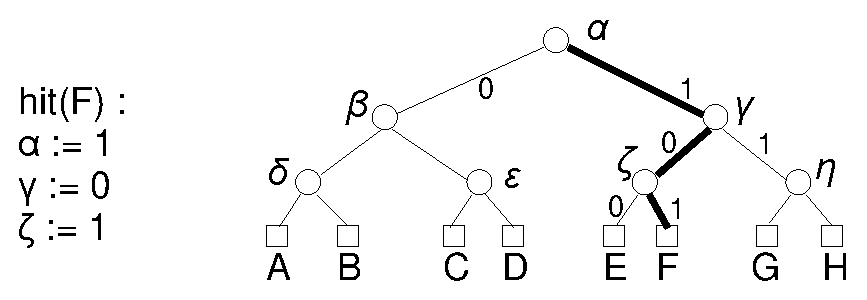
\includegraphics[width=0.7\textwidth]{2.theor/plruhit}\\
  \caption{Попадание для стратегия вытеснения \PseudoLRU
  (8-ассоциативная таблица)}\label{pseudo_lru_hit}
\end{figure}

На основании пометок вершин определяется и листовая вершина вытесняемой строки.
%Вытесняющий тег помещается в дереве на место вытесняемого.
Из корня дерева строится <<вытесняющий путь>> (он будет единственным), он приводит к вытесняемой строке. Начинает <<вытесняющий путь>> строиться из корневой вершины. Далее в <<вытесняющем пути>> исходящая дуга каждой вершины имеет пометку, противоположную пометке этой вершины. Т.е. если вершина помечена цифрой 0, значит дуга пути из этой вершины идет вправо, если вершина помечена цифрой 1 -- влево. Пример того, как определяется вытесняемая строка, показан на рис.~\ref{pseudo_lru_miss}. Цветом показаны пометки нелистовых вершин: черным
вершинам соответствует пометка 1, белым -- 0. В изображенном на рисунке дереве в качестве вытесняемой строки будет выбрана строка D, к которой ведет путь $\alpha-\beta-\varepsilon$.

\begin{figure}[h] \center
  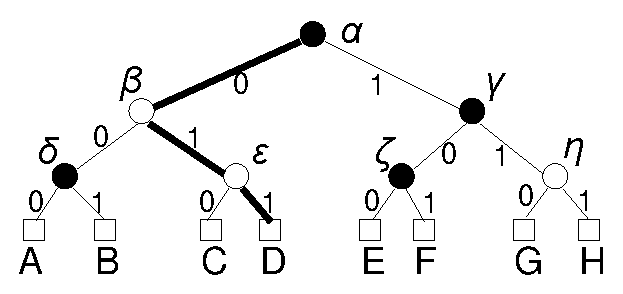
\includegraphics[width=0.5\textwidth]{2.theor/plrumiss}\\
  \caption{Определение вытесняемого элемента для стратегия вытеснения
  \PseudoLRU (8-ассоциативная таблица)}\label{pseudo_lru_miss}
\end{figure}


\subsubsection{Каноническое определение \PseudoLRU на битовой строке}

Для каждого региона хранится битовая строка $\beta$ длины $w{-}1$, где $w$ --
ассоциативность таблицы. Стратегия вытеснения определяется как процесс изменения
бит этой битовой строки.

Во многих книгах приводятся следующее определение стратегии
вытеснения \PseudoLRU для случая
$w=4$~\cite{FundamentalOfComputerOrganizationAndDesign} (в этом
случае для каждого региона выделяется 3 бита $B_1$, $B_2$ и $B_3$):
$$ \left[
  \begin{array}{c|ccc}
          & B_1 & B_2 & B_3 \\ \hline
    \pi_0 & 0 & 0 & \textsf{X} \\
    \pi_1 & 0 & 1 & \textsf{X} \\
    \pi_2 & 1 & \textsf{X} & 0 \\
    \pi_3 & 1 & \textsf{X} & 1 \\
  \end{array}
\right]
$$

Строки в регионе пронумерованы числами от 0 до $w{-}1$. При попадании на строку
региона с номером $i$ задействована строка матрицы, начинающаяся с $\pi_i$. Биты
$\beta$, напротив которых в строке матрицы находится \textsf{X}, не меняются.
Биты $\beta$, напротив которых в $i$'й строке находится число, принимают
значение, равное этому числу.

При промахе надо определить номер вытесняемой строки. Для этого используется
инвертированная форма той же матрицы (если элемент исходной матрицы был равен 0, то в инвертированной он равен 1; если в исходной равен 1, то в инвертированной равен 0; если в исходной равен \textsf{X}, то в инвертированной равен \textsf{X}):
$$
\left[
  \begin{array}{ccc|c}
    B_1 & B_2 & B_3 & \\ \hline
    1 & 1 & \textsf{X} & \rightarrow \pi_0 \\
    1 & 0 & \textsf{X} & \rightarrow \pi_1 \\
    0 & \textsf{X} & 1 & \rightarrow \pi_2 \\
    0 & \textsf{X} & 0 & \rightarrow \pi_3 \\
  \end{array}
\right]
$$

Выбирается строка матрицы, соответствующая текущему состоянию бит $B_1$,
$B_2$ и $B_3$, следующим образом: если напротив бита в строке матрицы находится число, бит
должен быть равен этому числу -- если напротив бита в строке матрицы
находится \textsf{X}, то соответствующий бит может иметь любое значение. Для любого набора значений $(B_1~B_2~B_3)$ подходящая строка матрицы всегда будет существовать и она будет единственной. Эта строка матрицы определяет вытесняемую строку региона.

Изменение $\beta$ обычно демонстрируют на бинарном дереве. Это то же дерево, что и в каноническом определении \PseudoLRU <<на бинарном дереве>>. $\beta$ составляется из пометок вершин дерева, начиная с корня и далее по слоям от левых к правым вершинам <<обходом в ширину>> (см. рис.~\ref{plru_bittree}).

\begin{figure}[h] \center
  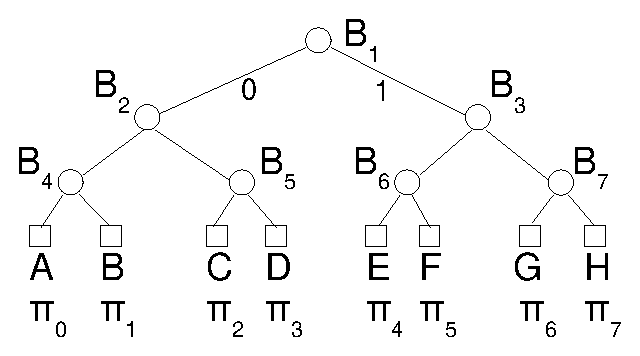
\includegraphics[width=0.5\textwidth]{2.theor/plru}\\
  \caption{Битовая строка в бинарном дереве}\label{plru_bittree}
\end{figure}

Формализованное описание для всех допустимых $w$ в литературе не
приводится. Однако в дальнейшем для формулирования и доказательства
утверждений про стратегию вытеснения \PseudoLRU такое описание будет
необходимо. Для $w=8$ изменение битовой строки будет задаваться следующей матрицей:
$$
\left[
  \begin{array}{c|ccccccc}
          & B_1 & B_2 & B_3 & B_4 & B_5 & B_6 & B_7 \\ \hline
    \pi_0 & 0 & 0 & \textsf{X} & 0 & \textsf{X} & \textsf{X} & \textsf{X} \\
    \pi_1 & 0 & 0 & \textsf{X} & 1 & \textsf{X} & \textsf{X} & \textsf{X} \\
    \pi_2 & 0 & 1 & \textsf{X} & \textsf{X} & 0 & \textsf{X} & \textsf{X} \\
    \pi_3 & 0 & 1 & \textsf{X} & \textsf{X} & 1 & \textsf{X} & \textsf{X} \\
    \pi_4 & 1 & \textsf{X} & 0 & \textsf{X} & \textsf{X} & 0 & \textsf{X} \\
    \pi_5 & 1 & \textsf{X} & 0 & \textsf{X} & \textsf{X} & 1 & \textsf{X} \\
    \pi_6 & 1 & \textsf{X} & 1 & \textsf{X} & \textsf{X} & \textsf{X} & 0 \\
    \pi_7 & 1 & \textsf{X} & 1 & \textsf{X} & \textsf{X} & \textsf{X} & 1 \\
  \end{array}
\right]
$$

Следующее утверждение~\ref{wMinus1PseudoLRU} дает алгоритм
преобразования битовой строки\\ $B_1,~B_2,~...,~B_{w{-}1}$ в результате
обращения в таблицу. В его формулировке будет применяться двоичное
разложение целых неотрицательных чисел от старших бит к младшим. Оно будет обозначаться для целого неотрицательного $x$ как $(x_1~x_2~...~x_n)_2$, где $x_i \in \{0, 1\}$ для $i = 1, 2, ..., n$, такие, что $x = x_n + 2{\cdot}x_{n-1} + 4{\cdot}x_{n-2} + \dots + 2^{n-1}{\cdot}x_1$. Например, 1 = (0 0 1)$_2$, 6 = (1 1 0)$_2$.

Обозначим символом $W$ выражение $\log_2 w$. По определению
стратегии вытеснения \PseudoLRU $W$ будет натуральным числом.

\begin{utv}[$(w{-}1)$-представление стратегии вытеснения
\PseudoLRU]\label{wMinus1PseudoLRU}При попадании по строке региона с номером $i = (i_1~i_2~\dots~i_W)_2$ происходит следующее изменение битовой строки $B_1,
B_2, ..., B_{w{-}1}$:

\parbox{0.3\textwidth}{
  $$ \begin{array}{l}
  B_{k_1} := i_1 \\
  B_{k_2} := i_2 \\
  B_{k_3} := i_3 \\
  ...\\
  B_{k_W} := i_W \\
  \end{array}$$
} \vline
\parbox{0.7\textwidth}{
  $$ \begin{array}{l}
  k_1 = (1)_2 \\
  k_2 = (1~i_1)_2 \\
  k_3 = (1~i_1~i_2)_2 \\
  ...\\
  k_W = (1~i_1~i_2~\dots~i_{W{-}1})_2 \\
  \end{array} $$
}
\\[1cm]

При промахе номер вытесняемой строки региона $j = (j_1~j_2~\dots~j_W)_2$ определяется следующим образом:

\parbox{0.3\textwidth}{
  $$ \begin{array}{l}
  i_1 = \neg B_{k_1} \\
  i_2 = \neg B_{k_2} \\
  i_3 = \neg B_{k_3} \\
  ...\\
  i_W = \neg B_{k_W} \\
  \end{array}$$
} \vline
\parbox{0.7\textwidth}{
  $$ \begin{array}{l}
  k_1 = (1)_2 \\
  k_2 = (1~\neg B_{k_1})_2 \\
  k_3 = (1~\neg B_{k_1}~\neg B_{k_2})_2 \\
  ...\\
  k_W = (1~\neg B_{k_1}~\neg B_{k_2}\dots\neg B_{k_{W{-}1}})_2 \\
  \end{array} $$
}
\\[0.5cm]

Кроме того при промахе делается такое же преобразование бит $B_1$, $B_2$, ..., $B_{w{-}1}$, как и в случае попадания на строку с номером $j$.
\end{utv}

Прямой проверкой нетрудно убедиться, что это утверждение верно для $w$ = 4 и 8.

\subsubsection{Определение \PseudoLRU на ветвях бинарного
дерева}\label{sec:PseudoLRUonBranches}

Здесь будет показано, как из канонических определений \PseudoLRU
получить формулировку \PseudoLRU с точки зрения одной строки региона~\cite{my_lomonosov_2010}
(в канонических определениях рассматривается весь регион целиком и
для него формулируются правила работы с последовательностью бит $B_1,
B_2, ..., B_{w{-}1}$ или пометками вершин бинарного дерева). Описываемое в этом разделе определение \PseudoLRU ранее не встречалось в литературе.

Сначала этот переход покажем в частном случае, на примере $w=4$. Первый шаг --- это
смена <<состояния>>: вместо последовательности бит $B_1, B_2, ...,
B_{w-1}$ будем рассматривать последовательность векторов бит
$\beta_0,~\beta_1,~\dots,~\beta_{w-1}$, каждый $\beta_i$ --- это вектор из $W$ бит. Каждый $\beta_i$ соответствует $i$'й листовой вершине бинарного дерева (см. рисунок~\ref{fig:plru_def_step1}). Попадание
меняет теперь атрибуты не внутренних вершин дерева $(B_1~B_2~B_3)$, а листовых $(\beta_0~...~\beta_3)$.
Каждый $\beta_i$ будет представляться списком длины $W$, обозначающим путь от
корня дерева к $i$'й листовой вершине: $\beta_0$ соответствует
($B_1$ $B_2$), $\beta_1$ соответствует ($B_1$ $\neg B_2$), $\beta_2$
соответствует ($\neg B_1$ $B_3$) и $\beta_3$ соответствует ($\neg
B_1$ $ \neg B_3$).\\[0.5cm]

\begin{figure}[h]
\parbox{0.2\textwidth}{ \centering
  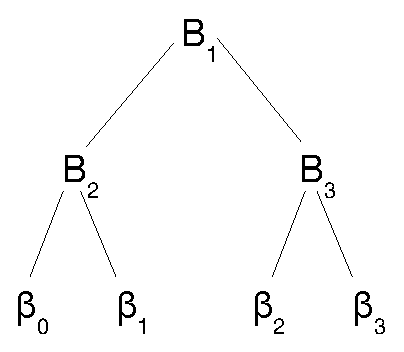
\includegraphics[width=0.2\textwidth]{1.review/btree}
}
\parbox{0.25\textwidth}{
$$ \left[
  \begin{array}{c|ccc}
          & B_1 & B_2 & B_3 \\ \hline
    \pi_0 & 0 & 0 & \textsf{X} \\
    \pi_1 & 0 & 1 & \textsf{X} \\
    \pi_2 & 1 & \textsf{X} & 0 \\
    \pi_3 & 1 & \textsf{X} & 1 \\
  \end{array}
\right]
$$
} $\stackrel{1}{\longrightarrow}$ %\vline
\parbox{0.4\textwidth}{
$$ \left[
  \begin{array}{c|cccc}
          & \beta_0 & \beta_1 & \beta_2 & \beta_3 \\ \hline
    \pi_0 & (0~0) & (0~1) & (1~\textsf{X}) & (1~\textsf{X}) \\
    \pi_1 & (0~1) & (0~0) & (1~\textsf{X}) & (1~\textsf{X}) \\
    \pi_2 & (1~\textsf{X}) & (1~\textsf{X}) & (0~0) & (0~1) \\
    \pi_3 & (1~\textsf{X}) & (1~\textsf{X}) & (0~1) & (0~0) \\
  \end{array}
\right]
$$
}
\caption{Смена состояния}\label{fig:plru_def_step1}
\end{figure}

Заметим, что получилась симметричная матрица. На пересечении $\pi_i$
и $\beta_j$ располагается вектор, задающий изменение $\beta_j$ (вектора в $j$'й
листовой вершине дерева) при попадании по строке региона, соответствующей $i$'й листовой вершине дерева. Назовем позицию $i \oplus j$ \emph{относительной позицией}
$i$ относительно $j$. Рассмотрим отдельно каждый столбец
получившейся матрицы (на рисунке~\ref{fig:plru_def_step2} до стрелки) и упорядочим строки столбцов в порядке увеличения относительных позиций (на рисунке~\ref{fig:plru_def_step2} после стрелки).

\begin{figure}[h]
\parbox{0.2\textwidth}{
$$ \left[
  \begin{array}{c|c}
          & \beta_0 \\ \hline
    \pi_0 & (0~0) \\
    \pi_1 & (0~1) \\
    \pi_2 & (1~\textsf{X}) \\
    \pi_3 & (1~\textsf{X}) \\
  \end{array}
\right]
$$
}\parbox{0.2\textwidth}{
$$ \left[
  \begin{array}{c|c}
          & \beta_1 \\ \hline
    \pi_0 & (0~1) \\
    \pi_1 & (0~0) \\
    \pi_2 & (1~\textsf{X}) \\
    \pi_3 & (1~\textsf{X}) \\
  \end{array}
\right]
$$
}\parbox{0.2\textwidth}{
$$ \left[
  \begin{array}{c|c}
          & \beta_2 \\ \hline
    \pi_0 & (1~\textsf{X}) \\
    \pi_1 & (1~\textsf{X}) \\
    \pi_2 & (0~0) \\
    \pi_3 & (0~1) \\
  \end{array}
\right]
$$
}\parbox{0.2\textwidth}{
$$ \left[
  \begin{array}{c|c}
          & \beta_3 \\ \hline
    \pi_0 & (1~\textsf{X}) \\
    \pi_1 & (1~\textsf{X}) \\
    \pi_2 & (0~1) \\
    \pi_3 & (0~0) \\
  \end{array}
\right]
$$
} $\stackrel{2}{\stackrel{\longrightarrow}{\pi^i_j \equiv \pi_{i
\oplus j}}}$

\parbox{0.24\textwidth}{
$$ \left[
  \begin{array}{c|c}
          & \beta_0 \\ \hline
    \pi^0_0 \equiv \pi_0 & (0~0) \\
    \pi^0_1 \equiv \pi_1 & (0~1) \\
    \pi^0_2 \equiv \pi_2 & (1~\textsf{X}) \\
    \pi^0_3 \equiv \pi_3 & (1~\textsf{X}) \\
  \end{array}
\right]
$$
}\parbox{0.24\textwidth}{
$$ \left[
  \begin{array}{c|c}
          & \beta_1 \\ \hline
    \pi^1_0 \equiv \pi_1 & (0~0) \\
    \pi^1_1 \equiv \pi_0 & (0~1) \\
    \pi^1_2 \equiv \pi_3 & (1~\textsf{X}) \\
    \pi^1_3 \equiv \pi_2 & (1~\textsf{X}) \\
  \end{array}
\right]
$$
}\parbox{0.24\textwidth}{
$$ \left[
  \begin{array}{c|c}
          & \beta_2 \\ \hline
    \pi^2_0 \equiv \pi_2 & (0~0) \\
    \pi^2_1 \equiv \pi_3 & (0~1) \\
    \pi^2_2 \equiv \pi_0 & (1~\textsf{X}) \\
    \pi^2_3 \equiv \pi_1 & (1~\textsf{X}) \\
  \end{array}
\right]
$$
}\parbox{0.24\textwidth}{
$$ \left[
  \begin{array}{c|c}
          & \beta_3 \\ \hline
    \pi^3_0 \equiv \pi_3 & (0~0) \\
    \pi^3_1 \equiv \pi_2 & (0~1) \\
    \pi^3_2 \equiv \pi_1 & (1~\textsf{X}) \\
    \pi^3_3 \equiv \pi_0 & (1~\textsf{X}) \\
  \end{array}
\right]
$$
}
\caption{Нумерация относительными позициями}\label{fig:plru_def_step2}
\end{figure}

После перехода к относительным позициям ($\pi^i_j$ -- это позиция
$\pi_j$ относительно $\pi_i$, т.е. $\pi_{i \oplus j}$) все столбцы получились одинаковыми.
Иными словами, \emph{алгоритм изменения порядка строк региона согласно стратегии
вытеснения \PseudoLRU на относительных позициях инвариантен
относительно абсолютной позиции вытесняемой строки}. Следующая теорема
формально доказывает этот факт.

Будем называть \emph{\PseudoLRU-ветвью позиции $i$} вектор
$(B_{k_1}^{\sigma_1}~B_{k_2}^{\sigma_2}~\dots~B_{k_W}^{\sigma_W})$,
в котором $k_1 = (1)_2, \sigma_1 = \neg i_1, \sigma_j = \neg i_j$, $k_j = (1~i_1~i_2~\dots~i_{j-1})_2$, $j = 2, 3, \dots, W$, $i = (i_1~i_2~\dots~i_W)_2$. Степени определены стандартным образом: $B^1 \equiv B, B^0 \equiv \neg B$. Например, \PseudoLRU-ветвью позиции 0 есть $(B_1~B_2~B_4~...)$. Каждой строке региона (т.е. каждой позиции строк региона) соответствует своя \PseudoLRU-ветвь. Каждое обращение изменяет все ветви некоторым образом, который не зависит от абсолютной позиции, а зависит от относительной:

\begin{theorem}[Инвариантность преобразования \PseudoLRU-ветвей относительными
позициями]\label{thm_pseudoLRU_invariant} \PseudoLRUInvariant
\end{theorem}
Доказательство теоремы приведено в приложении~\ref{sec:proofs}.

Доказанный факт позволяет сформулировать определение стратегии
вытеснения \PseudoLRU, сфокусированное не на изменении атрибутов строк всего
региона,
а на изменении атрибутов одной строки. На этом определении
будут базироваться применения предлагаемых методов генерации
ограничений для стратегии вытеснения \PseudoLRU.

\begin{utv}[формулировка \PseudoLRU на ветвях бинарного дерева]
Сопоставим некоторой произвольной строке региона вектор длины $W$. Каждое обращение к этой строке региона делает её вектор равным (0 0 ... 0). Строка региона является вытесняемой, если её вектор равен (1 1 ... 1).
Влияние других обращений определяется относительной позицией их
строки региона относительно позиции данной строки региона. Если относительная позиция
принадлежит области $[\frac{w}{2^k},~\frac{w}{2^{k-1}}), k =
1,2,...,W$, то первые $k{-}1$ элементов битового вектора становятся равными
0, $k$'й элемент вектора становится равным 1, остальные элементы
вектора не меняются. Если относительная позиция равна 0, то все элементы вектора становятся равными 0.
\end{utv}

Битовый вектор длины $W$ будет соответствовать пути из корня бинарного
дерева в листовую вершину, соответствующую данной строке региона.
Удобно представлять процесс изменения элементов бинарного вектора  в виде их
\emph{перекрашивания}. Про элементы битового вектора, равные 0,
будем говорить, что они покрашены в \emph{белый} цвет, а элементы вектора, равные 1, --- в\emph{черный}.

Говоря в терминах бинарного дерева из канонических определений \PseudoLRU, каждое обращение в регион изменяет пометки в нелистовых вершинах дерева. Каждой листовой вершине соответствует единственный в нее путь из корня дерева (та самая <<ветвь>>). Вершина дерева, входящая в ветвь, с точки зрения этой ветви будет <<белой>>, если пометка этой вершины совпадает с направлением дуги дерева из этой вершины. входящей в ветвь, <<черной>> --- если не совпадает. Вытесняется та строка региона, путь к которой полностью состоит из несоответствующих дуг по каноническим определениям, т.е. из черных вершин по новому определению. На рисунке~\ref{recolor}
изображен процесс перекрашивания ветви, ведущей в А, под действием
попадания в C (для сокращения показана только ветвь в А без
остальной части дерева). Так как путь из корня в C совпадает из
верхних двух вершин, то они перекрашиваются в белый цвет. Дуга из
третьей вершины пути в С не совпадает с дугой пути в А, поэтому
третья вершина перекрашивается в черный цвет. Остальные вершины
ветви остаются без изменений.

\begin{figure}[h] \center
  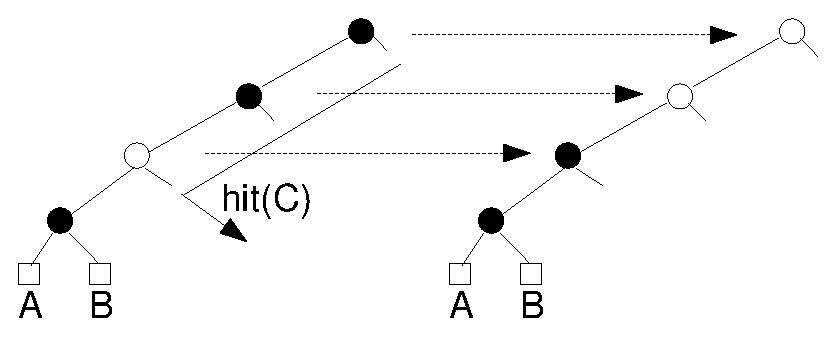
\includegraphics[width=0.8\textwidth]{1.review/recolor}\\
  \caption{Перекрашивание ветви в А}\label{recolor}
\end{figure}


Определение стратегии вытеснения \PseudoLRU на ветвях дерева
является связующим звеном между каноническим определением (например,
на битовой строке) и определением с помощью таблицы вытеснения,
поскольку ветвь -- это и есть двоичное разложение позиции, которая меняется точно так же, как и позиция в перестановке согласно таблице вытеснения.


%%%%%%%%%%%%%%%%%%%%%%%%%%%%%%%%%%%%%%%%%%%%%%%%%%%%%%%%%%%%%%%%%%%%

\section{Метод полезных обращений для записи стратегии вытеснения в виде ограничений}\label{sec:usefulness_functions}

%{\footnotesize В разделе рассматривается метод составления ограничений для
%описания стратегии вытеснения, для которой удается определить функционал
%вытеснения. Стратегия вытеснения описывается ограничением сверху на количество \emph{полезных} инструкций (т.е. помогающих вытеснению).
%В разделе приведены определения полезных инструкций и способы составления ограничений для трех
%наиболее часто используемых в микропроцессорах стратегий вытеснения -- \LRU, \FIFO и \PseudoLRU. Освещается понятие \emph{монотонного функционала вытеснения}, который является залогом более
%простой системы ограничений.}

В данном разделе процесс вытеснения будет представляться как изменение  системы функций, отображающих ключи в целые числа. Каждое обращение в таблицу изменяет значения функций по всем ключам\footnote{это напоминает изменение операций в рамках машин абстрактного состояния Ю.Гуревича~\cite{ASM}}. Пример процесса изменения значения функции для некоторого ключа изображен на рисунке~\ref{fig:graphic}.

\begin{figure}[h] \center
  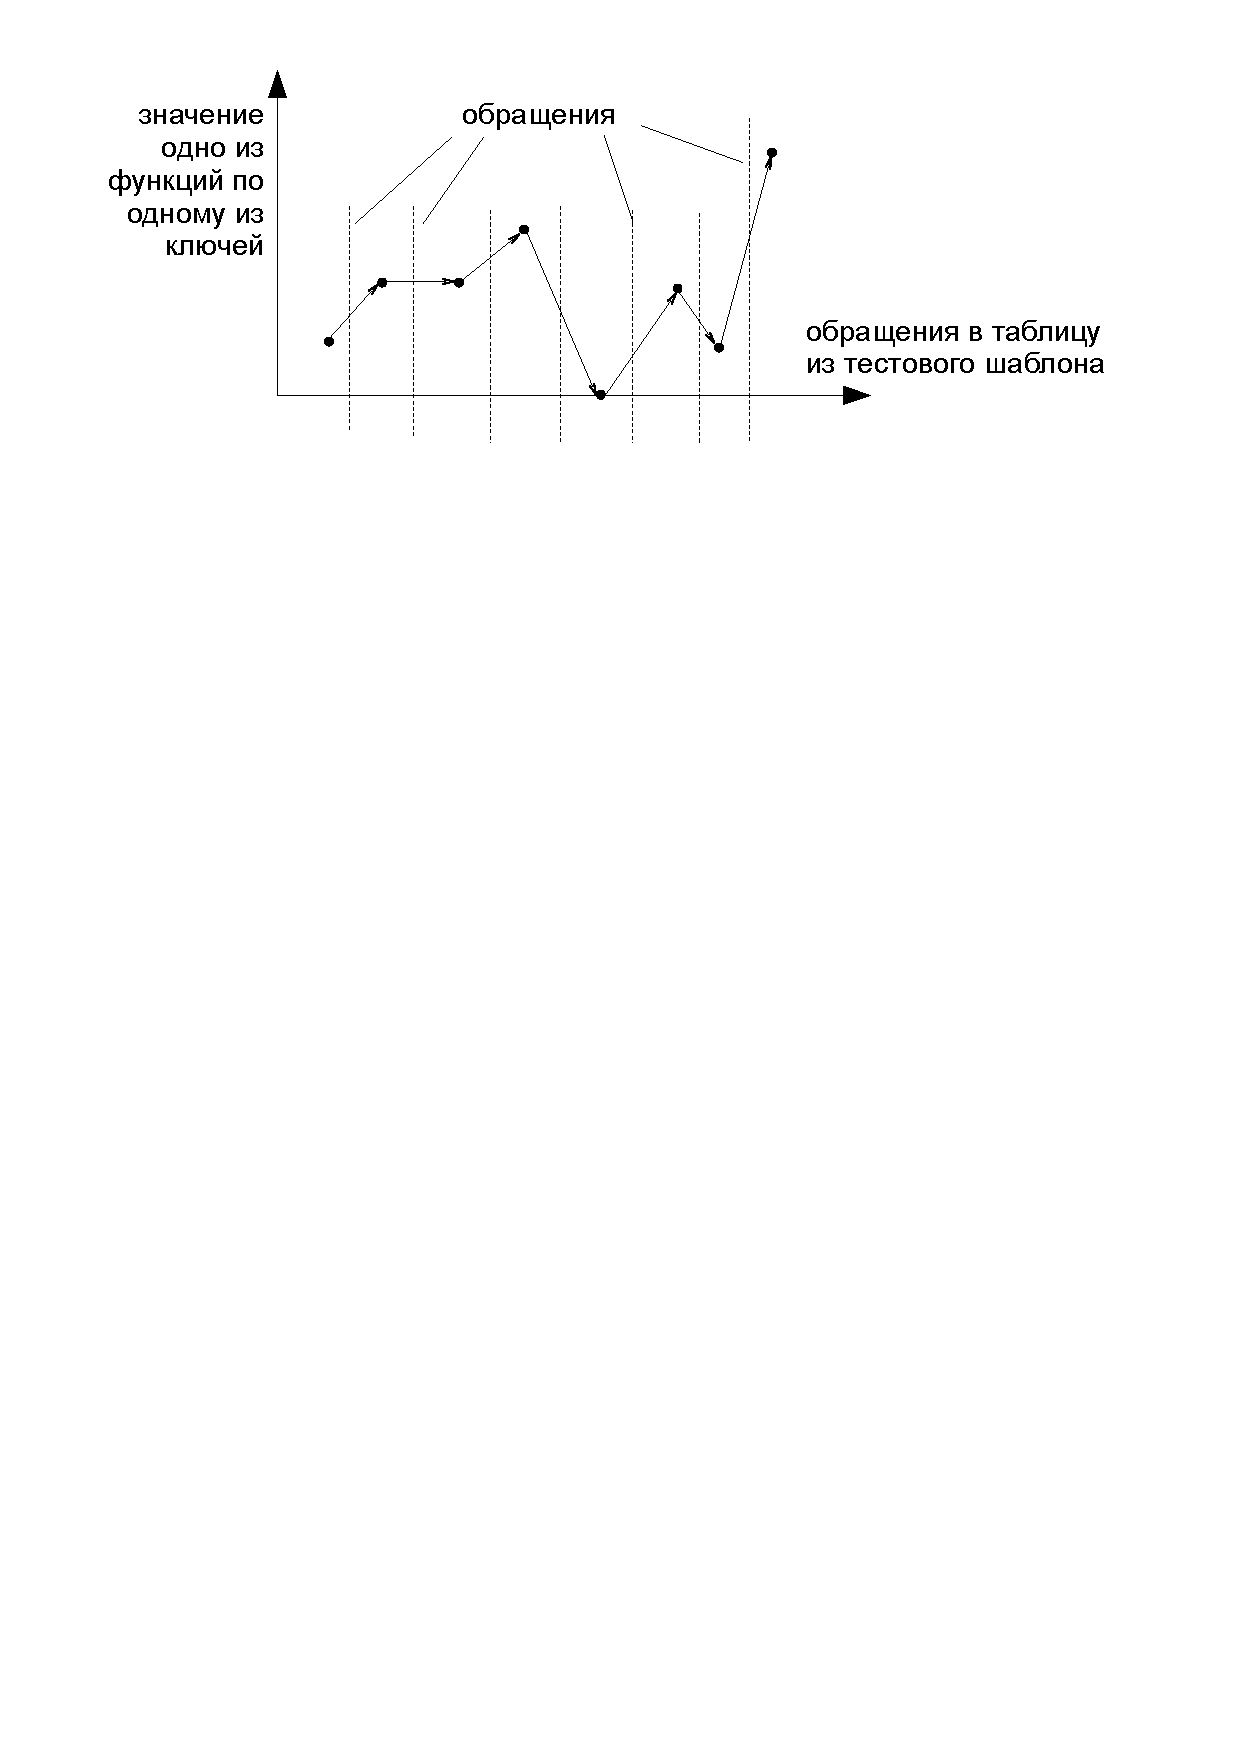
\includegraphics[width=0.7\textwidth]{2.theor/graphic}\\
  \caption{К определению стратегии вытеснения}\label{fig:graphic}
\end{figure}

Говоря формально, пусть $\alpha, \beta, \dots, \gamma$ --- одноместные функции,
отображающие ключи в целые числа. Для каждого обращения определены функции
изменения значений функций $\alpha, \beta, \dots, \gamma$ (если не сказано иное, будет предполагаться, что обращения осуществляются в один и тот же регион):
$$\parbox{2.5cm}{in-parallel\\forall keys x~}\left|\begin{array}{l}
\alpha(x) := A_I(k, \alpha, \beta, \dots, \gamma)\\
\beta(x) := B_I(k, \alpha, \beta, \dots, \gamma)\\
\dots\\
\gamma(x) := C_I(k, \alpha, \beta, \dots, \gamma)\\
\end{array}\right.
$$

Обновления значений функций $\alpha, \beta, \dots, \gamma$ выполняются одновременно. $I$ --- обращение в таблицу, $k$ --- ключ в этом обращении. Функции $A_I$, $B_I$, \dots, $C_I$ отражают влияние обращения по некоторому ключу на другой произвольный ключ. $x$ --- это ключ, за которым <<следим>> и условия вытеснения которого нас интересуют, а $k$ ---это ключ в очередном обращении из тестового шаблона.
Возможны следующие случаи (в качестве $x$ рассматривается произвольный ключ, не
обязательно <<находящийся>> в регионе):
\begin{itemize}
    \item в результате обращения по ключу $k$ ключ $x$ <<попадает>> в регион (т.е. в регион добавляется строка с ключом $x$);
    \item в результате обращения по ключу $k$ ключ $x$ <<вытесняется>> из региона (т.е. из региона удаляется строка с ключом $x$);
    \item в результате обращения по ключу $k$ <<состояние>> ключа $x$ в регионе не меняется.
\end{itemize}

%Этим ситуациям как раз и ставятся в соответствие классы значений функций $\alpha, \beta, \dots, \gamma$, а функции $A_I$, $B_I$, \dots, $C_I$ осуществляют переход между этими классами. Тем самым стратегия вытеснения будет описана в виде изменения таких <<счетчиков>> $\alpha, \beta, \dots, \gamma$.

%Формально это правило выражается следующим образом.
Будем называть функцию
$\alpha$, отображающую ключи в целые числа, \emph{функционалом вытеснения} для заданной стратегии вытеснения, если одновременно выполнены следующие свойства:
\begin{enumerate}
  \item существуют константы $\alpha_{min}$ и $\alpha_{max}$ такие, что
$\alpha_{min} \leqslant \alpha_{max}$;
  \item для любого ключа $x$ $\alpha_{min} \leqslant \alpha(x) \leqslant
\alpha_{max}$ тогда и только тогда, когда $x$ находится в регионе по определению
стратегии вытеснения (т.е. <<был помещен>> в регион и до сих пор не вытеснен);
  \item для любого ключа $k$ $A_I(k, \alpha,\beta,\dots,\gamma) (k) =
\alpha_{min}$;
  \item $\exists! \varphi: \mbox{~ключ~} \times \mathds{Z}^{n} \times \mbox{~ключ~} \times \mathds{Z}^{n} \rightarrow
\mathds{Z}$, где $n$ --- количество функций во множестве
$\{\alpha,\beta,\dots,\gamma\}$, такая, что для любого ключа $x$ $$A_I(k,
\alpha,\beta,\dots,\gamma)(x) \equiv \varphi(k, \alpha(k), \beta(k), \dots,
\gamma(k), x, \alpha(x), \beta(x), \dots, \gamma(x))$$ иными словами, в функции
изменения функционала вытеснения разрешается обращаться только к $k$ и тому ключу,
для которого определяется функционал вытеснения;
  \item $\exists!$ ключ $x^* : \alpha(x^*) = \alpha_{max}$;
  \item перед любым неуспешным обращением $\alpha(x^*) =
\alpha_{max}$ тогда и только тогда, когда $x^*$ есть <<вытесняемый>> ключ по
определению стратегии вытеснения (т.е. строка с ключом $x^*$ является
вытесняемой при данном обращении по определению стратегии вытеснения);
\end{enumerate}

Пример функционала вытеснения: $\alpha$ --- счетчик количества обращений к строке
для стратегии вытеснения \LRU. Обращение по тому же ключу делает $\alpha$
равным 1, по другому ключу --- увеличивает $\alpha$ на единицу. Вытесняемым
считается ключ, чей счетчик равен $w$ --- количеству строк в регионе. Проверим
определение функционала вытеснения:
\begin{enumerate}
    \item $\alpha_{min}$ = 1, $\alpha_{max}$ = $w$, $1 \leqslant w$;
    \item верно, что счетчик больше $w$ тогда и только тогда, когда $x$ не
находится в регионе; в противном случае, было бы возможно подряд успешно обратиться к
большему числу строк, чем хранится в регионе;
    \item по условию обращение по тому же ключу делает $\alpha$ равным 1, что
и есть $A_I(x;...)(x) = 1$;
    \item изменение одного счетчика производится независимо от изменений других счетчиков (хотя, конечно, все счетчики изменяются одновременно);
    \item такой $x^*$ существует, ибо в противном случае было бы возможно подряд успешно обратиться к большему числу строк, чем хранится в регионе; такой $x^*$ единственный, поскольку каждое обращение меняет каждый счетчик и в минимальное значение $\alpha$ изменяется лишь по единственному ключу.
\end{enumerate}

Пусть для стратегии вытеснения сформулирован функционал вытеснения. Будем называть
обращение по некоторому ключу \emph{полезным для вытеснения} ключа
$x$ (или просто, \emph{полезным}), если оно монотонно увеличивает функционал вытеснения по
ключу $x$ до максимального значения (см. рис.~\ref{useful}).\\

\begin{figure}[h] \center
  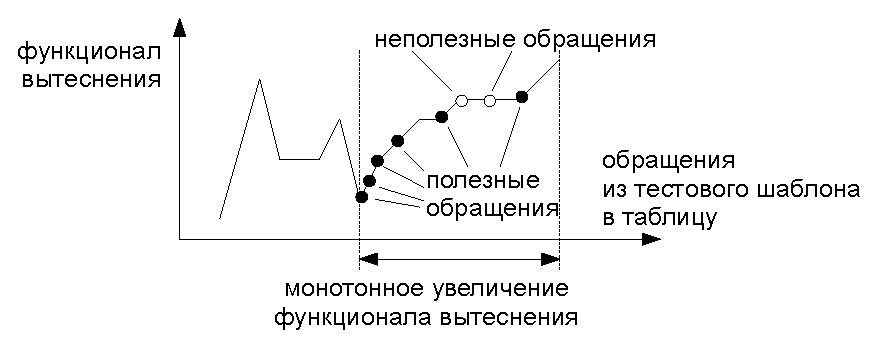
\includegraphics[width=0.6\textwidth]{2.theor/useful}\\
  \caption{К определению полезных обращений}\label{useful}
\end{figure}

Тогда вытеснение будет происходить в том случае, когда количество
полезных обращений превысит некоторое константное количество.
И вытеснение не будет происходить, если это количество не превысит некоторой константной верхней границы.

\emph{Формулой полезного обращения} будем называть предикат от вытесняемого ключа $k$ и региона $R$ и ключей и регионов предыдущих обращений, при которых это обращение будет полезным для вытеснения ключа $k$ из региона $R$.

Тем самым ограничение (constraint) <<быть вытесненным>> представимо в виде
ограничения сверху на <<сумму>> формул полезных обращений по всем предыдущим обращениям: $\sum_{i=1}^n [u_x(k_i)] < N$, где $u_x(k_i)$ -- формула полезного обращения по ключу $k_i$ для ключа $x$ в полностью ассоциативной таблице, для остальных таблиц будут указываться регионы обращений: $u_{x,r}(k_i, r_i)$.

Формулы полезных обращений, как и функционалы вытеснения, не являются единственными. Например, для стратегии вытеснения \LRU возможны следующие две различные формулы полезных обращений (далее для одной из них будет формально показано, что она действительно задает полезные обращения) (формулы приведены для случая полностью ассоциативной таблицы):
\begin{itemize}
  \item $u_x(x_i) \equiv (x \notin \{x_i, x_{i+1}, ..., x_n\} \wedge
\bigwedge\limits_{j=1}^{i-1} (x \in \{x_j, x_{j+1}, ..., x_{i-1}\} \vee x_j
\neq x_i))$ -- обращение считается полезным, если оно расположена после
последнего обращения к $x$ и с того момента является первым обращением к своему
ключу; нетрудно заметить, что это в чистом виде определение \LRU, изображенное на рисунке~\ref{fig:lru1}: обращение по ключу $x_j$, который расположен после ключа $x$, передвигает $x$ к концу вектора, за концом происходит вытеснение; первые обращения по ключам после последнего обращения к $x$ -- это и есть именно те обращения, где $x$ сдвигается к концу; иначе говоря, полезное обращение сдвигает $x$ к концу, приближая его к вытеснению;
  \item $u_x(x_i) \equiv (x \notin \{x_i, x_{i+1}, ..., x_n\} \wedge x_i \notin
\{x_{i+1}, x_{i+2}, ..., x_n\})$ -- обращение считается полезным, если оно
расположено после последнего обращения к $x$ и является последним обращением к
своему ключу перед финальным обращением к $x$; т.е. в таблице хранятся некоторые ключи, есть некоторый ключ $x$, есть последовательность других обращений (их
ключи обозначены как  $x_i$, ..., $x_n$), полезными будут лишь последние к ним обращения (среди $x_i$, ..., $x_n$ могут быть равные), т.е. все полезные обращения вместе образуют (по разу) все различные ключи.
\end{itemize}

Тем самым, метод полезных обращений состоит в следующем:
\begin{enumerate}
  \item выделить функционал вытеснения $\alpha$;
  \item выделить определение полезной инструкции;
  \item записать формулу полезного обращения $u_{x,r}(x_i, r_i)$ для обращения с ключом $x$ и регионом $r$;
  \item определить $\alpha_{max}$;
  \item составить ограничение для свойства <<$x$ вытеснен>> в виде
$\sum\limits_{i=1}^n u_{x,r}(x_i, r_i) > \alpha_{max}$ и для свойства <<$x$ не
вытеснен>> в виде $\sum\limits_{i=1}^n u_{x,r}(x_i,r_i) \leqslant \alpha_{max}$.
\end{enumerate}

Ключевой вопрос при применении метода полезных обращений --- это выбор
функционала вытеснения. От него в том числе будет зависеть сложность функции
полезности и генерируемых ограничений.

 Функционал вытеснения может быть получен из таблицы вытеснения
(policy table). А именно, если вытеснение происходит с позиции с максимальным
номером (т.е. в последней строке отсутствует число $w{-}1$), а в результате
попадания ключ переносится в самое начало (т.е. второй столбец имеет вид (0 1 2
... $w{-}1$ $m$)$^T$ ). Тогда $\alpha$ --- это позиция ключа в перестановке,
$\alpha_{min}$ = 0, $\alpha_{max} = w{-}1$. Этими свойствами, например, обладают
таблицы вытеснения \LRU (см.рис.~\ref{fig:PolicyTableLRU8}) и
\PseudoLRU~\cite{policy_tables}.

%В отличие от метода диапазонов вытеснения при использовании функций полезности не происходит выделение участка тестового шаблона, непосредственно влияющего на вытеснение. Считается, что это влияние начинается с момента появления строки в таблице. Другое дело, что одни инструкции влияют на ее вытеснение (это и есть <<полезные>> инструкции), а другие -- нет.


\subsection{Метод полезных обращений для стратегии вытеснения \LRU}

\LRU (Least Recently Used) --- это стратегия вытеснения,
определяющая вытесняемые данные как наименее используемые. Она
эффективна для алгоритмов, обладающих свойством локальности данных,
т.е. чаще использующих те данные, к которым недавно происходило
обращение. Эта стратегия используется, например, в микропроцессорах
архитектуры MIPS~\cite{mips64II}.

Стратегия вытеснения \LRU обычно определяется с использованием
счетчиков обращений. Для каждой строки таблицы
вводится счетчик обращений к ней. Каждое обращение увеличивает
счетчик. Счетчик вытесняющей строки на единицу больше максимального счетчика невытесняемых строк. Вытесняемой в регионе будет строка с минимальным счетчиком его строк.
%Поскольку границы значений счетчика неизвестны, формулирование
%функционала вытеснения на основе счетчика провести сложно.

Другой способ описания \LRU основан на введении порядка на строках региона (т.е.
регион представляется вектором строк). После каждой инструкции элементы этого вектора переупорядочиваются, \emph{переставляются}, согласно следующим правилам (см.рис.~\ref{fig:lru1}):
\begin{itemize}
\item при попадании соответствующая строка перемещается в начало, строки, которые расположены левее этой, сдвигаются на одну позицию вправо;
\item при промахе вытесняется последняя строка, в начало вставляется вытесняющая.
\end{itemize}

\begin{figure}[h] \center
  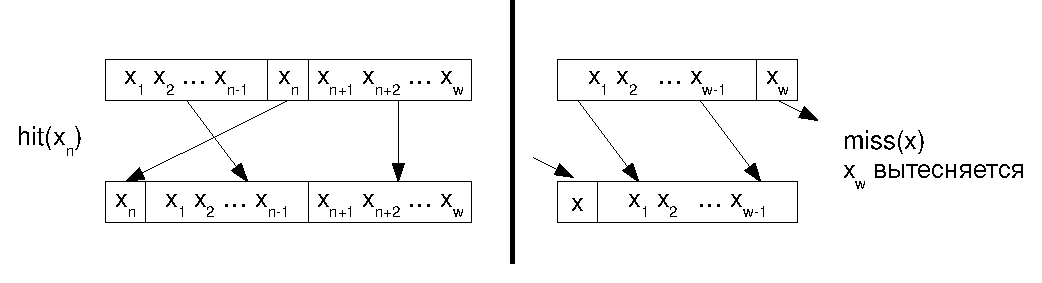
\includegraphics[width=0.6\textwidth]{2.theor/lru1}\\
  \caption{Стратегия вытеснения \LRU (w --- ассоциативность) на
перестановках}\label{fig:lru1}
\end{figure}

Позиция строки, ее индекс, в таком векторе ограничена, единственна, ее изменение допускает представление, независимое от других ключей. Тем самым \emph{<<позиция>> ключа является функционалом вытеснения}.

Функция изменения этого функционала выглядит следующим образом:\\

\parbox{0.5\textwidth}{ \tt
$A_{\mbox{hit}}(k, \alpha)(x) \equiv$\\
if $\alpha(x) > w$ then $\alpha(x)$\\
elsif $\alpha(k) > \alpha(x)$ then $\alpha(x)+1$\\
elsif $\alpha(k) = \alpha(x)$ then $1$\\
else $\alpha(x)$ endif%
}\parbox{0.5\textwidth}{\tt
$A_{\mbox{miss}}(k, \alpha)(x) \equiv$\\
if $k = x$ then $1$\\
elsif $\alpha(x) > w$ then $\alpha(x)$\\
else $\alpha(x) + 1$ endif}\\

Полезным будет считаться обращение, увеличивающее позицию, т.е.
переставляющее соответствующий ключ к концу. Такими обращениями являются все
промахи (поскольку они вытесняют последнюю строку вектора с передвижением всех остальных на одну позицию к концу, т.е. будет передвинута и строка с ключом $x$) и
попадания к строкам, находившимся ближе к концу, чем $x$ (потому как при попадании они передвинутся в самое начало, а все строки от начала и до них сдвинутся на одну
позицию к концу, в том числе и $x$).

Осталось выразить эту идею в виде ограничений~\cite{my_ewdts_2009}.
Учет полезных обращений начинается уже в инициализирующей последовательности,
тем самым необходимо будет сформулировать формулы полезных обращений и для
инициализирующих обращений.

Следующая теорема описывает функцию полезности для \LRU ($m$ --- количество
инициализирующих инструкций):

\begin{theorem}[Выражение свойства <<быть вытесненным>> для \LRU]\label{correct_mirror_LRU} \LRUusefuls
\end{theorem}

\begin{proof}
По определению стратегии вытеснения \LRU <<$k$ не вытеснен из региона $R$ согласно определению на перестановках>> эквивалентно тому, что после последнего обращения к $k$ в $R$ происходит не более $w$ обращений по различным ключам в регион $R$. Несложно убедиться, что это количество выражается следующей формулой: $$|\{s_i| R = R(s_i) \wedge s \notin \{s_i, ..., s_{m+n}\}\}|$$
Однако это же число можно записать другим образом, чтобы исключить повторения одинаковых $s_i$:
$$|\{s_i| R = R(s_i) \wedge s \notin \{s_i, ..., s_{m+n}\} \wedge s_i \notin \{s_{i+1}, ..., s_{m+n}\}\}|$$

Ввиду конечности последовательности $\langle s_i, ..., s_{m+n}\rangle$ в нем всегда найдется последнее вхождение $s_i$ --- множество последних вхождений всех элементов списка равно множеству всех элементов списка.

Представленная мощность множества и есть требуемая сумма.
\end{proof}

Из теоремы~\ref{correct_mirror_LRU} следует система ограничений для
описания обращений по ключу $k_i$ в регион $R_i$ согласно методу полезных обращений для \LRU: \begin{itemize}
\item для hit($k_i, R_i$):
$$
\left\{\begin{array}{l} (k_i||R_i) \in \{(t_1||r_1), ..., (t_m||r_m), (k_1||R_1),
..., (k_{i-1}||R_{i-1})\}\\
\sum\limits_{j=1}^m [u_{k_i,R_i}(t_j||r_j)] + \sum\limits_{j=1}^{i-1} [u_{k_i,R_i}(k_j||R_j)] < w\\
\{(t_1||r_1), ..., (t_m||r_m)\} - \mbox{все разные}\\
\end{array} \right.
$$
\item для miss($k_i, R_i$):
$$
\left\{\begin{array}{l} (k_i||R_i) \in \{(t_1||r_1), ..., (t_m||r_m), (k_1||R_1),
..., (k_{i-1}||R_{i-1})\}\\
\sum\limits_{i=1}^m [u_{k_i,R_i}(t_j||r_j)] + \sum\limits_{j=1}^{i-1} [u_{k_i,R_i}(k_j||R_j)]
\geqslant w\\
\{(t_1||r_1), ..., (t_m||r_m)\} - \mbox{все разные}\\
\end{array} \right.
$$
\end{itemize}


%Для этого удобно использовать утверждение~\ref{hit_miss_human}. Символом
%$\lambda_\delta$ будет обозначаться элемент начального
%состояния таблицы с индексом $\delta$ по порядку \LRU, $1 \leqslant \delta \leqslant w$. Индекс 1 обозначает самый молодой элемент, индекс $w$ обозначает самый старый элемент.
%
%Применение полезностей эффективно в том случае, когда домен имеет
%небольшой размер. В этом случае можно перебрать все элементы
%домена (это и будут $\lambda_\delta$) и составить для них свои
%полезности, причем для каждого элемента будет известен индекс по
%порядку \LRU ($\delta$). Ограничение, описывающее стратегию
%вытеснения, будет при этом иметь вид дизъюнкции по элементам домена.
%
%Если вытесняемый элемент был в начальном состоянии (пусть это
%$\lambda_\delta$) и к нему не было обращений, то для его вытеснения
%необходимо $w-\delta + 1$ полезных инструкций, потому что столько
%раз надо подвинуть элемент с индексом $\delta$ в \LRU-списке в
%сторону к концу (к элементам с индексом $w$), чтобы он вышел за
%границу списка (иными словами, чтобы он был вытеснен).
%
%Если вытесняемый элемент был в начальном состоянии и к нему было
%обращение, то для его вытеснения необходимо $w$ инструкций, так как
%во время обращения элемент был поставлен в самое начало \LRU-списка.
%То же справедливо для внесенных в кэширующий буфер новых тегсетов --
%чтобы их вытеснить, надо так же $w$ полезных инструкций, чтобы
%переместить их к концу \LRU-списка.
%
%В таблице~\ref{hit_miss_table} приведены все функции полезности для
%кэш-попаданий и кэш-промахов. Доказательство корректности приведенных
% в ней формул (т.е. доказательство того, что эти формулы действительно
% описывают \LRU) важны, но не представляют самостоятельного результата.
%Поэтому они были вынесены за пределы основной части диссертации и
%находятся в приложении~\ref{sec:proofs}.

В некоторых случаях количество ограничений удается сократить, используя следующую эвристику для ограничения вида $\sum_{i=1}^n a_i \leqslant C$:
\begin{itemize}
    \item если $C > n$, то его не включать в конъюнкцию;
    \item если $C < 0$, то вся конъюнкция с этим ограничением несовместна;
    \item если $C = 0$, то его сразу расписать в конъюнкцию ограничений
$a_i = 0$ для каждого $i$ от 1 до $n$;
    \item если $C = n$, то его сразу расписать в конъюнкцию ограничений
$a_i = 1$ для каждого $i$ от 1 до $n$.
\end{itemize}

Аналогично с ограничениями вида $\sum_{i=1}^n a_i \geqslant C$.


\subsection{Метод полезных обращений для стратегии вытеснения \FIFO}

\FIFO (First-In First-Out) -- это стратегия вытеснения, определяющая
вытесняемые данные согласно принципу очереди FIFO. Например, в
микропроцессоре PowerPC 970FX вытеснение из небольшого буфера,
хранящего последние преобразованные эффективные адреса в физические,
D-ERAT, происходит согласно \FIFO~\cite{PowerPC970FXUserManual}.

Стратегия \FIFO допускает описание на основе порядка на строках
региона (т.е. регион представляется вектором строк-элементов). После каждого
обращения строки вектора переупорядочиваются, \emph{перставляются}, согласно следующим правилам
(см.рис.~\ref{fifo1}):
\begin{itemize}
\item при попадании порядок строк не меняется;
\item при промахе вытесняется последняя строка, в начало вставляется вытесняющая строка.
\end{itemize}

\begin{figure}[h] \center
  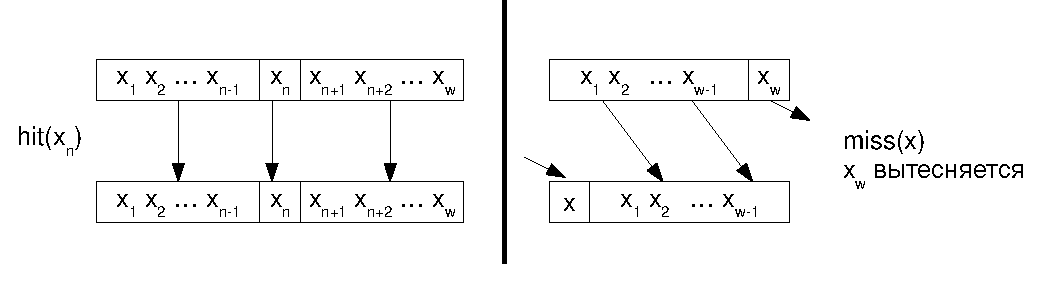
\includegraphics[width=0.6\textwidth]{2.theor/fifo1}\\
  \caption{Стратегия вытеснения \FIFO (w --- ассоциативность
таблицы)}\label{fifo1}
\end{figure}

Отличие от \LRU лишь в том, что при \FIFO не происходит перестановки
строк при возникновении попадания. Поэтому таблица
вытеснения~\cite{policy_tables} для стратегии вытеснения \FIFO будет
выглядеть так, как изображено на рисунке~\ref{fifo_policy_table}.

\begin{figure}[h]
$$
  \left[
    \begin{array}{c|cccccc}
      \pi_0 & 0 & 1 & 2 & 3 & \dots & w{-}1 \\
      \pi_1 & 0 & 1 & 2 & 3 & \dots & w{-}1 \\
      \pi_2 & 0 & 1 & 2 & 3 & \dots & w{-}1 \\
      \vdots &  &  &  & & & \\
      \pi_{w-1} & 0 & 1 & 2 & 3 & \dots & w{-}1 \\
      \pi_m & m & 0 & 1 & 2 & \dots & w{-}2 \\
    \end{array}
  \right]
$$
\caption{Таблица вытеснения для \FIFO}\label{fifo_policy_table}
\end{figure}

Формулы полезных обращений для \FIFO будем строить также на основе уже сформулированных и обоснованных формул для \LRU.

%Кроме того все инструкции с попаданиями, поскольку они не влияют на вытеснение, можно вообще исключить из ограничений.

Таким образом система уравнений для описания обращений по ключу $k$ в регион $R$
согласно методу полезных обращений для \FIFO выглядит следующим образом:
\begin{itemize}
\item для hit($k_i, R_i$):
$$
\left\{\begin{array}{l} (k_i||R_i) \in \{(t_1||r_1), ..., (t_m||r_m), (k_1||R_1), ..., (k_{i-1}||R_{i-1})\}\\
\sum\limits_{j=1}^m [u_{k_i,R_i}(t_j||r_j)] + \sum\limits_{j=1..{i-1}:(k_j,R_j)\mbox{~--miss}} [u_{k_i,R_i}(k_j||R_j)] < w\\
\{(t_1||r_1), ..., (t_m||r_m)\} - \mbox{все разные}\\
\end{array} \right.
$$
\item для miss($k_i, R_i$):
$$
\left\{\begin{array}{l} (k_i||R_i) \in \{(t_1||r_1), ..., (t_m||r_m), (k_1||R_1), ..., (k_{i-1}||R_{i-1})\}\\
\sum\limits_{j=1}^m [u_{k_i,R_i}(t_j||r_j)] + \sum\limits_{j=1..{i-1}:(k_j,R_j)\mbox{~--miss}} [u_{k_i,R_i}(k_j||R_j)] \geqslant w\\
\{(t_1||r_1), ..., (t_m||r_m)\} - \mbox{все разные}\\
\end{array} \right.
$$
\end{itemize}

$$u_{k_i,R_i}(s_j) \equiv ((k_i||R_i) \notin \{s_j, ..., s_{m+n}\} \wedge R_i = R(s_j) \wedge s_j \notin\{s_{j+1},..., s_{m+n}\})$$
$s \equiv \langle (t_1||r_1), ..., (t_m||r_m), (k_1||R_1), ..., (k_n||R_n)\rangle$, $R(s_i)$ --- вторая компонента $s_i$ (регион).


\subsection{Метод полезных обращений для стратегии вытеснения \PseudoLRU}

Для определения функционала вытеснения воспользуемся определением\\\PseudoLRU <<на ветвях бинарного дерева>> (см. раздел~\ref{sec:PseudoLRUonBranches}). А именно, определение того, вытеснен ли ключ $k$ в регионе $R$, будет вестись на основе атрибутов вершин пути от корня дерева к  листу, соответствующему $k$. Эти вершины могут быть белыми (им сопоставлено число 0) или чёрными (им сопоставлено число 1). Обращение по другому ключу $k_i$ в этом же регионе перекрашивает некоторые вершины этого пути. А именно, при следовании от корня к листу сначала часть вершин перекрашивается в белый цвет, затем одна вершина красится в черный цвет, остальные вершины не перекрашиваются. Если $k_i = k$, то все вершины ветви красятся в белый цвет.

  \begin{figure}[h] \center
  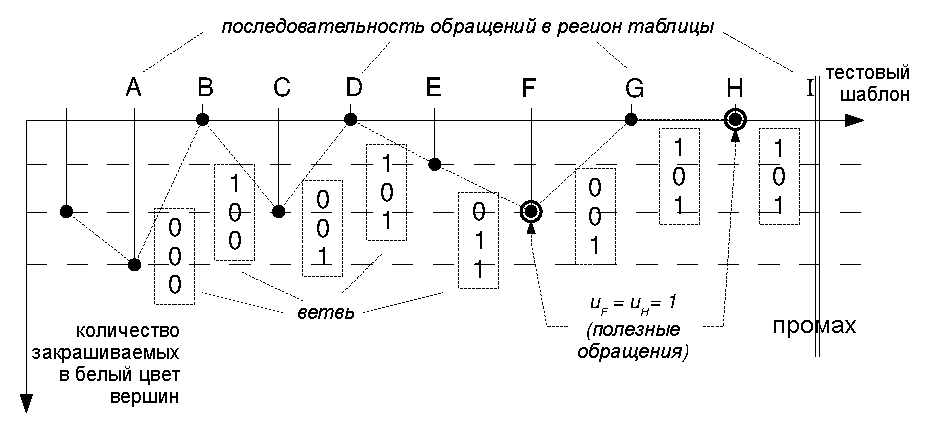
\includegraphics[width=\textwidth]{2.theor/plru_usefl_exmp}
  \caption{Перекрашивание ветви последовательностью обращений}\label{fig:plru_exmp_vytesn}
  \end{figure}

На рисунке~\ref{fig:plru_exmp_vytesn} изображен пример процесса перекрашивания для \\8-ассоциативной таблицы. В этом примере рассматривается ветвь, ведущая в строку, к которой происходит обращение А. После обращения к своей же строке вся ветвь становится белой: линия из А в В помечена (0 0 0)$^T$. Чем <<глубже>> по оси ординат происходит обращение, тем <<глубже>> становится белой ветвь (значение по оси ординат означает количество подряд вершин ветви, начиная с первой (самой верхней в векторах на рисунке), которые становятся равными нулю, а следующая за ней вершина, если она существует, становится равной единице, остальные вершины не меняются). Обращение В самое <<мелкое>>, оно лишь меняет первую вершину ветви, делая ее чёрной. Следующее обращение, С, перекрашивает 2 вершины в белый цвет (в том числе и ту вершину, которую только что обращение В покрасило в чёрный цвет) и 1 вершину в чёрный цвет. И так далее.

Обратим внимание на обращения F и H. Вершины, которые они закрашивают в чёрный цвет, сохраняют свой цвет до промаха, в котором будет определяться, вытеснять ли данную строку. Это происходит потому, что все следующие обращения происходят с закрашиванием меньшего числа вершин, чем F и H. В качестве функционала вытеснения рассмотрим количество таких обращений, как F и H, т.е. таких, после которых обращения закрашивают меньшее число вершин: самое большое число таких вершин есть длина ветви, самое малое - ноль (обращение А), изменений одной ветви определяется без отсылок к другим ветвям, вытеснение происходит тогда и только тогда, когда количество чёрных вершин равно длине ветви.

%Например, представленный на рисунке~\ref{fig:plru-useful} шаблон успевает
% покрасить 5 вершин ветви в черный цвет.
%
%\begin{figure}[t] \center
%  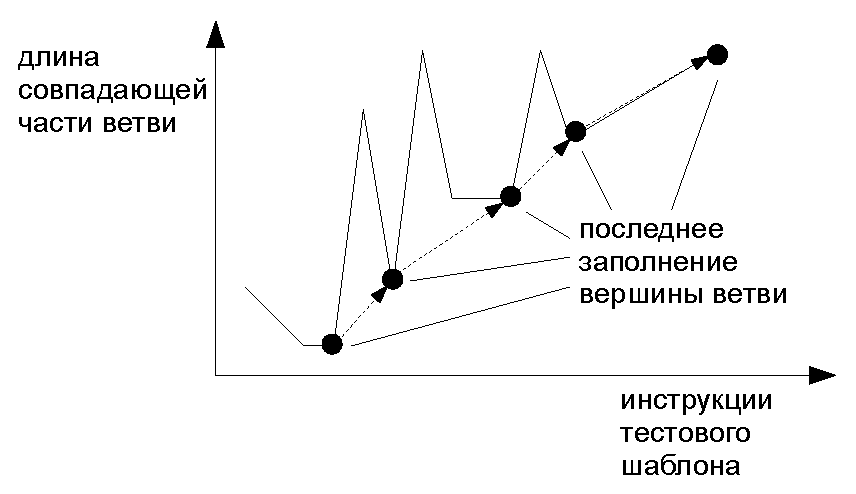
\includegraphics[width=0.6\textwidth]{2.theor/plru-useful}\\
%  \caption{Заполнение ветви черными вершинами в стратегии вытеснения
%  \PseudoLRU}\label{fig:plru-useful}
%\end{figure}

\begin{utv}
Обращение $I$ считается полезным в случае стратегии вытеснения \PseudoLRU, если все последующие обращения (до промаха, в котором вся ветвь будет чёрной) затрагивают только те вершины ветви, которые расположены выше вершины, перекрашиваемой инструкцией $I$ в черный цвет.
\end{utv}

Для вытеснения нужно не менее $\log_2 w$ полезных обращений (длина ветви). Далее выражение $\log_2 w$ будет обозначаться буквой $W$.

%Отличие этого функционала вытеснения от функционала для \LRU является \emph{немонотонность}. Это означает, что полезные инструкции надо считать для каждого промаха заново ---
%инструкции между двумя соседними промахами могут <<забелить>>
%несколько вершин ветви, что уменьшит функционал вытеснения
%(см.рис.~\ref{nonmonotonic}). Метрика для \LRU является монотонной,
%потому что инструкции между промахами не могут уменьшить функционал вытеснения -- либо не меняют, либо увеличивают ее, сдвигая ключ к концу вектора \LRU (см. рис.~\ref{monotonic}).
%
%%Таким образом, ограничение, описывающее стратегию вытеснения
%%\PseudoLRU, будет представлено дизъюнкцией ограничений по всем
%%предыдущим кэш-промахам.
%
%\begin{figure}[h] \center
%  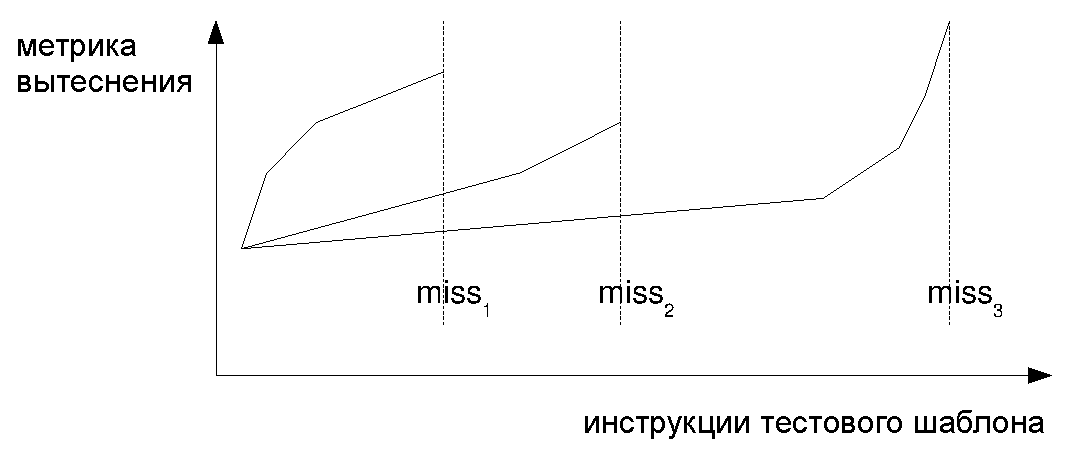
\includegraphics[width=0.6\textwidth]{2.theor/nonmonotonic}\\
%  \caption{Немонотонный функционал вытеснения}\label{nonmonotonic}
%\end{figure}
%
%\begin{figure}[h] \center
%  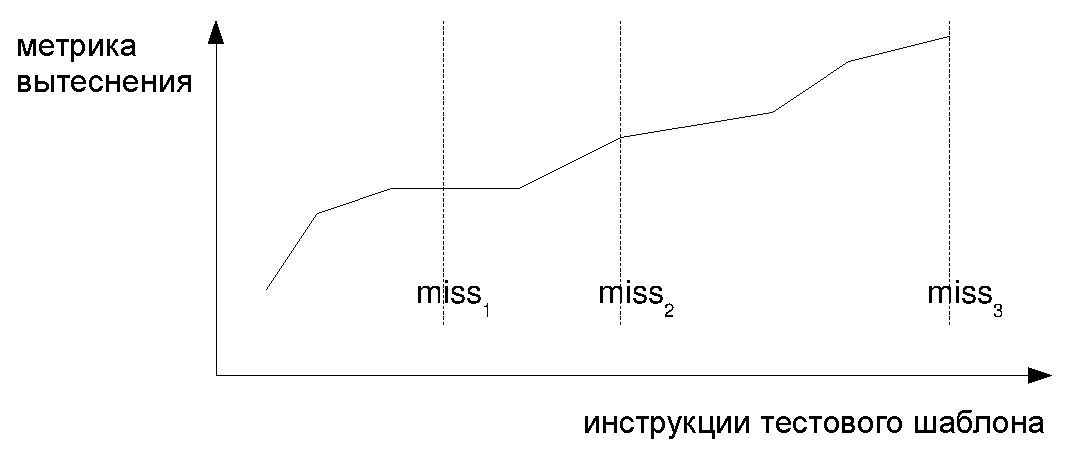
\includegraphics[width=0.6\textwidth]{2.theor/monotonic}\\
%  \caption{Монотонный функционал вытеснения}\label{monotonic}
%\end{figure}

Осталось записать формулу полезного обращения для \PseudoLRU в виде ограничений. Определимся с набором переменных. Каждому обращению в таблицу будут соответствовать следующие переменные:
\begin{itemize}
  \item ключ $k_i$;
  \item регион $R_i$;
  \item позиция $\pi_i$ (определение см. в разделе~\ref{sec:PseudoLRUonBranches}), $\pi_i \in \{0..w{-}1\}$;
  \item позиция $\pi'_i$ в момент последнего обращения перед данным (только для неинициализирующих обращений).
\end{itemize}

Обращение по ключу $k_i$ в регион $R_i$ на позицию $\pi_i$ будет полезным для вытеснения ключа $k_{n+1}$ в регионе $R_{n+1}$ ($i < n+1$) с позицией в момент последнего обращения $\pi'_{n+1}$, если выполнены все следующие условия (ниже будет доказано, что это определение соответствует стратегии вытеснения \PseudoLRU):
\begin{enumerate}
  \item <<$i$'е>> обращение происходит после последнего обращения к $k_{n+1}$ в $R_{n+1}$ перед $(n+1)$'м обращением;
  \item <<$i$'е>> обращение происходит в тот же регион, что и $R_{n+1}$;
  \item <<$i$'e>> обращение происходит до ближайшего повторного обращения на позиции $\pi'_{n+1}$;
  \item все обращения после <<$i$'го>> до ближайшего повторного обращения на позиции $\pi'_{n+1}$ просходит без закрашивания той вершины, которую красит <<$i$'e>> обращение.
\end{enumerate}

В момент последнего обращения по ключу $k_{n+1}$ в $R_{n+1}$ ветвь к нему становится целиком белой и начинается процесс вытеснения. Последующие инструкции перекрашивают эту ветвь до тех пор, пока не встретится обращение с промахом на той же позиции, которая была в момент последнего обращения к $k_{n+1}$ в $R_{n+1}$. К этому моменту вся ветвь должна стать чёрной, а после этого обращения ветвь вновь становится белой, но эта ветвь уже относится к другому ключу (тому, который вытеснил $k_{n+1}$).

Поясню этот момент с другой стороны. Рассматривая успешность очередного обращения к некоторому ключу, ищем ближайшее предыдущее обращение к тому же ключу (обращение А на рисунке~\ref{fig:plru_exmp_vytesn}). Обращения, идущие после этого <<предыдущего>>, либо должны вытеснить соответствующий ключ (если речь идёт о неуспешном обращении), либо не должны вытеснить (если --- об успешном). Если среди этих обращений не встречается обращение по той же позиции, что и в момент <<предыдущего>> обращения, то вытеснение не произойдет (т.к. в противном случае в этом обращении могло произойти бы вытеснение по определению \PseudoLRU). Если же обращение встречается (обращение I на рисунке~\ref{fig:plru_exmp_vytesn}), то к его моменту вся ветвь должна успеть стать полностью чёрной.

Переменные $\pi_i$ для позиций обладают собственными ограничениями, не зависящими от успешности обращений по ним. А именно, позиции --- это битовые строки длины $W$, идентифицирующие ключи: если позиции двух обращений совпадают и между ними нет промахов по этой позиции, то ключи должны совпадать, если же позиции различаются, то и ключи должны различаться (обозначим $t_i$ и $r_i$ --- ключи и регионы инициализирующих обращений, $k_i$ и $R_i$ --- ключи и регионы в обращениях из тестового шаблона, обозначим $s \equiv \langle (t_1||r_1), ..., (t_m||r_m), (k_1||R_1), ..., (k_n||R_n)\rangle$):

для каждой пары обращений $i$ и $j$ ($j$'е --- после $i$'го)
\begin{itemize}
    \item если $S_j$ = hit, то $$(\pi_i||R(s_i) = \pi_j||R(s_j)~\wedge$$ $$\pi_i||R(s_i) \notin \{\pi_{m_1}||R(s_{m_1}), \pi_{m_2}||R(s_{m_2}), \dots, \pi_{m_n}||R(s_{m_n})\}) \rightarrow s_i = s_j$$
    \item если $S_j$ = miss, то $$(\pi_i||R(s_i) = \pi_j||R(s_j)~\wedge$$ $$\pi_i||R(s_i) \notin \{\pi_{m_1}||R(s_{m_1}), \pi_{m_2}||R(s_{m_2}), \dots, \pi_{m_n}||R(s_{m_n})\}) \rightarrow s_i \neq s_j$$
\end{itemize}
где $(\pi_{m_1},R(s_{m_1})), (\pi_{m_2},R(s_{m_2})), \dots, (\pi_{m_n},R(s_{m_n}))$ --- позиции и регионы неуспешных обращений,
расположенных между $i$'м и $j$'м обращениями. В качестве $i$'го обращения также надо рассмотреть и инициализирующие обращения.

%% это "перевернутые"позиции! у них чем ближе к листу, тем дальше от левой границы в битовом представлении

И, наконец, определение для $\pi'_i$ в виде ограничений. Если $S_i$ = hit, то  $\pi'_i$ --- позиция в том обращении, где в последний раз встретился ключ $k_i$ в регионе $R_i$:
$$
\begin{array}{l}
\texttt{(ite~} ((k_i||R_i) = (k_{i-1}||R_{i-1})) ~~ (\pi'_i = \pi_{i-1})\\
\texttt{(ite~} ((k_i||R_i) = (k_{i-2}||R_{i-2})) ~~ (\pi'_i = \pi_{i-2})\\
... ~(\pi'_i = 0)\texttt{)))...)}\\
\end{array}
$$

Подформула $\pi'_i = 0$ не оказывает влияния, если $(k_i||R_i) \in \{(k_{i-1}||R_{i-1}),$ $(k_{i-2}||R_{i-2}), ... \}$, а так и будет

Если $S_i = $ miss, то кроме того, что $\pi'_i$ --- позиция последнего вхождения ключа $k_i$ в регионе $R_i$, надо убедиться, что та же позиция $\pi'_i$ встречается после последнего обращения к $k_i$ в $R_i$ на неуспешном обращении ( $\{\pi_i, ..., \pi_j\}_m$ обозначает подмножество множества позиций от $i$'го до $j$'го обращения из неуспешных обращений):
$$
\begin{array}{l}
\texttt{(ite~} ((k_i||R_i) = (k_{i-1}||R_{i-1})) ~~ (\pi'_i = \pi_{i-1})\\
\texttt{(ite~} ((k_i||R_i) = (k_{i-2}||R_{i-2})) ~~ (\pi'_i = \pi_{i-2} \wedge \pi'_i \in \{\pi_{i-1}\}_m)\\
\texttt{(ite~} ((k_i||R_i) = (k_{i-3}||R_{i-3})) ~~ (\pi'_i = \pi_{i-3} \wedge \pi'_i \in \{\pi_{i-1}, \pi_{i-2}\}_m)\\
... ~(\pi'_i = 0)\texttt{)))...)}\\
\end{array}
$$

Переходим непосредственно к записи формулы полезного обращения. Запишем каждое условие этого определения в виде ограничений ( $k_{n+1}$ и $R_{n+1}$ --- ключ и регион, по отношению к которым определяется вытеснение, $s \equiv \langle (t_1||r_1), ..., (t_m||r_m), (k_1||R_1), ..., (k_n||R_n)\rangle$ --- предыдущие обращения (ключи и регионы), $\sigma \equiv \langle (\tau_1||r_1), ..., (\tau_m||r_m), (\pi_1||R_1), ..., (\pi_n||R_n)\rangle$ --- предыдущие обращения (позиции и регионы), $i$ --- номер обращения, для которого записывается формула полезного обращения, $R(s_i)$ --- вторая компонента $s_i$, $R(\sigma_i)$ --- вторая компонента $\sigma_i$, $\pi(\sigma_i)$ --- первая компонента $\sigma_i$) :
\begin{enumerate}
    \item $(k_{n+1}||R_{n+1}) \notin \{s_i, s_{i+1}, ...,  s_{m+n}\}$ -- $i$'е обращение происходит после последнего обращения к $k_{n+1}$ в $R_{n+1}$;
    \item $R_{n+1} = R(s_i)$ -- обращение происходит в тот же регион;
    \item $(\pi'_{n+1}||R_{n+1}) \in \{\sigma_i, \sigma_{i+1}, ..., \sigma_{m+n}\}$ -- обращение происходит до ближайшего повторного обращения на ту же позицию;
    \item $\bigwedge\limits_{j = i+1}^n (((\pi'_{n+1}||R_{n+1}) \notin \{\sigma_i, \sigma_{i+1}, ..., \sigma_j\}~\wedge~R(\sigma_i) = R(\sigma_j)) \rightarrow P(\pi(\sigma_i) \oplus \pi'_{n+1}, \pi(\sigma_j) \oplus \pi'_{n+1}))$ --- полезные инструкции должны закрашивать больше белых вершин, чем закрашивают все последующие инструкции;  предикат $P$ для пары векторов $\delta_i$ и $\delta_j$ (<<относительных позиций>> --- см. раздел~\ref{sec:PseudoLRUonBranches}) истинен тогда и только тогда, когда количество старших нулевых бит у $\delta_i$ больше количества старших нулевых бит у $\delta_j$, иными словами, только и только тогда, когда существует целое $k$ такое, что $\delta_i < 2^k \leqslant \delta_j$ (см.рис.~\ref{fig:bits}); из леммы~\ref{QuantorElimination} (ее формулировка и доказательство находятся в приложении~\ref{sec:proofs}) следует, что этот предикат обладает бескванторной эквивалентной формой: $P(\delta_i, \delta_j) \equiv (\delta_j > \delta_i~~\wedge~~\delta_j \oplus \delta_i > \delta_i)$, сравнения беззнаковые.
\end{enumerate}

\begin{figure}[h] \center
  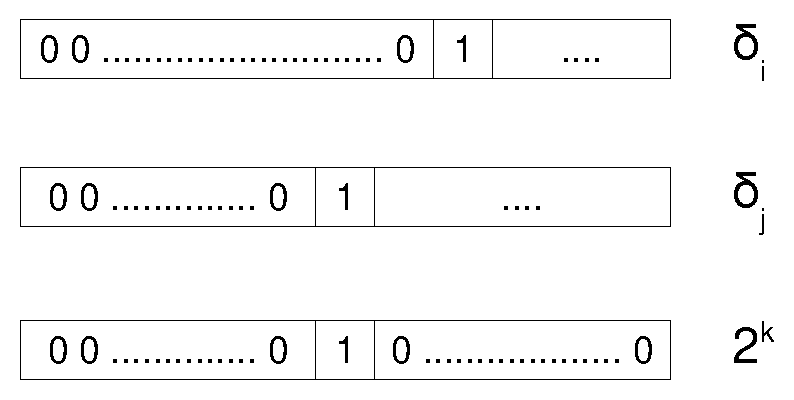
\includegraphics[width=0.4\textwidth]{2.theor/bits}\\
  \caption{Перекрашивание и битовые строки}\label{fig:bits}
\end{figure}

Итак, система ограничений для описания обращений по ключу $k_i$ в регион $R_i$ согласно методу полезных обращений для \PseudoLRU:
\begin{itemize}
\item для hit($k_i, R_i$):
$$
\left\{\begin{array}{l}
(k_i||R_i) \in \{(t_1||r_1), ..., (t_m||r_m), (k_1||R_1), ..., (k_{i-1}||R_{i-1})\}\\
\{(t_1||r_1), ..., (t_m||r_m)\} - \mbox{все разные}\\
\sum\limits_{j=1}^m [u_{k_i,R_i,\pi'_i}(t_j||r_j)] + \sum\limits_{j=1}^{i-1} [u_{k_i,R_i,\pi'_i}(k_j||R_j)] < W\\
\end{array} \right.
$$
\item для miss($k_i, R_i$):
$$
\left\{\begin{array}{l}
(k_i||R_i) \in \{(t_1||r_1), ..., (t_m||r_m), (k_1||R_1), ..., (k_{i-1}||R_{i-1})\}\\
\{(t_1||r_1), ..., (t_m||r_m)\} - \mbox{все разные}\\
\sum\limits_{j=1}^m [u_{k_i,R_i,\pi'_i}(t_j||r_j)] + \sum\limits_{j=1}^{i-1} [u_{k_i,R_i,\pi'_i}(k_j||R_j)] \geqslant W\\
\end{array} \right.
$$
\end{itemize}

$$u_{k_i,R_i,\pi'_i} (s_j)  \equiv \left\{\begin{array}{l}
(k_i||R_i) \notin \{s_j, s_{j+1}, ..., s_{m+n}\}\\
R_i = R(s_j)\\
(\pi'_i||R_i) \in \{(\pi_j||R_j), (\pi_{j+1} || R_{j+1}), ..., (\pi_{m+n}||R_{m+n})\}\\
\bigwedge\limits_{l = j+1}^{m+n} (R_j = R_l ~\wedge~(\pi'_i||R_i) \notin \{(\pi_j||R_j), (\pi_{j+1}||R_{j+1}), ..., (\pi_l||R_l)\}\\
 \hspace{2cm} \rightarrow P(\pi_j \oplus \pi'_i, \pi_l \oplus \pi'_i))\\
\end{array}\right.
$$
$$s \equiv \langle (t_1,r_1), (t_2,r_2), ..., (t_m,r_m), (k_1, R_1), ..., (k_n,R_n) \rangle$$
$$R(s_i) \mbox{~--- вторая компонента~} s_i$$
$$P(x, y) \equiv (y > x~~\wedge~~x \oplus y > x)$$


%Таблица~\ref{plru_table} содержит ограничения для разных случаев
%кэш-попаданий и кэш-промахов (см. утверждение~\ref{hit_miss_human}).
%В каждое из них включается ограничение на количество полезных
%инструкций согласно предлагаемой методике использования функций
%полезности. Полезности считаются относительно некоторого кэш-промаха
%(для их перебора используется сокращение $x_m : \mbox{miss}$).

В приложении~\ref{sec:proofs} доказана теорема~\ref{PLRUusefulThm} эквивалентности этих формул определению стратегии вытеснения \PseudoLRU.

Немного изменив формулу для $\pi'_i$, можно упростить ограничения \textbf{для}\\ \textbf{успешных} обращений. А именно, определив $\pi'_i$ так:

$$
\begin{array}{l}
\texttt{(ite~} (s_i = s_{i-1}) ~~ (\pi'_i = \pi_{i-1})\\
\texttt{(ite~} (s_i = s_{i-2}) ~~ (\pi'_i = \pi_{i-2} \wedge \pi'_i \neq \pi_{i-1})\\
...\\
\texttt{(ite~} (s_i = s_j) ~~ (\pi'_i = \pi_j \wedge \pi'_i \notin \{\pi_{j+1}, ..., \pi_{i-1}\})\\
... \texttt{~true )))...)}\\
\end{array}
$$

для hit($k_i, R_i$) будет достаточно таких ограничений:
$$
\left\{\begin{array}{l}
(k_i||R_i) \in \{(t_1||r_1), ..., (t_m||r_m), (k_1||R_1), ..., (k_{i-1}||R_{i-1})\}\\
\{(t_1||r_1), ..., (t_m||r_m)\} - \mbox{все разные}\\
\end{array} \right.
$$
т.е. ограничение на сумму будет автоматически выполнено. Этот факт следует из того, что о возможности вытеснения можно вести речь там, где встречается хотя бы одно неуспешное обращение на позиции $\pi'_i$. Если же позиция $\pi'_i$ не встречается после последнего обращения к ключу $k_i$, то и вытеснение произведено не будет (в формулах полезных обращений третье условие ложно для всех $s_j$, значит, количество полезных обращений равно равно 0, что означает невытеснение).

\subsection{Разрешение ограничений, описывающих стратегии вытеснения}

Ограничения, которые предлагается строить для описания количества полезных обращений, являются \emph{ограничениями мощности} (cardinality constraints). Это
ограничения вида $C_1 \leqslant \sum_{i=1}^n a_i \leqslant C_2$, где $C_1, C_2$
-- неотрицательные целые числа, а $a_i$ принимают значения 0 или
1~\cite{smt_debugging, PiskacK08, KuncakR07,
Revesz05}. Речь идет об ограничении размера некоторого множества
элементов, заданного с помощью характеристической функции.
В~\cite{smt_debugging} проведено исследование способов записи
ограничений мощности и показано, что от формы записи зависит
эффективность разрешения этих ограничений. Одна из таких форм рассматривает ограничения
мощности как компактную форму записи уравнения
вида $\bigvee_{C_1 \leqslant C \leqslant C_2} \sum_{i=1}^n a_i = C$,
где равенство есть
\begin{itemize}
\item тождественная ложь, если $C < 0$ или $C > n$;
\item конъюнкция $\bigwedge_{1\leqslant i\leqslant n} (a_i = 0)$,
если $C = 0$;
\item дизъюнкция по всевозможным выборкам индексов $i_1, ..., i_C$, где
для каждого индекса $i_k$ справедливы свойства $1 \leqslant i_k
\leqslant n$ и $i_k < i_{k+1}$, конъюнкций $\bigwedge_{i_k} (a_{i_k}
= 1)$, если $1 \leqslant C \leqslant n$.
\end{itemize}

В диссертации не ставилась задача исследования способов разрешения ограничений
мощности (с целью выбора наиболее эффективного способа их представления). Вместо
этого были использованы
имеющиеся инструменты разрешения ограничений мощности~\cite{Z3, Yices}. Для
записи оставшихся формул был использован язык битовых строк, для разрешения
ограничений над которым существуют эффективные SMT-инструменты (например,
Z3~\cite{Z3}).

%После устранения ограничений мощности в формуле остаются только
%ограничения на конечные множества тегсетов: принадлежности и
%непринадлежности тега конечному множеству тегсетов и равенства и
%неравенства битовых полей тегсетов. Поскольку конечные множества
%тегсетов известны (заданы перечислением тегсетов, которые в входят в
%это множество), то ограничения принадлежности и непринадлежности
%могут быть переписаны без использования этих отношений. Отношение
%принадлежности $x \in \{x_1, x_2, ..., x_n\}$ может быть переписано
%в виде дизъюнкции $(x = x_1) \vee (x = x_2) \vee ... \vee (x =
%x_n)$, а отношение непринадлежности $x \notin \{x_1, x_2, ...,
%x_n\}$ -- в виде конъюнкции $(x \neq x_1) \wedge (x \neq x_2) \wedge
%... \wedge (x \neq x_n)$.
%
%В результате получается предикат, в котором переменными величинами
%являются неотрицательные целые числа с конечной областью значений
%(тегсеты), над переменными возможны операции получения битового
%поля, в предикате используется отношение равенства и неравенства над
%битовыми полями. Кроме того, этот предикат задается с использованием
%ограничений мощности.
%
%Для разрешения такого рода предикатов можно было бы разрабатывать
%собственные процедуры распространения ограничений, но это свело бы
%на нет все усилия по выработке собственного представления стратегии
%вытеснения. Однако предлагаемые ограничения могут быть тривиальным
%образом выражены на языке теорий, для которых существуют эффективные
%разрешающие процедуры (битовые строки, неинтерпретируемые функции).
%Поэтому для записи и разрешения этих ограничений могут быть
%использованы SMT-инструменты~\cite{Z3}.

%%%%%%%%%%%%%%%%%%%%%%%%%%%%%%%%%%%%%%%%%%%%%%%%%%%%%%%%%%%%%%%%%%%
%
%\pagebreak
%\section{Ограничения, описывающие тестовые ситуации в некоторых
%частных случаях, для стратегии вытеснения \LRU}
%
%\subsection{Тестовые шаблоны без кэш-промахов}
%
%В случае тестовых шаблонов, в которых нет кэш-промахов, нет ни
%вытесняющих, ни вытесняемых тегсетов. Поэтому в таких шаблонов
%уравнения для кэш-попаданий имеют очень простой вид:
%
%$$
%\left\{
%\begin{array}{l}
%x \in D\\
%... (\mbox{тестовые ситуации на остальные буферы})\\
%\end{array}
%\right.
%$$
%
%\subsection{Тестовые шаблоны без кэш-попаданий}
%
%В случае тестовых шаблонов, в которых нет кэш-попаданий, надо
%генерировать ограничения для вытесняющих и лишь иногда для
%вытесняемых тегсетов. А именно, вытесняемый тегсет требуется лишь в
%том случае, когда кэш-промах вносит в кэширующий буфер ранее
%вытесненный тегсет. В этом случае для вытесняемого тегсета известен
%домен, что позволяет построить уравнения обозримого размера. Кроме
%того, поскольку отсутствуют кэш-попадания, повторные обращения к
%вытесняемым тегсетам (кроме кэш-промаха, который их может внести в
%кэширующий буфер) невозможны, что также упрощает генерируемые
%уравнения.
%
%В результате получается, что вытесняющий тегсет описывается в
%тестовом шаблоне без кэш-попаданий следующей системой уравнений:
%$$
%F'(x) \vee F''(x) \vee \bigvee_{\lambda_\delta \in D} F'''(x, \lambda_\delta)
%$$
%
%где
%
%$$F'(x) \equiv (x \notin D \wedge x \notin \{x_1, ..., x_n\})$$
%
%$$F''(x) \equiv (x \in \{x_1, ..., x_n\} \wedge \sum_{i=1}^n u''(x_i) \geqslant w)$$
%
%$$u''(x_i) \equiv (x\notin \{x_i, ..., x_n\} \wedge R(x_i) = R(x))$$
%
%$$F'''(x, \lambda_\delta) \equiv (x = \lambda_\delta \wedge x \notin
%\{x_1, ..., x_n\} \wedge \sum_{i=1}^n (R(x_i) = R(x)) \geqslant w -
%\delta + 1)$$
%
%\subsection{Короткие тестовые шаблоны}
%
%Будем называть тестовый шаблон \emph{коротким}, если в нем не более
%$w$ инструкций обращения к памяти. Очевидно, что любой короткий
%тестовый шаблон является простым. Из 7 случаев для коротких тестовых
%шаблонов остается всего 5 (первые два можно еще объединить в более
%компактную систему уравнений). В таблице~\ref{short_templates_table}
%предъявлены функции полезности и ограничения для коротких тестовых
%шаблонов в случае стратегии вытеснения \LRU. Соответствующая теорема
%корректности этих ограничений сформулирована и доказана в
% приложении~\ref{sec:proofs}.
%
%\begin{table}[t]
%\begin{tabular}{|c|c|c|c|}
%\hline  & \centering случай &
%\begin{tabular}{c}переменная\\перебора\end{tabular} & система \\
%\hline \hline \multirow{-2}{*}{\rotatebox{90}{кэш-попадание}} &
%\makecell[c{p{0.3\textwidth}}]{тегсет находится в начальном
%состоянии буфера и он всё ещё не вытеснен} & $\lambda_\delta \in D$
%&
%$\left\{\begin{array}{l} x = \lambda_\delta\\
%\sum\limits^n_{i=1} u(x_i) \leqslant w - \delta
%\end{array}\right.$ \\ \hhline{~|---}
%& \makecell[c{p{0.3\textwidth}}]{тегсет уже встречался в шаблоне} &
%-- & $x \in \{x_1, ..., x_n\}$
%\\ \hline \hline \multirow{6}{*}{\rotatebox{90}{кэш-промах}}
%& \makecell[c{p{0.3\textwidth}}]{тегсет встречается впервые} & -- &
%$\left\{\begin{array}{l} x \notin D\\
%x \notin \{x_1, ..., x_n\}\\
%\end{array}\right.$\\ \hhline{~|---} &
%\makecell[c{p{0.3\textwidth}}]{тегсет находился в начальном
%состоянии буфера и был вытеснен} & $\begin{array}{c}\lambda_\delta
%\in D,\\\delta \geqslant w-n+1\end{array}$ &
%$\left\{\begin{array}{l} x = \lambda_\delta\\
%x \notin \{x_1, ..., x_n\}\\
%\sum\limits^n_{i=1} u(x_i) > w - \delta\\
%\end{array}\right.
%$ \\ \hline
%\end{tabular}
%
%%где функция полезности определена следующим образом:
%$$u(x_i) \equiv
%\left\{\begin{array}{l} x_i \in \{ \lambda_{\delta+1}, ...,
%\lambda_w\}~\wedge~x_i \notin \{x_1, ..., x_{i-1}\}, \mbox{если}~S_i
%= \mbox{hit}\\
%R(x_i) = R(x), \mbox{если}~S_i = \mbox{miss}
%\end{array}\right.
%$$
%\caption{Таблица систем уравнений для тестовых ситуаций в кэширующих
%буферах для коротких тестовых шаблонов в случае стратегии вытеснения
%\LRU}\label{short_templates_table}
%\end{table}
%
%
%
%%\begin{landscape}
%%\begin{table}
%%\begin{tabular}{|c|c|c|c|c|c|}
%%\hline  & \centering случай &
%%\begin{tabular}{c}переменная\\перебора\end{tabular} & система &
%%\begin{tabular}{c}функция\\полезности\\для кэш-\\попадания\end{tabular} &
%%\begin{tabular}{c}функция\\полезности\\для кэш-\\промаха\end{tabular} \\
%%\hline \hline \multirow{-2}{*}{\rotatebox{90}{кэш-попадание}} &
%%\makecell[c{p{0.3\textwidth}}]{тегсет находится в начальном
%%состоянии буфера и он всё ещё не вытеснен} & $\lambda_\delta \in
%%D$ &
%%$\left\{\begin{array}{l} x = \lambda_\delta\\
%%\sum\limits^n_{i=1} u(x_i) \leqslant w - \delta
%%\end{array}\right.
%%$ &
%%\begin{tabular}{c}
%%$x_i \in \{ \lambda_{\delta+1}, ..., \lambda_w\}$\\
%%$\wedge~x_i \notin \{x_1, ..., x_{i-1}\}$
%%\end{tabular}
%%& $R(x_i) = R(x)$
%%\\ \hhline{~|-----}
%%& \makecell[c{p{0.3\textwidth}}]{тегсет уже встречался в шаблоне} &
%%-- & $x \in \{x_1, ..., x_n\}$ & -- & --
%%\\ \hline \hline \multirow{6}{*}{\rotatebox{90}{кэш-промах}}
%%& \makecell[c{p{0.3\textwidth}}]{тегсет встречается впервые} & -- &
%%$\left\{\begin{array}{l} x \notin D\\
%%x \notin \{x_1, ..., x_n\}\\
%%\end{array}\right.
%%$ & -- & -- \\ \hhline{~|-----} &
%%\makecell[c{p{0.3\textwidth}}]{тегсет находился в начальном
%%состоянии буфера и был вытеснен} &
%%$\begin{array}{c}\lambda_\delta \in D,\\\delta \geqslant
%%w-n+1\end{array}$ &
%%$\left\{\begin{array}{l} x = \lambda_\delta\\
%%x \notin \{x_1, ..., x_n\}\\
%%\sum\limits^n_{i=1} u(x_i) > w - \delta\\
%%\end{array}\right.
%%$ &
%%\begin{tabular}{c}
%%$x_i \in\{\lambda_{\delta+1}, ..., \lambda_w\}$\\
%%$\wedge~x \notin \{x_1, ..., x_{i-1}\}$\\
%%\end{tabular}
%%&
%%\begin{tabular}{c}
%%$R(x_i) = R(x)$\\
%%\end{tabular}
%%\\ \hline
%%\end{tabular}
%%\caption{Таблица систем уравнений для тестовых ситуаций в кэширующем буфере
%%для коротких тестовых шаблонов в случае стратегии вытеснения
%%\LRU}\label{short_templates_table}
%%\end{table}
%%\end{landscape}
%
%
%\subsection{Генерация тестовых данных для кэш-памяти, содержащей
%<<грязные>> ячейки}
%
%Любая ячейка в кэш-памяти может быть помечена \emph{грязной}
%(\emph{invalid}). Это означает, что данные, находящиеся в кэширующем
%буфере по этому адресу, не могут использоваться в качестве данных,
%хранящихся в памяти по этому адресу.
%
%Рассмотренные ранее в этой работе случаи не учитывали грязные ячейки
%кэширующем буфере, хотя они зачастую присутствуют в микропроцессоре
%после его запуска -- с таким состоянием кэширующего буфера работают
%первые после запуска микропроцессора инструкции.
%
%Кэш-попадание возникает в том случае, когда требуемые данные
%присутствуют среди <<чистых>> ячеек кэширующего буфера. Кэш-промах
%возникает в том случае, когда требуемых данных нет среди <<чистых>>
%ячеек. Причем при наличии <<грязных>> ячеек вытеснения может и не
%произойти. А именно, если все ячейки набора, с которым работает
%инструкция, являются <<чистыми>>, то происходит вытеснение согласно
%стратегии вытеснения, остальные наборы не меняются. Если же среди
%ячеек набор есть <<грязные>> ячейки, то вытеснение не происходит, а
%на место одной из <<грязных>> ячеек помещаются данные из основной
%памяти по заданному адресу и ячейка объявляется <<чистой>>.
%Остальные ячейки не меняются. В стратегии вытеснения \LRU эта бывшая
%<<грязная>> ячейка становится самой новой.
%
%Для генерации тестовых данных для кэширующих буферов с грязными
%ячейками предлагается применять ограничения с функциями полезности.
%Примечательно, что наличие грязных ячеек не меняет качественно
%систему уравнений.
%
%В данном разделе рассматривается случай, когда начальное состояние
%микропроцессора известно. Кроме того, рассматриваемый случай
%учитывает отсутствие инструкций в тестовом шаблоне, которые
%превращали бы <<чистые>> ячейки в <<грязные>> (т.е. все такие
%изменения должны делаться явно вне тестовых шаблонов).
%
%\subsubsection{случай полностью-ассоциативного кэширующего буфера}
%
%В случае полностью-ассоциативных кэширующих буферов очевидно, что
%первые кэш-промахи будут заполнять <<грязные>> ячейки. Пусть $N$ --
%количество <<грязных>> ячеек в начальном состоянии кэширующего
%буфера, а $L_0$ -- начальное состояние (выражение) кэширующего
%буфера (только <<чистые>> ячейки). Тогда для тестовых ситуаций надо
%генерировать такие ограничения ($L$ -- выражение для состояния
%кэширующего буфера перед исполнением инструкции, $L'$ -- выражение
%для состояния кэширующего буфера после исполнения инструкции):
%\begin{itemize}
%\item для \emph{кэш-попадания} hit($x$) генерируются ограничения
%$$
%\left\{
%\begin{array}{l}
%x \in L\\
%L' \equiv L\\
%\end{array}
%\right.
%$$
%
%\item для \emph{кэш-промаха} miss($x$), если это один из первых $N$
%кэш-промахов, генерируются ограничения:
%$$
%\left\{
%\begin{array}{l}
%x \notin L\\
%L' \equiv L \cup \{x\}\\
%\end{array}
%\right.
%$$
%
%\item для \emph{кэш-промаха} miss($x$), являющегося по счету более
%чем $N$'м кэш-промахом тестового шаблона, генерируются ограничения:
%$$
%\left\{
%\begin{array}{l}
%x \notin L\\
%x' \in L\\
%L' \equiv L\setminus\{x'\} \cup \{x\}\\
%displaced(x', L)\\
%\end{array}
%\right.
%$$
%\end{itemize}
%
%Предикат $displaced(x', L)$ истинен, если $x'$ является вытесняемым
%тегом в текущем состоянии кэширующего буфера $L$. Для стратегии
%вытеснения \LRU этот предикат может быть записан с использованием
%тех же диапазонов вытеснения, что и для кэширующего буфера без
%<<грязных>> ячеек (см.п.~\ref{LRU_constraints}). А именно, диапазон
%вытеснения начинается на инструкции, которая последний раз перед
%вытеснением тега обращается к нему. Тогда между этой инструкцией и
%инструкцией, вытесняющей $x$, должны быть обращения ко всем
%остальным тегам текущего состояния кэширующего буфера. Эта логика
%может быть записана в виде тех же уравнений, что и в
%пункте~\ref{LRU_constraints}. Нетрудно проверить, что для
%кэширующего буфера с <<грязными>> ячейками остается справедливой
%лемма о невложенных диапазонах вытеснения, что доказывает
%корректность использования ограничений из
%пункта~\ref{LRU_constraints} для кэширующего буфера с <<грязными>>
%ячейками.
%
%\subsubsection{случай наборно-ассоциативного кэширующего буфера}
%
%В этом пункте будет показано, что ограничения для кэширующего
%буфера, начальное состояние которого содержит <<грязные>> ячейки,
%качественно не отличаются от ограничений для кэширующего буфера без
%<<грязных>> ячеек.
%
%Аналогично тому, как это делалось для кэширующих буферов без
%<<грязных>> ячеек, для тестовых ситуаций на кэширующие буферы с
%<<грязными>> ячейками тоже возможно следующее исчерпывающее
%выделение случаев:
%\begin{itemize}
%\item кэш-попадание тега:
%    \begin{enumerate}
%    \item данный тег находился в начальном состоянии кэширующего буфера и не был
%    вытеснен к моменту данной инструкции;
%    \item данный тег был внесен в кэширующий буфер одной из инструкций
%    кэш-промаха и с тех пор не был вытеснен;
%    \end{enumerate}
%\item кэш-промах тега:
%    \begin{enumerate}
%    \item данный тег не встречался ранее (не находился в начальном
%    состоянии кэширующего буфера и не был внесен какими-либо кэш-промахами);
%    \item данный тег был ранее вытеснен из кэширующего буфера и с тех пор
%    не был внесен в кэширующий буфер вновь.
%    \end{enumerate}
%\end{itemize}
%
%Соответствующие ограничения приведены в
%таблице~\ref{dirty_hit_miss_table}.
%
%
%В таблице~\ref{dirty_hit_miss_table} символ $\Delta$ означает
%количество <<чистых>> ячеек в начальном состоянии того региона, про
%который идет речь в уравнении. На самом деле $\Delta$ есть функция
%региона ($\Delta = \Delta(\lambda_\delta)$), но для сокращения
%записи оставлен только функциональный символ. Кроме того, в
%приведенных уравнениях домен переменной включает только <<чистые>>
%ячейки.
%
%Сходства уравнений (со случаем кэширующих буферов без <<грязных>>
%ячеек) удалось добиться за счет рассмотрения <<грязных>> ячеек, как
%ячеек с наименьшим счетчиком \LRU, которые не участвуют в
%определении нахождения тега в кэширующих буферах. Поэтому в функциях
%полезности участвуют множества не $\{\lambda_{\delta+1}, ...,
%\lambda_w\}$, а множества $\{\lambda_{\delta+1}, ...,
%\lambda_\Delta\}$. Все <<чистые>> ячейки получили первые индексы,
%т.е. индексы всех от 1 до $\Delta$.
%
%%\begin{theorem}[корректность использования функций полезности для
%%записи \LRU в случае наличия <<грязных>> ячеек в начальном состоянии
%%кэширующего буфера] Тестовая программа, построенная по ограничениям,
%%которые сгенерированы с использованием предъявленных в
%%таблице~\ref{dirty_hit_miss_table} функций полезности, в случае
%%наличия <<грязных>> ячеек в начальном состоянии кэширующего буфера
%%удовлетворяет своему тестовому шаблону.
%%\end{theorem}
%%\begin{proof}
%%  //TODO
%%\end{proof}
%
%Для приведенных ограничений также могут быть применены эвристики,
%сокращающие их количество, которые были упомянуты для кэширующих
%буферов без <<грязных>> ячеек. Кроме того, в данном случае возможна
%дополнительная эвристика \emph{ограничение на $\delta$}: если
%$\delta + 1 < \Delta$, то функция полезности, в которую входит
%множество $\{\lambda_{\delta+1}, ..., \lambda_\Delta\}$, равна 0.
%
%%\subsection{Функции полезности для зеркальной генерации тестовых
%%данных}
%%
%%Рассмотрим ограничения, генерируемые для тестовых шаблонов
%%зеркальным методом с использованием функций полезности. По сравнению
%%с представленными ограничениями (см. табл.~\ref{hit_miss_table})
%%зеркальная генерация имеет свои особенности:
%%\begin{enumerate}
%%  \item множества констант (как, например, $L, D$) не используются,
%%  поэтому в ограничениях будут отсутствовать соответствующие им
%%  случаи;
%%  \item так как теги инструкций тестового шаблона должны появиться
%%  среди инициализирующей последовательности, то для вытеснения
%%  требуется $w-1$ инструкций, где $w$ -- ассоциативность кэширующего буфера;
%%  \item учет полезных инструкций начинается уже в инициализирующей
%%  последовательности, тем самым необходимо сформулировать функцию
%%  полезности для инициализирующих инструкций.
%%\end{enumerate}
%%
%%Следующая теорема описывает функцию полезности для инициализирующих
%%инструкций и описывает ограничения, генерируемые для тестовых
%%шаблонов зеркальным методом с использованием функций полезности
%%(количество инициализирующих инструкций зафиксировано, оно будет
%%обозначено параметром $m$):
%%
%%\begin{theorem}[Корректность ограничений, генерируемые зеркальным методом с
%%использованием функций полезности для
%%\LRU]\label{correct_mirror_LRU} Пусть $t_1, t_2, ..., t_m$ -- теги
%%инициализирующей последовательности, $x$ -- текущий тег тестового
%%шаблона, $x_1, x_2, ..., x_n$ -- теги предыдущих инструкций
%%тестового шаблона, причем $x \in \{t_1, ..., t_m, x_1, ..., x_n\}$ и
%%$\{t_1, ..., t_m\}$ --- все разные. Тогда $x$ не вытеснен согласно
%%определению на списках тогда и только тогда, когда
%%$$\sum\limits_{i=1}^{m+n} u_x(s_i) < w$$
%%где последовательность $s \equiv \langle t_1, ..., t_m, x_1, ...,
%%x_n\rangle$, а функция полезности определена следующим образом:
%%$$u_x(s_i) \equiv (x \notin \{s_i, ..., s_{m+n}\} \wedge
%%R(x) = R(s_i) \wedge s_i \notin\{s_{i+1},..., s_{m+n}\})$$
%%
%%%$$\sum\limits_{i=1}^m \tilde{u}_x(t_i) + \sum\limits_{i=1}^n u_x(x_i) < w$$
%%%где функции полезности определены следующим образом:
%%%$$\begin{array}{c}
%%%\tilde{u}_x(t_i) \equiv (x \notin \{t_i, ..., t_m, x_1, ..., x_n\}
%%%\wedge R(x) = R(t_i))\\u_x(x_i) \equiv (x \notin \{x_i, ..., x_n\}
%%%\wedge R(x) = R(x_i))\end{array}$$
%%
%%%$$\begin{array}{c}u_x(x_i) \equiv (x \notin \{x_i, ..., x_n\} \wedge R(x) =
%%%R(x_i)), \mbox{если}~S_i=\mbox{miss}\end{array}$$
%%%$$\begin{array}{c}u_x(x_i) \equiv (x \notin \{x_i, ..., x_n\} \wedge R(x) =
%%%R(x_i) \wedge \sum\limits_{j=1}^{m} \tilde{c}_{x_i}(t_j) = 0
%%%\wedge \sum\limits_{j=1}^{i-1} c_i(x_j) = 0),\\
%%%\mbox{если}~S_i=\mbox{hit}\end{array}$$
%%%$$c_i(x_j) \equiv (x \notin \{x_j, ..., x_{i-1}\} \wedge x_i = x_j)$$
%%%$$\tilde{c}_{x_i}(t_j) \equiv (x \notin \{t_j, ..., t_m, x_1, ..., x_{i-1}\} \wedge x_i = t_j)$$
%%\end{theorem}
%%\begin{proof}
%%//TODO написать правильное доказательство
%%
%%сумма полезных - это количество различных тегов, тогда полезными будем считать
% инструкции тестового шаблона, которые обращаются к разным тегам, при этом ко
% всем различным тегам есть инструкция; различные - например, последние; отсюда и
% функция полезности.
%%
%%%Воспользуемся леммой~\ref{hit_II}. При этом в качестве
%%%последовательности тегов тестового шаблона в этой лемме рассмотрим
%%%последовательность $t_1, t_2,~\dots,~t_m,~x_1,~x_2,~\dots,~x_n$.
%%%Согласно лемме тестовая ситуация на $x$ выполнена при
%%%соответствующем условии на сумму функций полезности от элементов
%%%этой последовательности. Функции полезности для
%%%$x_1,~x_2,~\dots,~x_n$ без изменений переходят из формулировки
%%%леммы~\ref{hit_II} в данную теорему. Функцию полезности для $t_1,
%%%t_2,~\dots,~t_m$ из формулировки леммы~\ref{hit_II} получить нельзя,
%%%поскольку неизвестна тестовая ситуация на эти теги. Однако, вспомнив
%%%определение полезной инструкции, функцию полезности для этих тегов
%%%получить несложно. А именно, тег $t_i$ будет полезным, если он
%%%продвигает $x$ к концу списка \LRU после последнего обращения к $x$.
%%%Если после последнего обращения к $x$ сам тег $t_i$ встречается
%%%впервые, то он будет полезным (см. доказательство
%%%леммы~\ref{hit_II}). Если же после последнего обращения к $x$ $t_i$
%%%встречается не в первый раз, то он не двигает $x$ к концу списка,
%%%что, тем самым, означает бесполезность $t_i$. Но поскольку все $t_i$
%%%разные, то повторное обращение возможно лишь среди
%%%$x_1,~x_2,~\dots,~x_n$ -- поэтому в функцию полезности для этих
%%%тегов добавлено отличие от $t_1,~t_2,~\dots,~t_m$.
%%\end{proof}
%%%\begin{sld}[Корректность ограничений, генерируемые зеркальным методом с
%%%использованием функций полезности для полностью ассоциативного \LRU
%%%буфера] Пусть $t_1, t_2, ..., t_m$ -- теги инициализирующей
%%%последовательности, $x$ -- текущий тег тестового шаблона, $x_1, x_2,
%%%..., x_n$ -- теги предыдущих инструкций тестового шаблона, причем $x
%%%\in \{t_1, ..., t_m, x_1, ..., x_n\}$ и $\{t_1, ..., t_m\}$ --- все
%%%разные. Тогда $x$ не вытеснен из полностью ассоциативного буфера
%%%согласно определению на списках тогда и только тогда, когда
%%%$$x \in \{s_{m+n-w+1}, ..., s_{m+n}\}$$ где последовательность $s
%%%\equiv \langle t_1, ..., t_m, x_1, ..., x_n\rangle$.
%%%\end{sld}
%%%\begin{proof}
%%%  //TODO
%%%\end{proof}
%%
%%Из теоремы~\ref{correct_mirror_LRU} следует система уравнений для
%%описания тестовой ситуации $S$ тега $x$, генерируемая зеркальным
%%методом с использованием функций полезности для \LRU (функции
%%полезности приведены в формулировке
%%теоремы~\ref{correct_mirror_LRU}):
%%\begin{itemize}
%%\item если $S$ = hit, то
%%$$
%%\left\{\begin{array}{l} x \in \{t_1, ..., t_m, x_1, ..., x_n\}\\
%%\sum\limits_{i=1}^m u_x(t_i) + \sum\limits_{i=1}^n u_x(x_i) < w\\
%%\{t_1, ..., t_m\} - \mbox{все разные}\\
%%\end{array} \right.
%%$$
%%\item если $S$ = miss, то
%%$$
%%\left\{\begin{array}{l} x \in \{t_1, ..., t_m, x_1, ..., x_n\}\\
%%\sum\limits_{i=1}^m u_x(t_i) + \sum\limits_{i=1}^n u_x(x_i)
%%\geqslant w\\
%%\{t_1, ..., t_m\} - \mbox{все разные}\\
%%\end{array} \right.
%%$$
%%\end{itemize}
%%
%%%Стоит заметить, что функции полезности добавили новое дополнительное
%%%условие на теги инициализирующих инструкций: они должны быть
%%%различными. В этом выражается свойство <<простоты>> инициализирующей
%%%последовательности, эта последовательность не должна содержать
%%%сложной внутренней последовательности изменений состояния
%%%кэширующего буфера.


\section{Конструирование тестовой программы для кэш-памяти первого и второго
уровня}\label{sec:L1L2_initialization}

В результате разрешения ограничений для каждой таблицы будет сгенерирована инициализирующая последовательность ключей, регионов и данных. Как уже было сказано, задачей
конструктора тестовых программ является построение инструкций микропроцессора,
которые осуществляют вычисленные обращения. Для написания конструктора тестовых
программ надо выяснить из документации по архитектуре способы исполнения
инструкций, при которых задействованы различные таблицы. Если для таблицы
нашлась инструкция, которая может произвести в нее обращение независимо от
других таблиц (это наиболее частый случай), то эту инструкцию и рекомендуется использовать в конструкторе. Более сложный
случай --- если такой инструкции найти не удается. В данном разделе будет
показан один такой случай и возможное поведение конструктора тестовой программы
для него.

Речь идет о кэш-памяти первого и второго уровня. Если обращение в кэш-память
первого уровня оказывается успешным, то обращение в кэш-память
второго уровня не производится. Получается, что последовательность обращений в
кэш-память второго уровня влияет на последовательность обращений в кэш-память
первого уровня: чтобы произошло обращение в кэш-память второго уровня, обращение
в кэш-память первого уровня должно быть неуспешным; и, наоборот, при неуспешном
обращении в кэш-память первого уровня возможно обращение в кэш-память второго
уровня (которое может нарушить построенную инициализирующую последовательность
для нее), правда, обращение к кэш-память второго уровня некоторые
микропроцессоры позволяют запретить (например, микропроцессоры
MIPS~\cite{mips64III}). Но и это еще не всё: обращения в кэш-память обоих
уровней осуществляются по одному и тому же адресу, тем самым для обращения в
кэш-память второго уровня нужен промах обращения по специальному ключу в
кэш-памяти первого уровня.

Поскольку инициализирующие последовательности ключей строятся в предположении
произвольности состояния таблицы перед её выполнением и поскольку обращение в
кэш-память второго уровня обязательно включает в себя обращение в кэш-память
первого уровня, то в тестовой прогармме сначала надо инициализировать кэш-память
второго уровня, а затем уже кэш-память первого уровня. Теперь надо понять, какую
последовательность инструкций надо конструировать для инициализации каждого
уровня кэш-памяти.

Еще раз вспомним, на основе чего надо проводить конструирование: каждый элемент
инициализирующей последовательности --- это ключ, регион и, если необходимо, данные.
Конструируются обычные инструкции, обычная программа на языке ассемблера. Но она
должна осуществлять заданную последовательность обращений, в том числе, в
кэш-память второго уровня. У каждой инструкции есть аргументы. Сконструировать
программу --- значит выбрать последовательность названий инструкций, их аргументы и значения
для аргументов. Ключ и регион -- есть атрибуты адреса (физического или
виртуального), который вычисляется по аргументам инструкции. Значит, ключ и
регион нам даны, по ним надо собрать адрес, по адресу вычислить аргументы и,
наконец, составить инструкцию из них.

\begin{figure}[h] \centering
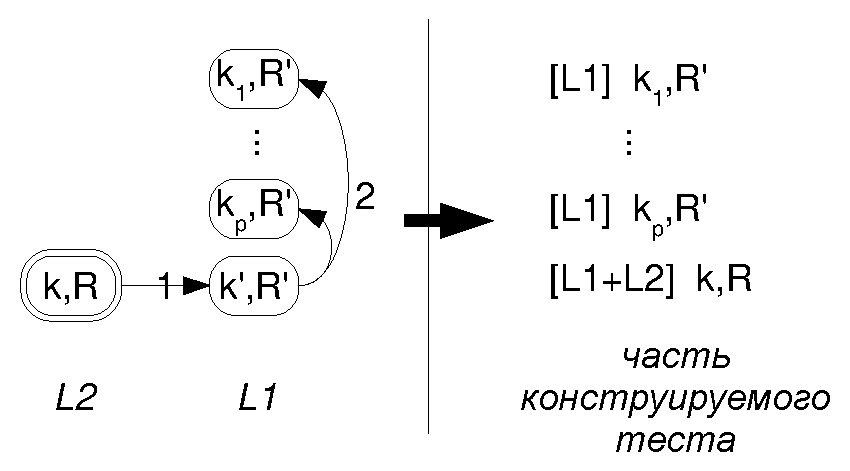
\includegraphics[width=0.6\textwidth]{2.theor/L1L2}
\caption{Конструирование обращения в кэш-память второго уровня вместе с
обращениями в кэш-память первого уровня}\label{fig:L1L2}
\end{figure}

Итак, по ключу и региону для кэш-памяти первого уровня
инструкция составляется по только что приведенной схеме. С одним лишь
уточнением, что адрес в этой инструкции должен быть таким, что при обращении по нему кэш-память
второго уровня не задействована. Теперь разберемся с последовательностью ключей
и регионов для кэш-памяти второго уровня. Рисунок~\ref{fig:L1L2} схематически
показывает, какие дополнительные инструкции надо построить для произвольного
обращения по ключу $k$ в регион $R$ кэш-памяти второго уровня. А именно, ключу
$k$ в регионе $R$ соответствует некоторый адрес, этому же адресу соответствуют и
некоторый ключ $k'$ в регионе $R'$ кэш-памяти первого уровня (стрелка с цифрой
1). Но надо еще обеспечить отсутствие этого ключа, иначе обращения в кэш-память
второго уровня не будет. Для этого надо сгенерировать небольшую
последовательность произвольных различных и не равных $k'$ ключей $k_1, k_2,
\dots, k_p$ и обратиться по ним в регион $R'$ кэш-памяти первого уровня без
затрагивания кэш-памяти второго уровня (значение числа $p$ зависит от стратегии
вытеснения).

%Рассмотрим один часто встречающийся случай кэширующих буферов,
%инициализация которого может вызывать трудности. Речь идет о
%кэш-памяти второго уровня. Зачастую кэш-память второго уровня не
%может быть инициализирована отдельно от остальных подсистем
%микропроцессора, обычно оно связано с изменением кэш-памяти первого
%уровня. Это создает дополнительные сложности при формулировании
%ограничений методом зеркальной генерации, поскольку инициализирующая
%последовательность должна подготавливать сразу два кэширующих буфера
%одновременно -- кэш-память первого уровня и кэш-память второго
%уровня. Кроме того, зачастую кэш-память второго уровня является
%совместной для хранения в ней данных и инструкций. Поэтому на
%инициализацию кэш-памяти второго уровня влияют и сами
%инициализирующие инструкции, и даже адрес расположения тестовой
%программы в памяти (от него зависит виртуальный адрес инструкций, а
%значит теги и индексы при обращении к кэш-памяти инструкций).
%
%Если принять дополнительное требование (и оно даст решение), что в
%кэш-памяти второго уровня наборы, используемые для доступа к
%инструкциям, не пересекаются с наборами, используемыми для доступа к
%данным, то генерируемые ограничения упрощаются (кэширование
%инструкций можно вообще не учитывать). С точки зрения зеркальной
%генерации это означает, что надо сформулировать требования на
%инициализирующую последовательность. Напомню, что одним из ключевых
%требований является произвольность начального состояния
%(содержимого) кэш-памяти.
%
%Предположим, что обращение к кэш-памяти второго уровня
%осуществляется при кэш-промахе в кэш-памяти первого уровня и
%кэш-память не является virtually indexed virtually
%tagged~\cite{HennessyPatterson3rd}. Для составления ограничений с
%использованием функций полезности необходимо знать, которые
%инструкции среди инициализирующей последовательности действительно
%обращаются в кэш-память второго уровня (иными словами, в каких
%инструкциях среди инициализирующей последовательности происходит
%кэш-промах при обращении к кэш-памяти первого уровня). Возможным
%решением было бы перебирать всевозможные распределения тестовых
%ситуаций в кэш-памяти первого уровня на элементах инициализирующей
%последовательности (с предварительной подготовкой этих тестовых
%ситуаций). Однако следующая лемма~\ref{special_initialization_L2}
%показывает, что для любого такого произвольного распределения
%тестовых ситуаций в кэш-памяти первого уровня существует решение со
%специальным распределением тестовых ситуаций. Это позволяет
%перебирать только такие специальные распределения тестовых ситуаций
%в кэш-памяти первого уровня. При этом вычислительная сложность
%процедуры поиска инициализирующей последовательности, дающей
%решение, изменяется от экспоненциальной от длины тестового шаблона к
%полиномиальной, что показывает лемма~\ref{max_k_h} (ее доказательство
%приведено в приложении~\ref{proofs}):
%\begin{lemma}[Верхняя оценка длины специальной инициализирующей
%последовательности для стратегии вытеснения \LRU]\label{max_k_h}\MaxUpperBoundLRU
%\end{lemma}
%\begin{sld}
%$$m = O(n)$$ где $m$ --- длина специальной инициализирующей
%последовательности, $n$ -- количество инструкций тестового шаблона.
%\end{sld}
%
%Для получения инициализирующей программы минимальной длины, можно
%применять сначала двоичный поиск суммы $k+h$ с применением
%дальнейшего поиска допустимых значений $k$ и $h$. 

% !Mode:: "TeX:UTF-8"
\chapter{Применение предлагаемых методов, сравнение с аналогами}

В этой главе показывается, что предлагаемых в диссертации средств моделирования микропроцессоров достаточно для генерации тестовых программ, нацеленных на подсистемы управления памяти, таких трех часто используемых архитектур как MIPS~\cite{mips64II}, PowerPC~\cite{PowerPC} и IA-32~\cite{IA32}. При рассмотрении архитектур важными будут следующие вопросы:
\begin{enumerate}
    \item описываются ли варианты исполнения инструкций в виде ограничений на битовые строки в документации (тогда трудоемкость моделирования вариантов исполнения инструкций была бы ниже);
    \item возможно ли моделирование устройств подсистемы управления памяти; существуют ли устройства, не моделируемые в виде таблиц;
    \item хватает ли предлагаемых в диссертации средств для описания трансляции адресов.
\end{enumerate}

В разделе~\ref{sec:templates_estimation} описаны эксперименты по оценке длины шаблонов, для
которых удается эффективно строить тесты предлагаемыми в диссертации
методами. Заканчивается глава
сравнением особенностей предлагаемого метода генерации тестовых программ по
тестовым шаблонам с методом, предлагаемым инструментом
Genesys-Pro~\cite{GenesysPro}, а также сравнение с некоторыми работами в Intel~\cite{MicroFORMAL}.

%% отвечаем на следующие вопросы:
% 1. описываются ли инструкции в виде ограничений на битовые строки в документации
% 2. описывается ли модель состояния MMU в виде лишь таблиц? нет ли там
% чего-нибудь, не сводящегося к таблице?
% -> структура TLB
% 3. хватает ли средств для описания трансляции адреса ?
% -> поток данных, описывающих трансляцию
% режимы работы (real mode, protected mode)

% таблица - то, что представляется множеством строк,
% строка представляется набором полей ключа и полей данных

%% схема описания компонента MMU:
% 1. поля строк
% 2. количество строк
% 3. битовая длина номера региона (тип таблицы - полностью-ассоциативная, ....)
% 4. стратегия вытеснения
% 5. предикат keyMatch
% 6. особенности компонента (чего-то более одного, чего-то быть не может, ...) -
% например, одна строка хранит несколько подряд данных

% в MIPS R12000 появилась кэш-память адресов переходов (32 строки), но она не
% относится к MMU данных

\section{Генерация тестов для архитектуры MIPS}\label{sec:mips_application}

%\begin{utv}
%Для архитектуры MIPS возможно применение применение методов, описанных в
% диссертации, для генерации тестовых программ по тестовым шаблонам; причем
% методов достаточно
% для полного описания поведения MMU микропроцессоров архитектуры MIPS.
%\end{utv}

Документация по архитектуре MIPS представлена в MIPS64™ Architecture For Programmers (в трех томах)~\cite{mips64II, mips64III}. Второй том (The MIPS64™ Instruction Set) содержит описания инструкций. Они  действительно описываются в виде набора операций над битовыми строками на специальном псевдокоде.% (см.рис.~\ref{fig:mips64_page}).

%\begin{figure}
%\framebox[0.93\textwidth][l]{\parbox{0.9\textwidth}{
%
%\textbf{Load Doubleword    LD}\\
%
%\textbf{Format:} LD rt, offset(base)\\
%
%\textbf{Purpose:} To load a doubleword from memory\\
%
%\textbf{Description:} rt <- memory[base+offset]
%
%The contents of the 64-bit doubleword at the memory location specified by the aligned effective address are fetched and placed in GPR rt. The 16-bit signed offset is added to the contents of GPR base to form the effective address.\\
%
%\textbf{Restrictions:}\\
%The effective address must be naturally-aligned. If any of the 3 least-significant bits of the address is non-zero, an Address Error exception occurs.\\
%
%\textbf{Operation:}
%
%\texttt{vAddr <- sign\_extend(offset) + GPR[base]}
%
%\texttt{if vAddr$_{2..0} \neq 0^3$ then}
%
%\hspace{2cm}\texttt{SignalException(AddressError)}
%
%\texttt{endif}
%
%\texttt{(pAddr, CCA) <- AddressTranslation (vAddr, DATA, LOAD)}
%
%\texttt{memdoubleword <- LoadMemory (CCA, DOUBLEWORD, pAddr, vAddr, DATA)}
%
%\texttt{GPR[rt] <- memdoubleword}\\
%
%\textbf{Exceptions:}\\
%TLB Refill, TLB Invalid, Bus Error, Address Error, Reserved Instruction, Watch
%
%}
%}
%\caption{Пример страницы документации по системе команд архитектуры MIPS64}\label{fig:mips64_page}
%\end{figure}

Третий том (The MIPS64™ Privileged Resource Architecture) содержит описание подсистемы управления памяти в
микропроцессорах MIPS. Для работы с данными она содержит следующие устройства (количественные
характеристики приведены для микропроцессора MIPS R10000~\cite{R10000}):
\begin{itemize}
  \item \emph{кэш-память данных первого уровня (D-Cache-1)}:
        \begin{itemize}
            \item размер: 32 кБ;
            \item поля строк: тэг физического адреса (ключ), данные (данные);
            \item битовая длина номера региона: 6 (наборно-ассоциативная\\ кэш-память);
            \item количество строк в регионе: 2;
            \item стратегия вытеснения \LRU;
        \end{itemize}
  \item \emph{кэш-память второго уровня (Cache-2)}:
        \begin{itemize}
            \item размер: от 512 кБ до 16 МБ;
            \item поля строк: тэг физического адреса для кэш-памяти второго
уровня (ключ), данные (данные) (16 или 32 слова);
            \item количество строк в регионе: 2;
            \item стратегия вытеснения \LRU;
        \end{itemize}
         Cache-2 является внешней;
  \item \emph{TLB (Joint-TLB)}:
        \begin{itemize}
            \item поля строк: r, vpn/2, g, asid (ключи), pfn0, cca0, v0, c0, d0,
pfn1, cca1, v1, c1, d1 (данные);
            \item битовая длина номера региона: 0 (полностью-ассоциативный TLB);
            \item количество строк в регионе: 64;
            \item вытеснение программное (т.е. стратегия вытеснения none);
            \item размер виртуального адреса: 44 бита;
            \item размер физического адреса: 40 бит;
        \end{itemize}
        одна строка TLB хранит информацию про две соседние страницы виртуальной
        памяти;
  \item \emph{буфер TLB (D-TLB)}:
        \begin{itemize}
            \item поля строк те же, что и для Joint-TLB;
            \item битовая длина номера региона: 0 (полностью-ассоциативный);
            \item количество строк в регионе: 8;
            \item стратегия вытеснения \LRU;
        \end{itemize}
\end{itemize}

Другие устройства для обращения в память не используются.

Осталось показать, что трансляция адреса также может быть представлена в виде отношений на битовых строках и обращений к таблицам. Обычное выполнение обращения в память в MIPS следующее:
\begin{enumerate}
    \item на основе аргументов инструкции формируется \emph{виртуальный адрес} (VA);
    \item заменой в виртуальном адресе номера страницы виртуальной памяти на номер фрейма физической памяти формируется \emph{физический адрес} (PA);
    \item по физическому адресу, если нужно, осуществляется обращение в кэш-память или обращение в оперативную память.
\end{enumerate}

\begin{figure}[h] \center
  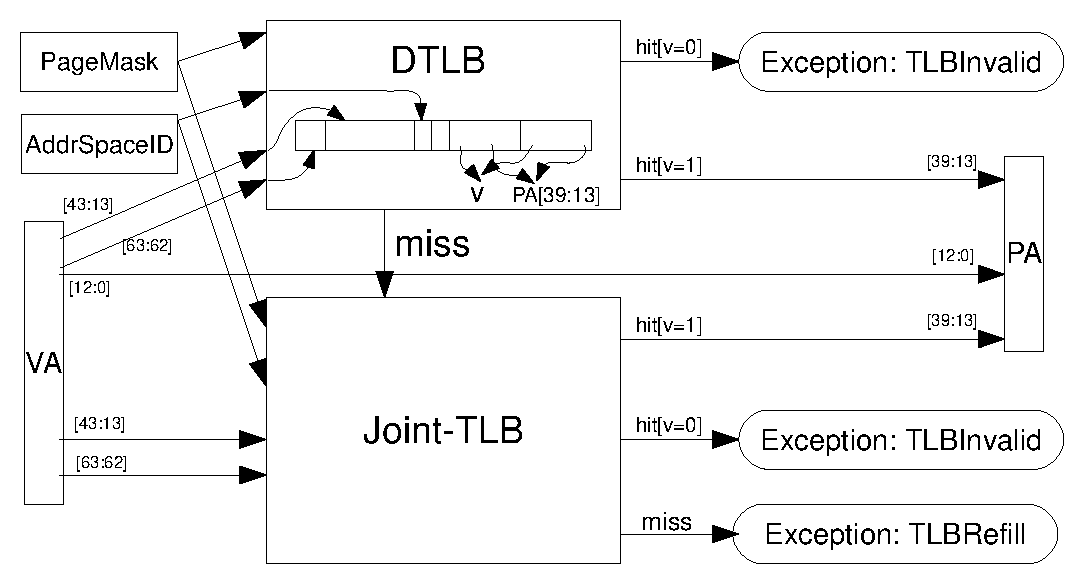
\includegraphics[width=0.8\textwidth]{4.analysis/mips_addrtrans}\\
  \caption{Трансляция адреса в MIPS}\label{fig:mips_address_translation}
\end{figure}


В зависимости от значения виртуального адреса и состояния управляющих регистров
возможны следующие варианты трансляции адреса:
\begin{itemize}
  \item для виртуального адреса трансляция проходит через TLB
(см.рис.~\ref{fig:mips_address_translation});
  \item для виртуального адреса трансляция проходит без таблиц (физический адрес
--- битовая строка --- является результатом битовых операций над виртуальным
адресом --- битовой строкой).
\end{itemize}

%Пример модели инструкции LD с рисунка~\ref{fig:mips64_page} приведен в приложении~\ref{sec:xml}.

\section{Генерация тестов для архитектуры PowerPC}\label{sec:ppc_application}

Архитектура PowerPC разработана компанией IBM. Документация по архитектуре
PowerPC представлена в PowerPC Architecture Book (в трех томах)~\cite{PowerPC}. Первый том (PowerPC User Instruction Set Architecture) содержит описания инструкций. Они действительно описываются в виде набора операций над битовыми строками на специальном псевдокоде (см.рис.~\ref{fig:ppc_page}.

\begin{figure}
\framebox[0.93\textwidth][l]{\parbox{0.9\textwidth}{
\textbf{Store Halfword Indexed X-form}

sthx RS,RA,RB\\


\texttt{if RA = 0 then b <- 0}

\texttt{else \hspace{2cm}  b <- (RA)}

\texttt{EA <- b + (RB)}

\texttt{MEM(EA, 2) <- (RS)$_{48:63}$}\\

Let the effective address \texttt{(EA)} be\\ the sum \texttt{(RA|0)+(RB)}. \texttt{(RS)$_{48:63}$} \\are stored into the halfword in storage\\ addressed by \texttt{EA}.\\

\textbf{Special Registers Altered:}\\
None
}}
\caption{Пример страницы документации системы команд PowerPC}\label{fig:ppc_page}
\end{figure}

Третий том (PowerPC Operating Environment Architecture) содержит описание подсистемы управления памяти в микропроцессорах PowerPC. Для работы с данными она содержит следующие устройства (количественные характеристики приведены для микропроцессора PowerPC 970FX
~\cite{PowerPC970FXUserManual}):
\begin{itemize}
  \item \emph{кэш-память данных первого уровня (D-Cache-1)}:
        \begin{itemize}
            \item размер: 32 кБ;
            \item поля строк: тэг физического адреса (ключ), данные (данные);
            \item битовая длина номера региона: 7 (наборно-ассоциативная\\кэш-память);
            \item количество строк в регионе: 2;
            \item стратегия вытеснения \LRU;
        \end{itemize}
  \item \emph{кэш-память второго уровня (Cache-2)}:
        \begin{itemize}
            \item размер: 512 кБ;
            \item поля строк: тэг физического адреса (ключ), данные (данные);
            \item битовая длина номера региона: 11 (наборно-ассоциативная кэш~--~память);
            \item количество строк в регионе: 8;
            \item стратегия вытеснения \LRU;
        \end{itemize}
  \item \emph{D-TLB} (кэш таблицы страниц):
        \begin{itemize}
            \item поля строк: номер страницы виртуальной памяти (ключ), номер\\фрейма физической памяти (данные);
            \item битовая длина номера региона: 8 (наборно-ассоциативный);
            \item количество строк в регионе: 4;
            \item стратегия вытеснения \LRU;
        \end{itemize}
  \item \emph{сегментные регистры (SLB, Segment Lookaside Buffer)}:
        \begin{itemize}
            \item поля строк: effective segment id (ключ), virtual segment id
(данные), биты K$_s$/K$_p$, V, N, L, C (данные);
            \item битовая длина номера региона: 0 (полностью ассоциативный);
            \item количество строк в регионе: 64;
            \item вытеснение программное;
        \end{itemize}
        используются для получения виртуального адреса по эффективному;
%  \item \emph{буфер непосредственной трансляции адресов (D-ERAT)}:
% НЕТ ЭТОГО БУФЕРА В АРХИТЕКТУРЕ!!! его добавили в самом микропроцессоре
% PPC970FX
%        \begin{itemize}
%            \item поля строк: номер <<эффективной страницы>> (ключ), номер
% фрейма физической памяти (данные), биты (данные);
%            \item битовая длина номера региона: 6 (наборно-ассоциативная
% таблица);
%            \item количество строк в регионе: 2;
%            \item стратегия вытеснения \FIFO;
%        \end{itemize}
\end{itemize}

Кроме того, в оперативной памяти организуется \emph{таблица страниц виртуальной памяти (PageTable)}. Хотя формально она не является устройством подсистемы управления памяти, но используется при трансляции адресов, то она тоже может быть оформлена в виде такой таблицы:
    \begin{itemize}
        \item поля строк: номер страницы виртуальной памяти (ключ), номер фрейма
физической памяти (данные);
        \item битовая длина номера региона: 65;
        \item количество строк в регионе: 1;
        \item вытеснение программное;
        \item размер эффективного адреса: 64 бита;
        \item размер виртуального адреса: 65 бит;
        \item размер физического адреса: 42 бита;
    \end{itemize}

На самом деле таблица страниц виртуальной памяти организована в виде сложной
хэш-таблицы, но для тестирования этот момент не важен --- главное, что это
соответствие номеров страниц виртуальной памяти номерам фреймов физической
памяти, причем необязательно представлены все страницы виртуальной памяти.

Другие устройства для обращения в память не используются.

Осталось показать, что трансляция адреса может быть представлена в виде обращений к таблицам и ограничений над битовыми строками. Обычное выполнение обращения в память в PowerPC следующее:
\begin{enumerate}
    \item на основе аргументов инструкции обращения к памяти формируется \emph{эффективный
адрес} (EA);
    \item заменой в эффективном адресе номера сегмента на его адрес из SLB получается
\emph{виртуальный адрес} (VA);
    \item заменой в виртуальном адресе номера виртуальной страницы в виртуальном адресе на номер фрейма физической памяти получается \emph{физический адрес} (PA);
    \item по физическому адресу, если нужно, осуществляется обращение в
кэш-память иди, если данных по физическому адресу нет в кэш-памяти, обращение в
оперативную память.
\end{enumerate}

В зависимости от состояния управляющих регистров возможны следующие варианты
трансляции адреса:
\begin{itemize}
  \item real addressing mode (трансляция выключена); физический адрес
вычисляется по эффективному без обращения к каким-либо таблицам;
  \item режим с трансляцией адреса (см. рис.~\ref{fig:ppc_address_translation}).
\end{itemize}

\begin{figure}[h] \center
  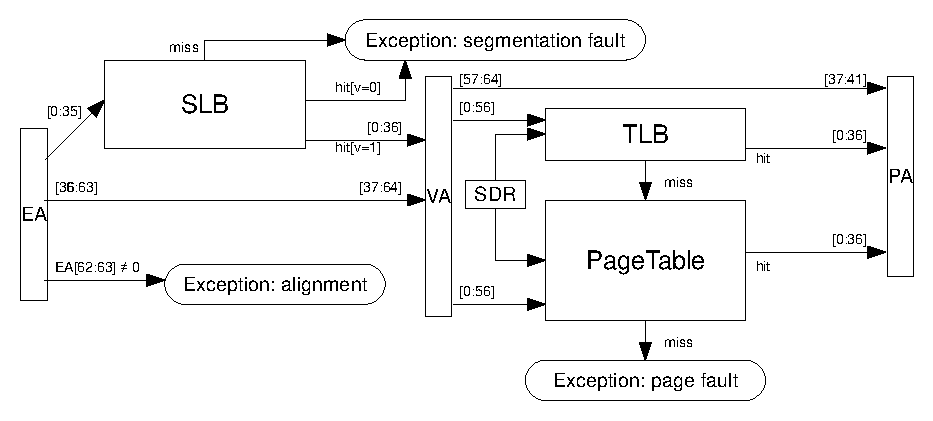
\includegraphics[width=\textwidth]{4.analysis/ppc_addrtrans}\\
  \caption{Трансляция адреса в PowerPC}\label{fig:ppc_address_translation}
\end{figure}


\section{Генерация тестов для архитектуры IA-32}\label{sec:ia32_application}

IA-32 --- это архитектура, разрабатываемая компанией Intel. Документация по
архитектуре IA-32 представлена книгой IA-32 Intel® Architecture
Software Developer’s Manual (в пяти томах)~\cite{IA32}. Второй и третий тома \\(Instruction Set Reference) содержат определения инструкций. Они действительно описываются в виде набора операций над битовыми строками на специальном псевдокоде. % (см. рисунок~\ref{fig:ia32_page}).

%\begin{figure}
%\framebox[0.93\textwidth][l]{\parbox{0.9\textwidth}{%
%
%\textbf{TEST—Logical Compare}\\
%
%\textbf{Description}\\
%Computes the bit-wise logical AND of first operand (source 1 operand) and the second operand
%(source 2 operand) and sets the SF, ZF, and PF status flags according to the result. The result is
%then discarded.\\
%
%\textbf{Operation}
%
%\texttt{TEMP <- SRC1 AND SRC2;}
%
%\texttt{SF <- MSB(TEMP);}
%
%\texttt{IF TEMP = 0}
%
%\hspace{1cm} \texttt{THEN ZF <- 1;}
%
%\hspace{1cm} \texttt{ELSE ZF <- 0;}
%
%\texttt{FI:}
%
%\texttt{PF <- BitwiseXNOR(TEMP[0:7]);}
%
%\texttt{CF <- 0;}
%
%\texttt{OF <- 0;}
%
%\texttt{(* AF is undefined *)}\\
%
%\textbf{Flags Affected}\\
%The OF and CF flags are set to 0. The SF, ZF, and PF flags are set according to the result (see
%the "Operation" section above). The state of the AF flag is undefined.
%}}
%\caption{Пример страницы документации системы команд архитектуры IA-32}\label{fig:ia32_page}
%\end{figure}

Четвертый и пятый тома (System Programming Guide) содержат описание подсистемы управления памяти в
микропроцессорах IA-32. Для работы с данными она содержит следующие устройства
(количественные характеристики приведены для микропроцессора Intel Pentium
Pro~\cite{PentiumPro}) :
\begin{itemize}
  \item \emph{кэш-память данных первого уровня (D-Cache-1)}:
        \begin{itemize}
            \item размер: 8 кБ;
            \item поля строк: тег адреса (ключ), данные (данные);
            \item битовая длина номера региона: 7 (наборно-ассоциативный);
            \item количество строк в регионе: 2;
            \item стратегия вытеснения \LRU;
        \end{itemize}

  \item \emph{кэш-память второго уровня (Cache-2)}:
        \begin{itemize}
            \item размер: в разных версиях 256 кБ, 521 кБ или 1 МБ;
            \item поля строк: тег адреса (ключ), данные (данные);
            \item битовая длина номера региона: от 11 до 13 в разных версиях
(наборно-ассоциативный);
            \item количество строк в регионе: 4;
            \item стратегия вытеснения \LRU;
        \end{itemize}

  \item \emph{TLB (D-TLB)}:
        \begin{itemize}
            \item поля строк: page number (ключ), page base address (данные),
флаги (данные);
            \item битовая длина номера региона: 4 (наборно-ассоциативный);
            \item количество строк в регионе: 4;
            \item стратегия вытеснения \LRU;
        \end{itemize}

  \item \emph{таблица страниц виртуальной памяти (PageTable)}:
    \begin{itemize}
        \item поля строк: page number (ключ), page base address (данные), флаги
(данные);
        \item битовая длина номера региона: 65;
        \item количество строк в регионе: 1;
        \item вытеснение программное;
        \item размер логического адреса: 48 бит;
        \item размер линейного адреса: 32 бит;
        \item размер физического адреса: 32 бита;
    \end{itemize}


  \item \emph{таблица дескрипторов сегментов (SDT)}:
        \begin{itemize}
            \item поля строк: segment selector (ключ), база (данные), флаги
(данные);
            \item битовая длина номера региона: 13;
            \item количество строк в регионе: 1;
            \item вытеснение программное;
        \end{itemize}
\end{itemize}

Другие устройства для обращения в память не используются.

\begin{figure}[h] \center
  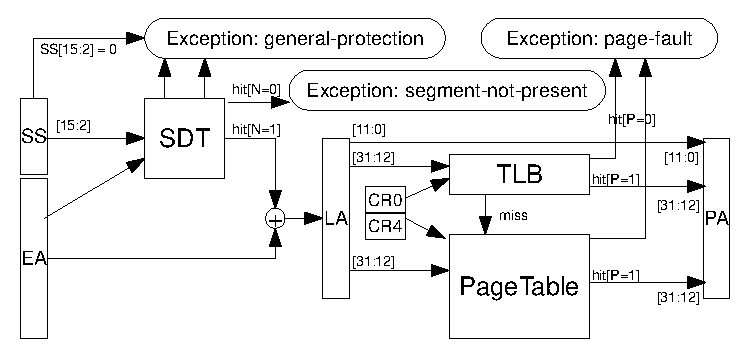
\includegraphics[width=0.9\textwidth]{4.analysis/ia32_addrtrans}\\
  \caption{Трансляция адреса в IA-32}\label{fig:ia32_address_translation}
\end{figure}

Осталось показать, что трансляция адресов также может быть представлена в виде отношений на битовых строках и обращений к таблицам. Обычное выполнение обращения в память в IA-32 следующее:
\begin{enumerate}
    \item на основе аргументов инструкции обращения к памяти формируется \emph{логический адрес} (SS:EA);
    \item заменой в логическом адресе номера сегмента на его адрес из SDT получается \emph{линейный адрес} (LA);
    \item либо линейный адрес трактуется как физический, либо заменой в линейном адресе номера виртуальной страницы на номер фрейма физической памяти получается физический адрес (PA);
    \item по физическому адресу, если нужно, осуществляется обращение в кэш-память или обращение в оперативную память.
\end{enumerate}

В зависимости от состояния управляющих регистров возможны следующие варианты трансляции адреса:
\begin{itemize}
  \item real-address mode (трансляция выключена) --- физический адрес равен линейному, линейный адрес вычисляется по логическому без обращения к каким-либо таблицам;
  \item protected mode --- режим с трансляцией адреса через таблицу страниц (см. рис.~\ref{fig:ia32_address_translation}).
\end{itemize}



\section{Экспериментальная реализация програм-\\много средства для генерации тестовых программ}

Был реализован прототип программного средства для генерации тестовых программ. Для проведения экспериментов к нему был добавлен генератор тестовых шаблонов. Компоненты прототипа программного средства для генерации тестовых программ следующие: %(см. рисунок~\ref{fig:activities}):
%\begin{figure}[h] \center
%  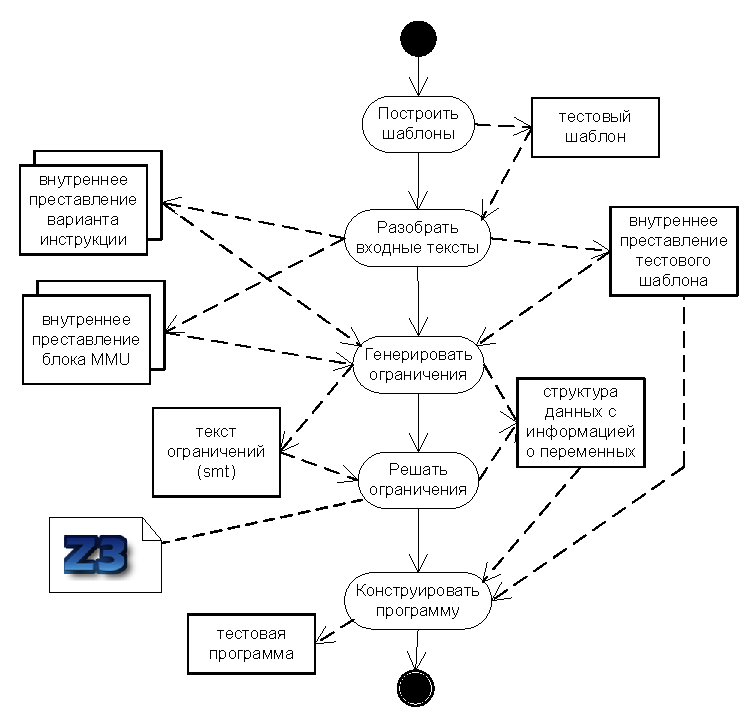
\includegraphics[width=0.7\textwidth]{3.impl/activities1}\\
%  \caption{Диаграмма деятельностей по генерации тестовых программ}\label{fig:activities}
%\end{figure}
\begin{enumerate}
  \item генератор тестовых шаблонов;
  \item синтаксический анализатор исходных текстовых данных; прототип генератора тестовых программ принимает на вход тексты в виде xml, создает внутреннее представление шаблона, моделей устройств, моделей вариантов исполнения инструкций для других компонентов;
  \item генератор (текстов) ограничений на основе описанных в разделах~\ref{sec:constraints_generation_section} и \ref{sec:usefulness_functions} методов генерирует тексты ограничений в формате SMT-LIB~\cite{SMT}; этот формат поддерживается большинством SMT-решателей ограничений, что делает возможным использовать разные внешние решатели ограничений и сравнивать их производительность применительно к генерируемым ограничениям; кроме того генератор ограничений строит структуры, хранящие семантическую информацию о переменных в ограничениях;
  \item обертка решателя ограничений вызывает внешний решатель ограничений, считывает результат его работы, извлекает из этого результата значения переменных и сохраняет эти значения в созданной генератором текстов ограничений структуре;
  \item конструктор текстов тестовых программ строит тексты тестовых программ на основе внутреннего представления шаблона и значений переменных.
\end{enumerate}

Часть компонентов зависит от тестируемого микропроцессора, а часть компонентов независима. К первым относятся конструктор текстов тестовых программ, поскольку он использует особенности, специфичные для отдельных микропроцессоров или семейств микропроцессоров. Остальные компоненты не зависят от тестируемого микропроцессора и без изменений могут быть использованы в генераторах тестовых программ других микропроцессоров.

В реализованном прототипе синтаксический анализатор моделей, генератор текстов ограничений, обертка решателя ограничений были написаны на Ruby (порядка 2000 строк). В качестве решателя ограничений был выбран инструмент Z3~\cite{Z3}, поскольку этот инструмент имеет одни из лучших показателей эффективности по сравнению с другими аналогичными инструментами.

В качестве архитектуры тестируемых микропроцессоров для экспериментов был выбран MIPS64, отчасти из-за наличия готовых компонентов для проведения тестирования и моделей микропроцессоров. Конструктор тестовых программ для MIPS64 был реализован на Java (порядка 500 строк). Типичные размеры описаний вариантов исполнения инструкций --- 100 строк (в представлении на xml). Типичный размер описаний устройств --- 20 строк (в представлении на xml). Эти описания подготавливались вручную на основе документации по микропроцессору.

\section{Эксперименты по оценке допустимой сложности тестовых шаблонов}\label{sec:templates_estimation}

%эксперименты с длинами и временем генерации/процентом успешной
%генерации. Показать, что допустимая длина действительно увеличивается!

Хотя теоремы~\ref{mirror_correctness}, \ref{mirror_fullness_none} и \ref{mirror_fullness} (о корректности и полноте методов генерации ограничений) гарантируют, что тестовая программа для тестового шаблона существует тогда и только тогда, когда совместна система ограничений (при существенно вытесняющей стратегии вытеснения). Однако не всегда совместность систем ограничений можно определить за ограниченное время (поскольку требуется строить тестовые программы для определенного количества тестовых ситуаций за вполне ограниченное, выделенное на это время в рамках проектов по тестированию моделей микропроцессоров). Из очевидных соображений чем <<сложнее>> тестовый шаблон, тем больше требуется времени на построение тестовой программы по нему (и определения того, что тестовая программа существует). Под сложностью понимается степень зависимости параметров тестового шаблона. Чем больше зависимостей, тем сложнее тестовый шаблон. Чем меньше зависимостей, тем продуктивнее будет воспользоваться более простыми целенаправленными методами получения тестовых программ, нежели предлагаемыми в диссертации. Поэтому важно иметь оценку допустимой <<сложности>> тестовых шаблонов, исходя из реальных решателей и реальных тестируемых микропроцессоров.

Для получения таких оценок был проведен ряд экспериментов. В экспериментах тестовые шаблоны состояли из инструкций загрузки и сохранения данных в памяти. В каждой инструкции должна была выполняться трансляция адреса через TLB (с использованием D-TLB) и затем обращение в основную память через кэш-память первого уровня. Вариант исполнения инструкций загрузки и сохранения задавался парой параметров: успешность обращения в TLB и успешность обращения в кэш-память. Модель вариантов инструкции загрузки LD приведена в приложении~\ref{sec:xml}. Рассматривались все длины тестовых шаблонов от 2 до 16. Для каждой длины проводились эксперименты для разных моделей микропроцессоров: они отличались ассоциативностью кэш-памяти. Использовались значения ассоциативности --- 2, 4, 8 и 16. При фиксированной длине шаблона и ассоциативности кэш-памяти случайным образом генерировался тестовый шаблон (т.е. случайным образом выбирались зависимости аргументов инструкций и варианты исполнения для инструкций). Количество тестовых шаблонов имело порядок тысяч шаблонов. Далее в этом разделе проводится статистический анализ для обоснования выбранного количества тестовых шаблонов для экспериментов.

Эксперименты проходили на компьютере AMD Athlon64 3200+ 2ГГц с 1ГБ оперативной памяти.

Рисунки~\ref{fig:success_experiment} и~\ref{fig:time_experiment} представляют результаты экспериментов. На рисунке~\ref{fig:success_experiment} по оси абсцисс отложена длина тестового шаблона, а по оси ординат отложена доля шаблонов заданной длины из случайно сгенерированного набора шаблонов заданной длины, для которых была построена тестовая программа за время, меньшее чем 60 секунд или был получен сигнал о том, что тестовой программы не существует (эта доля и названа <<успешностью>>). Если время работы решателя ограничений превышало 60 секунд, построение тестовой программы обрывалось. На рисунке~\ref{fig:time_experiment} по оси абсцисс отложена длина тестового шаблона, а по оси ординат отложено среднее арифметическое времени генерации тестовой программы для тестового шаблона заданной длины из случайно сгенерированного набор шаблонов заданной длины. Более точно, среднее время определения того, что шаблон <<является несовместным>> (для него не может быть теста вовсе) или совместным с построением соответствующей ему тестовой программы. Эксперименты показали, что это время варьируется от 1 до 30 секунд для тестовых шаблонов длиной от 2 до 14 инструкций.

%Замечено, что большую часть времени построения тестовой программы занимало разрешение ограничений.


\begin{figure}[p] \center
\parbox[t]{0.9\textwidth}{
  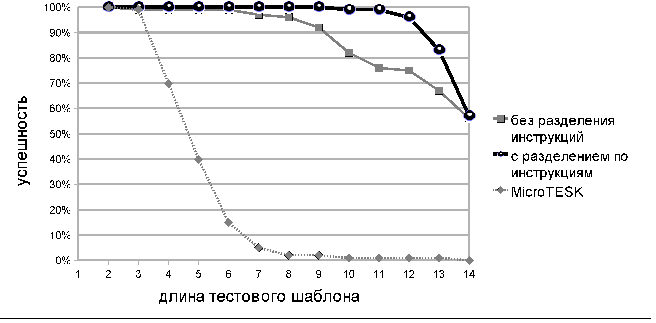
\includegraphics[width=0.9\textwidth]{4.analysis/success_exprmnt}%
\caption{Доля тестовых шаблонов, для которых удалось построить тестовую программу за 60с или определить их несовместность}\label{fig:success_experiment}
}

\vspace{1.5cm}

\parbox[t]{0.9\textwidth}{
  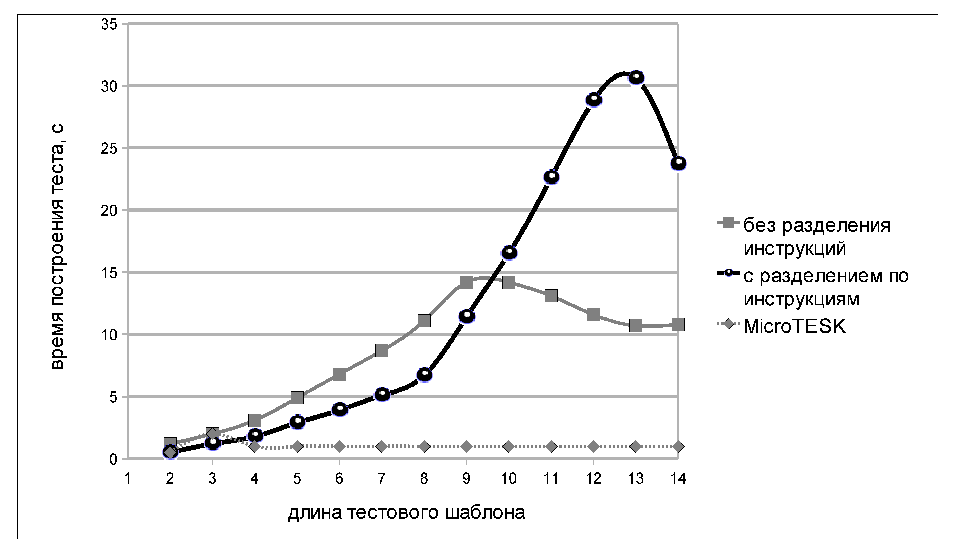
\includegraphics[width=0.9\textwidth]{4.analysis/time_exprmnt}
  \caption{Среднее время построения тестовой программы / определения несовместности тестового шаблона}\label{fig:time_experiment}
}
\end{figure}

В первой серии экспериментов (их результаты отражены на рисунках линиями с
квадратиками) генерация ограничений делалась для всего тестового шаблона.
Оказалось, что до некоторой длины шаблона (значит, и теста) (8-9) метод работает
успешно практически для всех тестовых шаблонов (97\%-100\%). При дальнейшем
увеличении длины шаблона начинает уменьшаться доля шаблонов, для которых удается
построить тест (по 5-10\% при увеличении длины теста). Тем самым при длине теста
порядка 14-15 уже для половины шаблонов решатель ограничений не успевает за 60
секунд обработать тестовый шаблон (и построить тест). В результате анализа использованных в
экспериментах тестовых шаблонов был сделан вывод, что для большинства из них
(60-70\%) тестов не может быть вовсе, так как в этих шаблонах имеются пары расположенных подряд обращений
по одинаковым адресам, при этом первое обращение --- успешное или неуспешное, а второе --- успешное. Для таких шаблонов не существует тестовых программ (поскольку в результате промаха данные помещаются в таблицу и при повторном обращении к ним должно происходить только попадание, а не промах).

Поскольку эта ситуация стала по сути следствием случайного выбора тестовых
шаблонов, то в следующей серии экспериментов перед запуском генерации
ограничений была вставлена процедура, отсеивающая априори несовместные тестовые
шаблоны (т.е. такие, для которых не может существовать тестов вовсе). Кроме того
обращения в кэш-память были поделены на группы на основе одинаковых имен
аргументов и для этих групп генерировались ограничения (грубо говоря, к шаблону
добавлялось требование обращения по разным именам аргументов в разные регионы,
если это не противоречило шаблону). Результаты этой второй серии экспериментов
отражены на рисунках~\ref{fig:success_experiment} и \ref{fig:time_experiment}
линией с кружками. Из них следует, что примененные изменения позволили
дополнительно увеличить на несколько единиц допустимый размер тестового шаблона.

Для каждой пары (длина шаблона, ассоциативность) было сгенерировано 1000
тестовых шаблонов. Насколько можно доверять полученным в экспериментах
результатам на таком количестве тестовых шаблонов? Для ответа на этот вопрос воспользуемся аппаратом теории
вероятностей. Пусть $N$ --- количество испытаний. Одно испытание заключается в
следующем: сначала случайным образом строится тестовый шаблон, затем генерируются
для него ограничения и, наконец, они разрешаются. Испытание заканчивается успешно, если за отведенное время (60с) решатель ограничений <<построил тест>>, и неуспешно, если не успел <<построить>>.
Обозначим  $\xi_i$, $i = 1, 2, \dots, N$, случайные величины, соответствующие
успешности испытаний. Их областью значений будет множество $\{0, 1\}$. Эти
случайные величины независимы и одинаково распределены (обозначим $p =
\mathsf{P}\{\xi_i = 1\}$). Поэтому применим \emph{закон больших чисел}, согласно
которому $\frac{\sum_{i=1}^N \xi_i}{N} \sim p$ при <<больших>> $N$. Более точно, для любых
положительных $\varepsilon$ и $\delta$ найдется число $N^*$, что для всех $N > N^*$ будет
выполнено $\mathsf{P}\{|\frac{\sum_{i=1}^N \xi_i}{N} - p | \geq \varepsilon\} \leq \delta$. $\varepsilon$ --- это допустимое отклонение в оценке результата экспериментов (т.е. оценке $p$). $\delta$ показывает, насколько можно доверять полученному результату экспериментов. Поскольку $\sum \xi_i$ распределена по биномиальному закону ($\mathsf{P}\{\sum_{i=1}^N \xi_i = m\} = \binom{N}{m} p^m (1{-}p)^{N{-}m}$), то для вероятности отклонения более, чем на $\varepsilon$, справедлива следующая формула: $$\sum_{m = 0}^{(p-\varepsilon)N} \binom{N}{m} p^m (1{-}p)^{N{-}m} + \sum_{m = (p+\varepsilon)N}^N \binom{N}{m} p^m (1{-}p)^{N{-}m} \leq \delta$$ Эта формула позволяет оценить $\delta$ при разных $p$, зная $\varepsilon$ и $N$.

Итак, для каждого $n \in \{2,3\}$ ($n$ --- длина тестового шаблона) было сгенерировано по $B = 1000$ тестовых шаблонов. При этом получилось $p \in [0.9, 1.0]$. Если взять допустимое отклонение от истинного значения $\varepsilon = 0.02$ (2\%) (что вполне допустимо, т.к. отклонение в 2\% не сильно изменит результат эксперимента), то вероятность ошибиться в этом случае была бы не более $\delta = 0.03$, т.е. 3\%, что тоже вполне допустимо. Для $n \in \{4, 5, 6, 7\}$ было сгенерировано по $N = 2000$ тестовых шаблонов (для $w \in \{2,4\}$). Если взять $\varepsilon = 0.02$ (2\%), то для $p \in [0.9, 1.0] ~ \delta{=}0.003$, т.е. $0.3\%$, т.е. ошибка в этом случае еще меньше. И, наконец, для $n \in \{8, 9, ..., 14\}$ было сгенерировано по $N = 3000$ тестовых шаблонов, что при $\varepsilon = 0.02$ и $p \in [0.5, 1.0]$ дает $\delta = 0.02$, т.е. всего 2\%. Таким образом, вероятность ошибки в проведенных экспериментах невелика.

Проведенные эксперименты позволяют произвести сравнение с инструментом
MicroTESK~\cite{MicroTESK}. Этот инструмент был успешно применен для построения
тестов по всевозможным тестовым шаблонам из 2-3 инструкций~\cite{vorobyev}. При
увеличении длины тестового шаблона (и, соответственно, его <<сложности>>) удается
строить тесты для всё меньшего количества шаблонов. Что и отражено на
рисунках~\ref{fig:success_experiment} и \ref{fig:time_experiment} линиями с
ромбами. Напротив, как показывают эксперименты, предложенные методы позволяют
строить тесты по шаблонам из 8-11 инструкций обращения к памяти. Допустимая
длина шаблонов может быть еще больше, если кроме инструкций обращения к памяти в
шаблоне используются и другие инструкции (например, арифметические).

\section{Сравнение с Genesys-Pro}

В разделе~\ref{sec:templates_estimation} было произведено сравнение предлагаемых в диссертации методов генерации тестовых программ с методами, реализованными в инструменте
MicroTESK~\cite{MicroTESK}. В этом разделе будет произведено сравнение с другим
инструментом целенаправленной генерации тестовых программ --- Genesys-Pro~\cite{GenesysPro} --- по организации генератора, производительности, организации входных данных и др. Сравнить
по эффективности экспериментальным способом с Genesys-Pro не удается, поскольку этот инструмент не распространяется за пределы IBM. Сравнение по другим характеристикам проводилось на основе  публикаций~\cite{GenesysPro2004Innovations, GenesysSolver}.

Технологически подготовка к генерации тестов с использованием Genesys-Pro выглядит следующим образом:
\begin{enumerate}
    \item подготовить Architectural simulator --- эталонный симулятор микропроцессора (интерпретатор инструкций микропроцессора);
    \item подготовить Testing knowledge --- комплект ограничений на аргументы инструкций, задающих <<интересные для тестирования>> соотношения значений и аргументов;
    \item подготовить Architectural model --- описание системы команд тестируемого микропроцессора с указанием набора атрибутов (атрибут содержит имя и поля) и ограничений значений полей атрибутов для каждой инструкции (по сути, описание предусловия инструкции и вычисляемой инструкцией функции в виде ограничений); пример описания инструкции загрузки из памяти Load-Word изображен на рисунке~\ref{fig:GenesysProArchitecturalModel} (в овалах Source, Base, Target и другие --- атрибуты инструкции (среди них Base, Target, Displacement --- аргументы инструкции), Family, Data, Data и другие --- поля атрибутов, линии с точками между овалами --- ограничения, формула, задающая ограничение, написана под линией); для описания трансляции адреса предлагается метод DeepTrans~\cite{DeepTrans} --- пример изображен на рисунке~\ref{fig:DeepTransExample} (овалы Initial, Exception, Final --- этапы трансляции адреса, Virtual Address, Access Type, Real Address и другие --- атрибуты этапов, PageTranslation --- обращение к таблице трансляции, Entry Data, Real Page Number и другие --- атрибуты строки таблицы страниц, прямоугольник рядом PageTranslation задает предикат соответствия строки таблицы страниц атрибутам Initial (Table Match Condition) и предикат соответствия строки таблицы страниц атрибутам Final (Table Internal Relations));
    \item подготовить Test template --- тестовый шаблон; в нем задается последовательность инструкций тестовой программы и, возможно, ограничения из Testing Knowledge;
        %пример тестового шаблона приведен на рисунке~\ref{fig:genesysPro_template}: Var определяет переменные, Bias задает вероятности возникновения ситуаций (<<resource\_dependency(GPR)>> должен встретиться как минимум в 30\% тестовых программ, сгенерированных по данному тестовому шаблону, <<alignment(4)>> --- в 50\%), Instruction задает очередную инструкцию тестовой программы, with Bias задает вероятность ;
    \item подготовить или использовать имеющийся решатель ограничений;
%    \item запустить Genesys-Pro с подготовленными моделями.
\end{enumerate}
%% я понимаю, что такую последовательность шагов нельзя называть
%% технологической, ибо непоятно
%% 1) как выбирать Testing knowledge - что туда включать, а что нет; наверняка,
%% есть некое понимание того, что хочется протестировать; это понимание
%% должно быть формализовано (модель покрытия) и на его основе уже решать,
%% что включать в Testing knowledge, а что нет;
%% 2) не описано, как анализировать результаты Genesys-Pro: всё ли он сделал или
%% нет, надо ли дорабатывать то, что он генерирует? Надо ли как-то иначе
%% формулировать модели с шагов 1-3 для того, чтобы тесты были построены
%% целиком. И что значит "целиком"? Нет ведь модели покрытия!

%\begin{figure}[h] \center
%  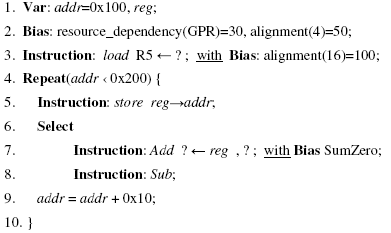
\includegraphics[width=0.6\textwidth]{4.analysis/genesys_tmpl}
%  \caption{Пример тестового шаблона в нотации инструмента Genesys-Pro}\label{fig:genesysPro_template}
%\end{figure}

\begin{figure}[h] \center
  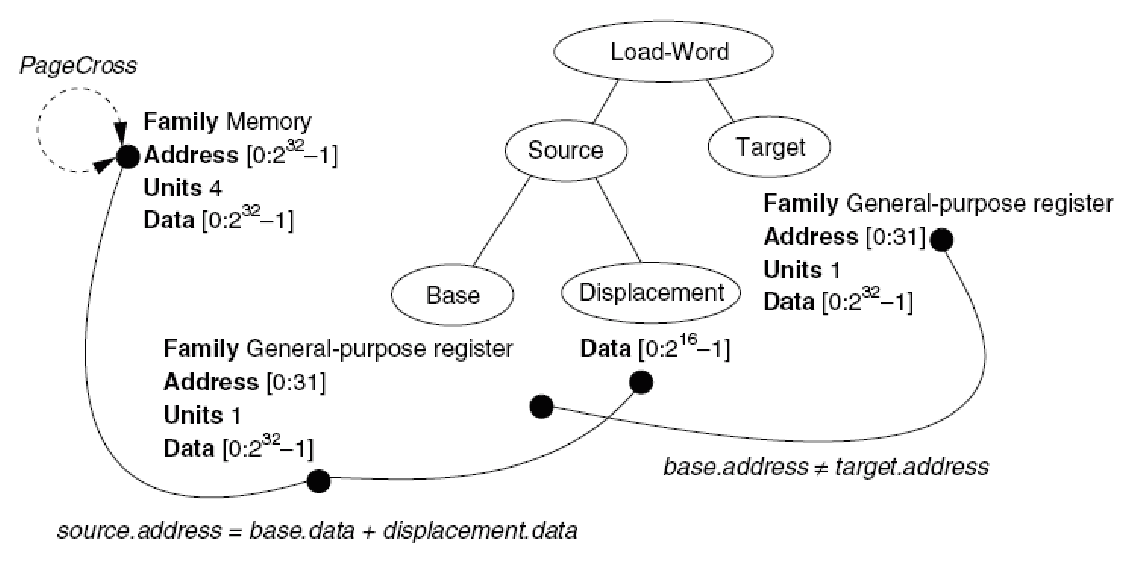
\includegraphics[width=0.8\textwidth]{4.analysis/arch-model}
  \caption{Architectural model для инструкции
Load-Word}\label{fig:GenesysProArchitecturalModel}
\end{figure}

\begin{figure}[h] \center
  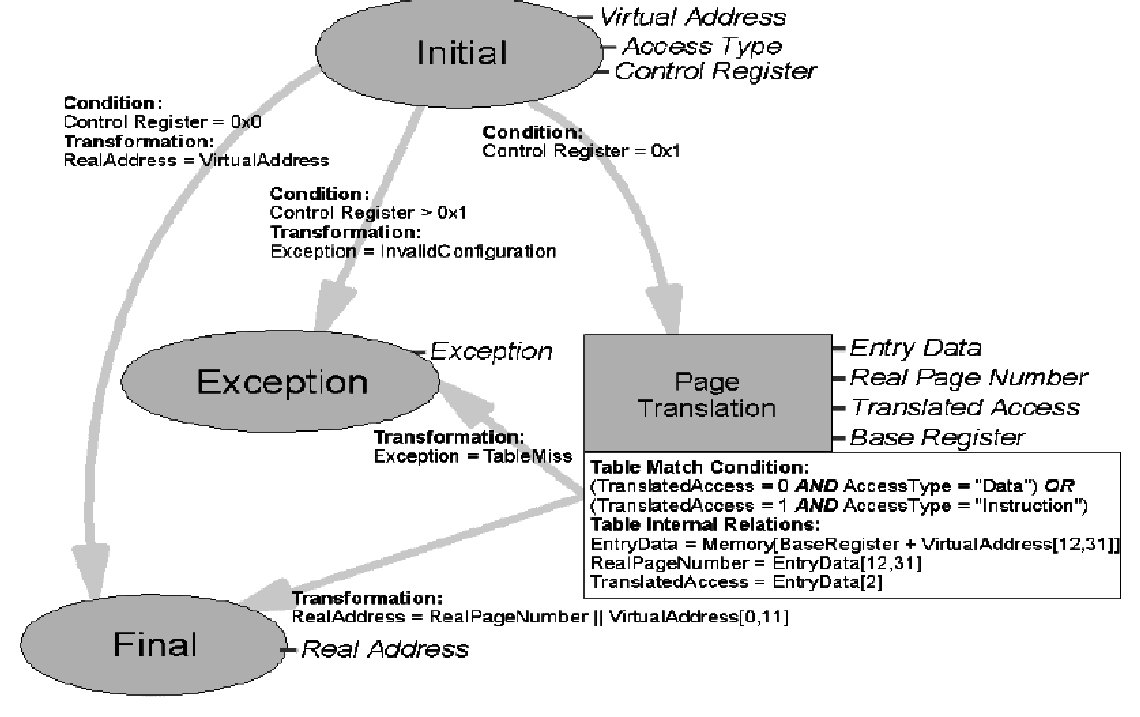
\includegraphics[width=0.8\textwidth]{4.analysis/deeptrans}
  \caption{Пример описания трансляции адреса по методу DeepTrans в инструменте Genesys-Pro}\label{fig:DeepTransExample}
\end{figure}

%\begin{figure}[h] \center
%  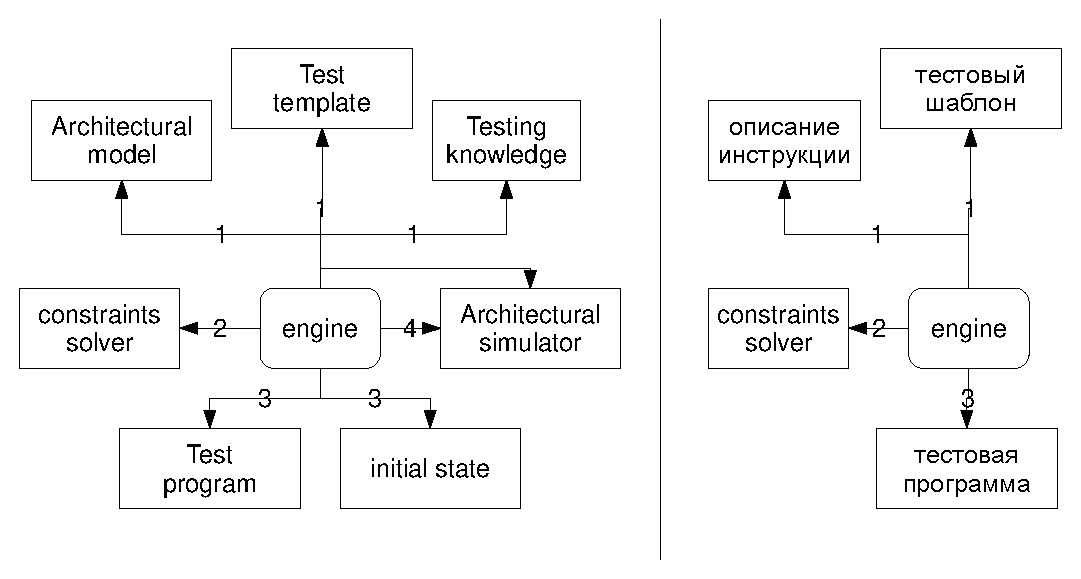
\includegraphics[width=\textwidth]{4.analysis/g-pro}
%  \caption{Genesys-Pro (слева) и предлагаемый в диссертации генератор (справа)}\label{fig:GenesysProScheme}
%\end{figure}

Genesys-Pro строит тестовую программу, чередую построение очередной инструкции и симуляцию этой инструкции, при этом каждый раз уточняя начальное состояние микропроцессора. Если построить очередную инструкцию невозможно (не удается подобрать параметры), происходит возврат на шаг назад и перегенерируется предыдущая инструкция. Аргументы каждой инструкции должны в текущем состоянии модели микропроцессора удовлетворять ограничениям из Architectural model и Testing knowledge. Для получения таких аргументов составляются системы ограничений и разрешаются встроенным решателем ограничений.

% т.е. получается, симулятор должен быть каким-то особенным, чтобы уметь
% работать из неполного состояния? (с lazy-значениями 'X') поскольку не
% всё начальное состояние построено перед
% первой инструкций и достраивается в процессе построения теста

Тем самым у предлагаемого в диссертации подхода, моделей и методов имеются следующие сходства с Genesys-Pro:
\begin{itemize}
    \item присутствуют способы указания ограничений на значения аргументов отдельных инструкций в тестовом шаблоне (здесь эти ограничения описываются в  виде вариантов исполнения инструкций, а в Genesys-Pro эти ограничения описываются в тестовом шаблоне и Testing know-ledge);
    \item тестовый шаблон и микропроцессор описываются декларативным образом;
    \item оба подхода относятся к <<моделеориентированным>> --- в таких подходах есть генератор, который принимает на вход модель микропроцессора; альтернативой могла быть технология, в которой по модели вручную приходилось бы реализовывать на каком-нибудь языке программирования ряд специальных компонентов (в том числе учитывающие особенности модели микропроцессора и тестового шаблона), которые вместе дадут генератор тестовых программ;
    \item использование техники ограничений (constraints) для построения тестовых программ;
    \item сходные идеи есть и в методе описания трансляции адресов: в обоих случаях -- это декларативное описание, в обоих случаях описывается то, как формируются виртуальные/физические адреса; в обоих случаях описание трансляции основывается на представлении содержимого устройств подсистемы управления памяти в виде массивов данных, для которых задается ряд атрибутов (в том числе в Genesys-Pro есть аналог предиката keyMatch).
\end{itemize}

Имеются следующие отличия подходов:
\begin{itemize}
    \item разные принципы построения тестовых программ и ограничений; Genesys-Pro строит ее по одной инструкции и формулирует ограничения только для одной очередной инструкции; напротив, в предлагаемом методе ограничения строятся для всего тестового шаблона целиком;
    \item разные методы построения ограничений; при генерации системы ограничений Genesys-Pro существенно использует известную часть состояния микропроцессора (от Architectural simulator); напротив, в предлагаемом методе построения ограничений состояние микропроцессора неизвестно вообще; это приводит к ограничениям разной природы;
    \item Genesys-Pro предполагает для инструкции раздельное описание вычисляемой функции и ограничений на входные данные; в предлагаемом методе эти описания оформляются вместе;
%    \item язык описания тестовых шаблонов в Genesys-Pro позволяет компактно описать длинные тестовые программы (из сотен тысяч инструкций), кроме того этот язык позволяет описывать классы тестовых шаблонов;
    \item разный способ описания функциональности инструкций; у Genesys-Pro --- это система ограничений на атрибуты инструкции и ее аргументы, а здесь --- это последовательность операторов;
    \item Genesys-Pro рассчитан на подготовку специальных решателей ограничений (из-за специфики его систем ограничений); напротив, в предлагаемом методе используются сторонние решатели ограничений и отдельно подготавливать их не нужно.
\end{itemize}

Преимущества и недостатки по сравнению с Genesys-Pro следующие:
\begin{itemize}
%    \item Genesys-Pro поддерживает тестовые шаблоны, задающие цепочки инст{-}рукций из сотен и тысяч инструкций, т.е. он обладает преимуществом по длине генерируемых тестовых программ; однако такие тестовые шаблоны содержат существенно меньше зависимых параметров, нежели сотни и тысячи, поскольку шаблоны представляют собой итерацию конечных небольших последовательностей зависимых инструкций (см. рисунок~\ref{fig:genesysPro_template});
    \item преимуществом предлагаемого в диссертации подхода является меньшая трудоемкость подготовки генератора тестовых программ (как минимум, потому что не нужно разрабатывать решатель ограничений);
    \item возможность построения ограничений целиком для всего шаблона в предлагаемых методах дает преимущество перед построением по одной инструкции в Genesys-Pro по времени построения тестовой программы, например, для тестового шаблона с такой последовательностью инструкций: одна из инструкций вытесняет специальные данные (например, их тег адреса делится на 16) --- если Genesys-Pro не обеспечит таких данных, ему придется делать возвраты к предыдущим инструкциям (причем не на одну инструкцию, а несколько).
\end{itemize}

%Genesys-Pro чётко разделяет свойства аргументов
%инструкции и свойства результата инструкции, соотношение между ними
%задается не с помощью ограничений (т.е. не декларативным способом),
%а в виде алгоритма (т.е. императивным способом).
%
%Другой особенностью Genesys-Pro является то, что поддерживаемые им
%тестовые шаблоны зачастую не фиксируют последовательность инструкций
%(это позволяет строить более простые ограничения, потому как
%генерируемая последовательность инструкций может по ходу генерации
%подстраиваться под уже сгенерированные инструкции со
%сгенерированными значениями аргументов, под состояние
%микропроцессора, в которое привели сгенерированные инструкции).
%
%Выразительный язык Genesys-Pro для описания ограничений однако
%содержит такие нетривиальные конструкции, как явное использование
%элементов массивов данных, что требует для разрешения продвинутый
%решатель CSP, в том числе и заточенный под особенности генерации
%тестовых данных для тестовых шаблонов (как минимум такие ограничения
%могут включать битовые операции). Подобный решатель был разработан в
%IBM для инструмента Genesys-Pro~\cite{GenesysSolver}. Однако
%создание такого решателя -- отдельное сложное исследование, которое
%не входило в цели данного исследования. В данной работе было принято
%решение использовать доступные существующие решатели (не обязательно
%CSP) и сосредоточиться на упрощении генерируемых ограничений для
%некоторых частных случаев архитектур.
%
%%\begin{figure}[h]
%%\parbox{0.5\textwidth}{ \centering
%%  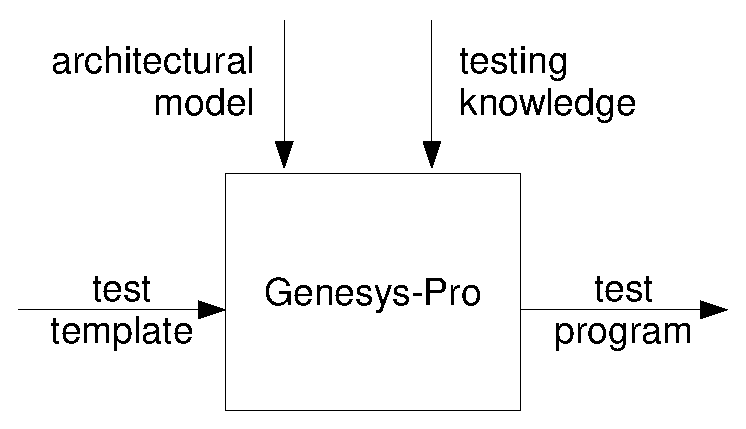
\includegraphics[width=0.45\textwidth]{3.impl/genesys-pro}
%%} \vline
%%\parbox{0.5\textwidth}{ \centering
%%  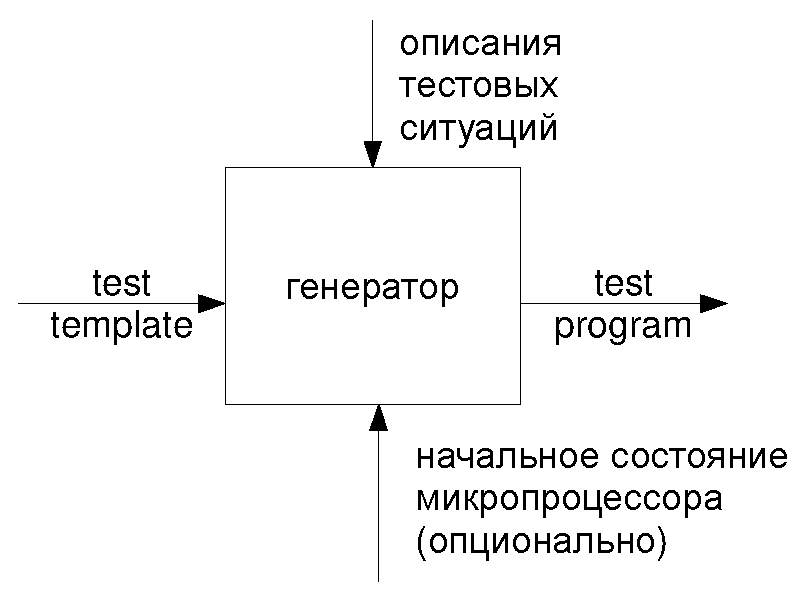
\includegraphics[width=0.45\textwidth]{3.impl/mygen}
%%}
%%\caption{Сравнение с Genesys-Pro}\label{comparison_genesyspro}
%%\end{figure}
%
%В отличие от Genesys-Pro в предлагаемом инструменте описание
%семантики инструкций задается в едином виде -- в виде описаний
%тестовых ситуаций~\cite{my_syrcose_2008, my_isp_2008}. Каждая
%тестовая ситуация описывает не только ограничение на свои аргументы,
%но и результат исполнения инструкции \emph{при данном ограничении на
%аргументы} инструкции декларативным образом. В функции, которую
%реализует инструкция, выделяются отдельные \emph{ветви
%функциональности}, ситуации различного поведения инструкций, каждая
%ветвь функциональности становится отдельной тестовой ситуацией.
%Например, инструкция целочисленного сложения ADD может быть
%исполнена либо точно, либо с возникновением переполнения. Поэтому у
%этой инструкции можно выделить 2 ветви функциональности (точное
%исполнение и исполнение с переполнением), каждая ветвь дает свою
%тестовую ситуацию.

\section{Сравнение с работами Intel}

В ряде публикаций~\cite{MicroFORMAL} описывается инструмент MicroFORMAL, разрабатываемый в Intel. Он используется для некоторых задач формальной верификации разрабатываемых микропроцессоров (в частности, для проверки обратной совместимости). В рамках этой работы требуется описывать поведение микропроцессоров, формализовывать функциональность инструкциЙ. Авторы статей разработали \emph{IRL-представление} микрокода (IRL --- Intermediate Representation Language). Спецификация на IRL описывает функциональность инструкции и побочный эффект (изменение <<внешних>> переменных). Ровно ту же цель преследуют и модели вариантов исполнения инструкций, предлагаемые в данной работе. Спецификация на IRL представляет собой последовательность операторов (эта же идея используется здесь).

IRL включает в себя управляющие операторы (\texttt{if}, \texttt{goto}), поскольку верификация с использованием спецификаций на IRL нацелена в первую очередь на верификацию потоков управления. В данной работе поток управления не предполагает подобных операторов.

IRL позволяет описывать инструкции обращения к памяти. Однако в IRL используется лишь <<плоская>> модель памяти (т.е. память рассматривается как одномерный массив ячеек) с возможностью обращения <<по индексу>>. Напротив, модели инструкций, предлагаемые в данной работе, позволяют описывать работу с памятью более детально, с указанием успешности обращений в различные устройства подсистемы управления памяти.


% !Mode:: "TeX:UTF-8"
\chapter*{Заключение}
\addcontentsline{toc}{chapter}{Заключение}

Основные научные и практические результаты, полученные в
диссертационной работе и выносимые на защиту, состоят в следующем:

\Results

%Основные результаты диссертации являются новыми, получены автором самостоятельно.



%% TODO:
%% 6) проверить, что в pdf корректно отображается символ N натуральных чисел
%%           шрифт! на страницах 63, 68, 87, 130, 132
%% 18) опять обрезался верх картинки (с.116, 121) ??
%% 21) проверить поля в pdf
%%

\pagebreak
\appendix
% % !Mode:: "TeX:UTF-8"
\chapter{Таблицы ограничений}
%\addcontentsline{toc}{chapter}{Приложение А: Таблицы ограничений}

\begin{table}[h] \small
\begin{tabular}{|c|c|c|c|}
\hline  & \centering случай &
\begin{tabular}{c}переменная\\перебора\end{tabular} & система \\
\hline \hline \multirow{10}{*}{\rotatebox{90}{кэш-попадание}} &
\makecell[c{p{0.3\textwidth}}]{тегсет находится в начальном
состоянии буфера, к нему нет обращений до данной инструкции и он всё
ещё не вытеснен} & $\lambda \in L_0$ &
$\left\{\begin{array}{l} x = \lambda\\
x \notin \{x_1, ..., x_n\}\\
\bigwedge\limits_{x_m:\mbox{miss}}\sum\limits_{i=1}^W v_m(\xi_i) +
\sum\limits^{m-1}_{i=1} u_m(x_i) < W
\end{array}\right.
$ \\ \hhline{~|---} & \makecell[c{p{0.3\textwidth}}]{тегсет
находится в начальном состоянии буфера, к нему есть обращение до
данной инструкции и он всё ещё не вытеснен} & $\lambda \in L_0$ &
$\left\{\begin{array}{l} x = \lambda\\
x \in \{x_1, ..., x_n\}\\
\bigwedge\limits_{x_m:\mbox{miss}}\sum\limits^{m-1}_{i=1} u_m(x_i) <
W
\end{array}\right.
$ \\  \hhline{~|---} & \makecell[c{p{0.3\textwidth}}]{тегсет был
внесен одним из кэш-промахов и с того момента не вытеснен} & -- &
$\left\{\begin{array}{l}
x \in [x_1, ..., x_n]_{miss}\\
\bigwedge\limits_{x_m:\mbox{miss}}\sum\limits^{m-1}_{i=1} u_m(x_i) <
W
\end{array}\right.
$ \\ \hline \hline \multirow{20}{*}{\rotatebox{90}{кэш-промах}} &
\makecell[c{p{0.3\textwidth}}]{тегсет встречается впервые} & -- &
$\left\{\begin{array}{l} x \notin L_0\\
x \notin [x_1, ..., x_n]_{miss}\\
\end{array}\right.
$ \\ \hhline{~|---} & \makecell[c{p{0.3\textwidth}}]{тегсет ранее
был внесен одной из инструкций шаблона, затем вытеснен} & -- &
$\left\{\begin{array}{l}
x \in [x_1, ..., x_n]_{miss}\\
\bigvee\limits_{x_m : \mbox{miss}}\sum\limits^{m-1}_{i=1} u_m(x_i) \geqslant W\\
\end{array}\right.$ \\  \hhline{~|---} &
\makecell[c{p{0.3\textwidth}}]{тегсет находился в начальном
состоянии буфера и был вытеснен, к нему не было обращений в шаблоне}
& $\lambda \in L_0$ & $\left\{\begin{array}{l}
x = \lambda\\
x \notin \{x_1, ..., x_n\}\\
\bigvee\limits_{x_m : \mbox{miss}}\sum\limits^W_{i=1} v_m(\xi_i) + \sum\limits^{m-1}_{i=1} u_m(x_i) \geqslant W\\
\end{array}\right.
$ \\ \hhline{~|---} & \makecell[c{p{0.3\textwidth}}]{тегсет
находился в начальном состоянии буфера и был вытеснен, к нему было
обращение в шаблоне после последнего внесения в буфер} & $\lambda
\in L_0$ &
$\left\{\begin{array}{l} x = \lambda\\
x \in \{x_1, ..., x_n\}\\
\bigvee\limits_{x_m : \mbox{miss}}\sum\limits^{m-1}_{i=1} u_m(x_i) \geqslant W\\
\end{array}\right.
$ \\ \hline
\end{tabular}
\caption{Таблица систем уравнений в случае стратегии вытеснения
\PseudoLRU c использованием функций полезности}\label{plru_table}
\end{table}


\begin{landscape}
\begin{table}[p]\small
\begin{tabular}{|c|c|c|c|c|c|}
\hline  & \centering случай &
\begin{tabular}{c}переменная\\перебора\end{tabular} & система &
\begin{tabular}{c}функция полезности\\для кэш-попадания\end{tabular} &
\begin{tabular}{c}функция полезности\\для кэш-промаха\end{tabular} \\
\hline \hline \multirow{10}{*}{\rotatebox{90}{кэш-попадание}} &
\makecell[c{p{0.38\textwidth}}]{тегсет находится в начальном
состоянии буфера, к нему нет обращений до данной инструкции и он всё
ещё не вытеснен} & $\lambda_\delta \in D$ &
$\left\{\begin{array}{l} x = \lambda_\delta\\
x \notin \{x_1, ..., x_n\}\\
\sum\limits^n_{i=1} u(x_i) \leqslant w - \delta
\end{array}\right.
$ &
\begin{tabular}{c}
$x_i \in \{ \lambda_{\delta+1}, ..., \lambda_w\}$\\
$\wedge~x_i \notin \{x_1, ..., x_{i-1}\}$
\end{tabular}
& $R(x_i) = R(x)$
\\ \hhline{~|-----}
& \makecell[c{p{0.38\textwidth}}]{тегсет находится в начальном
состоянии буфера, к нему есть обращение до данной инструкции и он
всё ещё не вытеснен} & $\lambda_\delta \in D$ &
$\left\{\begin{array}{l} x = \lambda_\delta\\
x \in \{x_1, ..., x_n\}\\
\sum\limits^n_{i=1} u(x_i) < w
\end{array}\right.
$ &
\begin{tabular}{c}
$x \notin \{x_i, ..., x_n\}~\wedge$\\
$x_i \in \{ \lambda_{\delta+1}, ..., \lambda_w\}$\\
$\wedge~x_i \notin \{ x_{i+1}, ..., x_n\}$\\
\end{tabular}
&
\begin{tabular}{c}
$x \notin \{x_i, ..., x_n\}$\\
$\wedge~R(x_i) = R(x)$\\
\end{tabular}
\\  \hhline{~|-----}
& \makecell[c{p{0.38\textwidth}}]{тегсет был внесен одним из
кэш-промахов и с того момента не вытеснен} & -- &
$\left\{\begin{array}{l} x \in [x_1, ..., x_n]_{miss}\\
\sum\limits^n_{i=1} u(x_i) < w
\end{array}\right.
$ &
\begin{tabular}{c}
$x \notin \{x_i, ..., x_n\}$\\
$\wedge~R(x_i) = R(x)~\wedge$\\
$x_i \notin \{ x_{i+1}, ..., x_n\}$\\
\end{tabular}
&
\begin{tabular}{c}
$x \notin \{x_i, ..., x_n\}$\\
$\wedge~R(x_i) = R(x)$\\
\end{tabular}
\\ \hline \hline \multirow{15}{*}{\rotatebox{90}{кэш-промах}}
& \makecell[l]{тегсет встречается впервые} & -- &
$\left\{\begin{array}{l} x \notin D\\
x \notin [x_1, ..., x_n]_{miss}\\
\end{array}\right.
$ & -- & -- \\ \hhline{~|-----} &
\makecell[l{p{0.38\textwidth}}]{тегсет ранее был внесен одной из
инструкций шаблона, затем вытеснен} & -- & $\left\{\begin{array}{l}
x \in [x_1, ..., x_n]_{miss}\\
\sum\limits^n_{i=1} u(x_i) \geqslant w\\
\end{array}\right.$ &
\begin{tabular}{c}
$x \notin \{x_i, ..., x_n\}$\\
$\wedge~R(x_i) = R(x)~\wedge$\\
$x_i \notin \{ x_{i+1}, ..., x_n\}$\\
\end{tabular}
&
\begin{tabular}{c}
$x \notin \{x_i, ..., x_n\}$\\
$\wedge~R(x_i) = R(x)$\\
\end{tabular}
\\  \hhline{~|-----} &
\makecell[c{p{0.38\textwidth}}]{тегсет находился в начальном
состоянии буфера и был вытеснен, к нему не было обращений в шаблоне}
& $\lambda_\delta \in D$ &
$\left\{\begin{array}{l} x = \lambda_\delta\\
x \notin \{x_1, ..., x_n\}\\
\sum^n_{i=1} u(x_i) \geqslant w - \delta + 1\\
\end{array}\right.
$ &
\begin{tabular}{c}
$x_i \in\{\lambda_{\delta+1}, ..., \lambda_w\}$\\
$\wedge~x_i \notin \{x_1, ..., x_{i-1}\}$\\
\end{tabular}
&
\begin{tabular}{c}
$R(x_i) = R(x)$\\
\end{tabular}
\\ \hhline{~|-----} &
\makecell[c{p{0.38\textwidth}}]{тегсет находился в начальном
состоянии буфера и был вытеснен, к нему было обращение в шаблоне
после последнего внесения в буфер} & $\lambda_\delta \in D$ &
$\left\{\begin{array}{l} x = \lambda_\delta\\
x \in \{x_1, ..., x_n\}\\
\sum\limits^n_{i=1} u(x_i) \geqslant w\\
\end{array}\right.
$ &
\begin{tabular}{c}
$x \notin \{x_i, ..., x_n\}~\wedge$\\
$x_i \in \{\lambda_{\delta+1}, ..., \lambda_w\}$\\
$\wedge x_i \notin \{ x_{i+1}, ..., x_n\}$\\
\end{tabular}
&
\begin{tabular}{c}
$x \notin \{x_i, ..., x_n\}$\\
$\wedge~R(x_i) = R(x)$\\
\end{tabular}
\\ \hline
\end{tabular}
\caption{Таблица систем уравнений для тестовых ситуаций в \LRU
кэширующих буферах c использованием функций
полезности}\label{hit_miss_table}
\end{table}
\end{landscape}

\begin{landscape}
\begin{table}
\begin{tabular}{|c|c|c|c|c|c|}
\hline  & \centering случай &
\begin{tabular}{c}переменная\\перебора\end{tabular} & система &
\begin{tabular}{c}функция\\полезности\\для кэш-\\попадания\end{tabular} &
\begin{tabular}{c}функция\\полезности\\для кэш-\\промаха\end{tabular} \\
\hline \hline \rotatebox{90}{кэш-попадание} & -- & -- & -- & -- & --
\\ \hline \hline \multirow{15}{*}{\rotatebox{90}{кэш-промах}} &
\makecell[c{p{0.35\textwidth}}]{тегсет встречается впервые} & -- &
$\left\{\begin{array}{l} x \notin D\\
x \notin [x_1, ..., x_n]_{miss}\\
\end{array}\right.
$ & -- & -- \\ \hhline{~|-----} &
\makecell[c{p{0.35\textwidth}}]{тегсет ранее был внесен одной из
инструкций шаблона, затем вытеснен} & -- & $\left\{\begin{array}{l}
x \in [x_1, ..., x_n]_{miss}\\
\left[ \sum\limits^n_{i=1} \right]_{miss} u(x_i) \geqslant w - \delta + 1\\
\end{array}\right.$& -- &
\begin{tabular}{c}
$x \notin \{x_i, ..., x_n\}$\\
$\wedge~R(x_i) = R(x)$\\
\end{tabular}
\\  \hhline{~|-----} &
\makecell[c{p{0.35\textwidth}}]{тегсет находился в начальном
состоянии буфера и был вытеснен, к нему не было обращений в шаблоне}
& $\lambda_\delta \in D$ &
$\left\{\begin{array}{l} x = \lambda_\delta\\
x \notin \{x_1, ..., x_n\}\\
\left[ \sum\limits^n_{i=1} \right]_{miss} u(x_i) \geqslant w - \delta + 1\\
\end{array}\right.$ & -- &
\begin{tabular}{c}
$R(x_i) = R(x)$\\
\end{tabular}
\\ \hhline{~|-----} &
\makecell[c{p{0.35\textwidth}}]{тегсет находился в начальном
состоянии буфера и был вытеснен, к нему было обращение в шаблоне
после последнего внесения в буфер} & $\lambda_\delta \in D$ &
$\left\{\begin{array}{l} x = \lambda_\delta\\
x \in \{x_1, ..., x_n\}\\
\left[ \sum\limits^n_{i=1} \right]_{miss} u(x_i) \geqslant w\\
\end{array}\right.$ & -- &
\begin{tabular}{c}
$x \notin \{x_i, ..., x_n\}$\\
$\wedge~R(x_i) = R(x)$\\
\end{tabular}
\\ \hline
\end{tabular}
\caption{Таблица систем ограничений в случае стратегии вытеснения
\FIFO c использованием функций полезности}\label{fifo_table}
\end{table}
\end{landscape}

\begin{landscape}
\begin{table} \small
\begin{tabular}{|c|c|c|c|c|c|}
\hline  & \centering случай &
\begin{tabular}{c}переменная\\перебора\end{tabular} & система &
\begin{tabular}{c}функция полезности\\для кэш-попадания\end{tabular} &
\begin{tabular}{c}функция полезности\\для кэш-промаха\end{tabular} \\
\hline \hline \multirow{10}{*}{\rotatebox{90}{кэш-попадание}} &
\makecell[c{p{0.38\textwidth}}]{тегсет находится в начальном
состоянии буфера, к нему нет обращений до данной инструкции и он всё
ещё не вытеснен} & $\lambda_\delta \in D$ &
$\left\{\begin{array}{l} x = \lambda_\delta\\
x \notin \{x_1, ..., x_n\}\\
\sum\limits^n_{i=1} u(x_i) \leqslant w - \delta
\end{array}\right.
$ &
\begin{tabular}{c}
$x_i \in \{ \lambda_{\delta+1}, ..., \lambda_\Delta\}$\\
$\wedge~x_i \notin \{x_1, ..., x_{i-1}\}$
\end{tabular}
& $R(x_i) = R(x)$
\\ \hhline{~|-----}
& \makecell[c{p{0.38\textwidth}}]{тегсет находится в начальном
состоянии буфера, к нему есть обращение до данной инструкции и он
всё ещё не вытеснен} & $\lambda_\delta \in D$ &
$\left\{\begin{array}{l} x = \lambda_\delta\\
x \in \{x_1, ..., x_n\}\\
\sum\limits^n_{i=1} u(x_i) < w
\end{array}\right.
$ &
\begin{tabular}{c}
$x \notin \{x_i, ..., x_n\}~\wedge$\\
$x_i \in \{ \lambda_{\delta+1}, ..., \lambda_\Delta\}$\\
$\wedge~x_i \notin \{ x_{i+1}, ..., x_n\}$\\
\end{tabular}
&
\begin{tabular}{c}
$x \notin \{x_i, ..., x_n\}$\\
$\wedge~R(x_i) = R(x)$\\
\end{tabular}
\\  \hhline{~|-----}
& \makecell[c{p{0.38\textwidth}}]{тегсет был внесен одним из
кэш-промахов и с того момента не вытеснен} & -- &
$\left\{\begin{array}{l} x \in [x_1, ..., x_n]_{miss}\\
\sum\limits^n_{i=1} u(x_i) < w
\end{array}\right.
$ &
\begin{tabular}{c}
$x \notin \{x_i, ..., x_n\}$\\
$\wedge~R(x_i) = R(x)~\wedge$\\
$x_i \notin \{ x_{i+1}, ..., x_n\}$\\
\end{tabular}
&
\begin{tabular}{c}
$x \notin \{x_i, ..., x_n\}$\\
$\wedge~R(x_i) = R(x)$\\
\end{tabular}
\\ \hline \hline \multirow{20}{*}{\rotatebox{90}{кэш-промах}}
& \makecell[c{p{0.38\textwidth}}]{тегсет встречается впервые} & -- &
$\left\{\begin{array}{l} x \notin D\\
x \notin [x_1, ..., x_n]_{miss}\\
\end{array}\right.
$ & -- & -- \\ \hhline{~|-----} &
\makecell[c{p{0.38\textwidth}}]{тегсет ранее был внесен одной из
инструкций шаблона, затем вытеснен} & -- &
$\left\{\begin{array}{l} x \in [x_1, ..., x_n]_{miss}\\
\sum\limits^n_{i=1} u(x_i) \geqslant w\\
\end{array}\right.
$ &
\begin{tabular}{c}
$x \notin \{x_i, ..., x_n\}$\\
$\wedge~R(x_i) = R(x)~\wedge$\\
$x_i \notin \{ x_{i+1}, ..., x_n\}$\\
\end{tabular}
&
\begin{tabular}{c}
$x \notin \{x_i, ..., x_n\}$\\
$\wedge~R(x_i) = R(x)$\\
\end{tabular}
\\  \hhline{~|-----} &
\makecell[c{p{0.38\textwidth}}]{тегсет находился в начальном
состоянии буфера и был вытеснен, к нему не было обращений в шаблоне}
& $\lambda_\delta \in D$ &
$\left\{\begin{array}{l} x = \lambda_\delta\\
x \notin \{x_1, ..., x_n\}\\
\sum\limits^n_{i=1} u(x_i) \geqslant w - \delta + 1\\
\end{array}\right.
$ &
\begin{tabular}{c}
$x_i \in\{\lambda_{\delta+1}, ..., \lambda_\Delta\}$\\
$\wedge~x_i \notin \{x_1, ..., x_{i-1}\}$\\
\end{tabular}
&
\begin{tabular}{c}
$R(x_i) = R(x)$\\
\end{tabular}
\\ \hhline{~|-----} &
\makecell[c{p{0.38\textwidth}}]{тегсет находился в начальном
состоянии буфера и был вытеснен, к нему было обращение в шаблоне
после последнего внесения в буфер} & $\lambda_\delta \in D$ &
$\left\{\begin{array}{l} x = \lambda_\delta\\
x \in \{x_1, ..., x_n\}\\
\sum\limits^n_{i=1} u(x_i) \geqslant w\\
\end{array}\right.
$ &
\begin{tabular}{c}
$x \notin \{x_i, ..., x_n\}~\wedge$\\
$x_i \in \{\lambda_{\delta+1}, ..., \lambda_\Delta\}$\\
$\wedge~x_i \notin \{ x_{i+1}, ..., x_n\}$\\
\end{tabular}
&
\begin{tabular}{c}
$x \notin \{x_i, ..., x_n\}$\\
$\wedge~R(x_i) = R(x)$\\
\end{tabular}
\\ \hline
\end{tabular}
\caption{Таблица систем уравнений для тестовых ситуаций в \LRU
кэширующем буфере c <<грязными>> ячейками в начальном состоянии,
использующих функции полезности}\label{dirty_hit_miss_table}
\end{table}
\end{landscape}

% !Mode:: "TeX:UTF-8"
\chapter{Доказательства теорем и лемм}\label{sec:proofs}
%\addcontentsline{toc}{chapter}{Приложение А: Таблицы ограничений}

\theoremtext{\ref{mirror_fullness_none}}{\FullnessMirrorNone}
\begin{proof}
  Особо подчеркну сначала, что в формулировке теоремы $n$ --- количество обращений к таблице в тестовом шаблоне. А в алгоритме построения ограничений $n$ --- количество \textbf{успешных} обращений к таблице в тестовом шаблоне. Чтобы согласовать обозначения, будем далее придерживаться обозначений из алгоритма: ключи в регионах с успешными обращениями обозначать как $k_i$, $R_i$ для $i = 1, 2, ..., n$, а ключа в регионах с неуспешными обращениями обозначать как $k'_j$, $R'_j$ для $j = 1, 2, ..., n'$ ($n$ в формулировке теоремы есть новое $n$ + $n'$).
  
  Обозначим $L$ --- состояние таблицы перед тестовым шаблоном. Тогда согласно посылке в условии теоремы для каждого допустимого $i$ выполнено: $(k_i || R_i) \in L$ --- и для каждого допустимого $j$ выполнено: $(k'_j || R'_j) \notin L$. Для всех инструкций состояние таблицы одно и то же, поскольку стратегия вытеснения есть \texttt{none} (промах лишь фиксируется, но не <<исправляется>>). Тем самым. $L \supseteq \{ (k_1||R_1), ..., (k_n||R_n) \}$. Отсюда следует, что для каждого допустимого $j$ $(k'_j||R'_j) \notin \{ (k_1||R_1), ..., (k_n||R_n) \}$.
  
  Кроме того, поскольку $L$ --- состояние таблицы перед тестовым шаблоном, то количество ключей в каждом регионе, которое может находиться в $L$ равно $w$ (по определению $w$). Но поскольку $L \supseteq \{ (k_1||R_1), ..., (k_n||R_n) \}$, то количество различных ключей в каждом регионе в последовательности $(k_i, R_i)$ не может быть больше $w$. Осталось показать, что это количество выражается формулой, представленной в алгоритме. Действительно, для получения количества различных ключей в том же регионе достаточно просматривать все ключи с начала и отсчитывать те из них, что встречаются впервые, т.е. не встречаются среди предыдущих ключей, что и выражено в формуле.
  
  Итак, если для щаблона в заданном начальном состоянии есть какая-нибудь последовательность ключей в регионах, то система ограничений будет совместна, поскольку на этих же ключах и регионах выполнены ограничения, генерируемые согласно алгоритму.
\end{proof}

\theoremtext{\ref{mirror_fullness}}{\FullnessMirror}
\begin{proof}
Докажем даже более сильное утверждение (из него очевидно будет следовать требуемое в теореме): есть начальное состояние таблицы $L_0$, для него существуют такие $k_1, k_2, ..., k_n$, $R_1, R_2, ..., R_n$, что выполнены все $S_i$ и $P$; спрашивается, будут ли существовать такие $t_1, t_2, ..., t_m$, $r_1, r_2, ..., r_m$, что составленные ограничения (для тех же $k_1, k_2, ..., k_n$, $R_1$, $R_2$, ..., $R_n$) будут выполнены. Весь вопрос в том, как выбрать $t_1, t_2, ..., t_m$, $r_1, r_2, ..., r_m$. Доказательство можно разделить на две части: в первой будет предложен способ выбора $t_1, t_2, ..., t_m$, $r_1, r_2, ..., r_m$, а во второй будет показано, что на них выполняются ограничения.

\paragraph{выбор инициализирующей последовательности} предлагается делать\\следующим образом. Она будет состоять из подпоследовательностей $s_R$ для каждого $R$ из \textbf{множества} $\{R_1, R_2, ..., R_n\}$. Далее рассматривается построение такой подпоследовательности для произвольного $R$. Выберем из $L_0$ ключи, хранящиеся в регионе $R$, ровно в том порядке, в каком они там находятся (речь идет о порядке в смысле перестановок в таблицах вытеснения). Обозначим эту последовательность $V \equiv \langle v_1, v_2, ..., v_q \rangle$. Далее, удалим из последовательности $k_1, k_2, ..., k_n$ те ключи, чьи регионы не равны $R$, и те, которые присутствуют в последовательности $v_1, v_2, ..., v_q$. Обозначим получившуюся последовательность $U \equiv \langle u_1, u_2, ..., u_p\rangle$. Если $p < w$, то выберем $p{-}w$ произвольных ключей, не встречающихся в последовательностях $U$ и $V$. Обозначим эту последовательность $Z$. Тогда $s_R$ будет являться конкатенацией последовательностей $Z$, $U$ и $V$ (именно в этом порядке). Порядок конкатенации последовательностей $s_R$ произвольный. Последовательность $r_1, r_2, ..., r_m$ выбирается в соответствии с выбором последовательности конкатенации $s_R$.

\paragraph{выполнение системы ограничений} По построению все $(t_1||r_1)$, $(t_2||r_2)$, ..., $(t_m||r_m)$ разные. Кроме того, поскольку на $(k_i, R_i)$ выполнены все условия в тестовом шаблоне, то для них выполнено условие количества различных пар (ключ, регион) в каждом регионе для каждой инструкции. Далее, поскольку последовательность $(t_i, r_i)$ оканчивается последовательностью, дублирующей $L_0$ и стратегия вытеснения является существенно вытесняющей, то после таких инициализирующих обращений состояние таблиц станет точно таким же, каким оно было до инициализирующих обращений. Это значит, что для $(k_i, R_i)$ выполнены ограничения <<быть вытесненным>> (они и есть $S_i$). И поскольку последовательность $(t_1, r_1)$, $(t_2, r_2)$, .., $(t_m, r_m)$ содержит все $(k_1, R_1)$, ..., $(k_n, R_n)$, то выполнены ограничения\\$(k_i||R_i) \in \{(t_1||r_1), (t_2||r_2), ..., (t_m||r_m), (k_1||R_1), (k_2||R_2), ..., (k_{i-1}||R_{i-1})\}$.
\end{proof}

\begin{lemma}\label{PseudoLRUNolDisplacing}
Рассматривается последовательность промахов при стратегии вытеснения \PseudoLRU. Тогда в результате $w{-}1$ промаха строка региона на позиции 0 не будет вытеснена.
\end{lemma}
\begin{proof}
    Доказательство для лучшей читабельности приведено для случая $w = 8$, хотя всё аналогичное переносится на случай произвольного $w = 2^W$.

    Последняя строка таблицы вытеснения для \PseudoLRU имеет вид:\\$(m~6~4~5~0~1~2~3)$. Если разложить каждую позицию в битовую строку, то эту же перестановку можно задать следующим образом:
    \begin{itemize}
        \item элемент с позиции $x \in \{\bigl(\begin{smallmatrix}0\\0\\0
\end{smallmatrix}\bigr), \bigl(\begin{smallmatrix}0\\0\\1
\end{smallmatrix}\bigr), \bigl(\begin{smallmatrix}0\\1\\0
\end{smallmatrix}\bigr), \bigl(\begin{smallmatrix}0\\1\\1
\end{smallmatrix}\bigr)\}$ перемещается на позицию $x \oplus \bigl(\begin{smallmatrix}1\\0\\0
\end{smallmatrix}\bigr)$;
        \item элемент с позиции $x \in \{\bigl(\begin{smallmatrix}1\\0\\0
\end{smallmatrix}\bigr), \bigl(\begin{smallmatrix}1\\0\\1
\end{smallmatrix}\bigr)\}$ перемещается на позицию $x \oplus \bigl(\begin{smallmatrix}1\\1\\0
\end{smallmatrix}\bigr)$;
        \item элемент с позиции $x \in \{\bigl(\begin{smallmatrix}1\\1\\0
\end{smallmatrix}\bigr)\}$ перемещается на позицию $x \oplus \bigl(\begin{smallmatrix}1\\1\\1
\end{smallmatrix}\bigr)$;
        \item $m$ помещается на позицию 0.
\end{itemize}

Сокращая обозначения, перефразируем это:
\begin{itemize}
    \item элемент с позиции $x = \bigl(\begin{smallmatrix}0\\X\\X\end{smallmatrix}\bigr)$ перемещается на позицию $x \oplus \bigl(\begin{smallmatrix}1\\0\\0 \end{smallmatrix}\bigr)$;
    \item элемент с позиции $x = \bigl(\begin{smallmatrix}1\\0\\X\end{smallmatrix}\bigr)$ перемещается на позицию $x \oplus \bigl(\begin{smallmatrix}1\\1\\0\end{smallmatrix}\bigr)$;
    \item элемент с позиции $x = \bigl(\begin{smallmatrix}1\\1\\0\end{smallmatrix}\bigr)$ перемещается на позицию $x \oplus \bigl(\begin{smallmatrix}1\\1\\1\end{smallmatrix}\bigr)$;
    \item $m$ помещается на позицию 0.
\end{itemize}

Перевернем каждый столбец. Получится следующий набор правил перемещения в результате промаха:
\begin{itemize}
    \item элемент с позиции $x = \bigl(\begin{smallmatrix}X\\X\\0\end{smallmatrix}\bigr)$ перемещается на позицию $x \oplus \bigl(\begin{smallmatrix}0\\0\\1 \end{smallmatrix}\bigr)$;
    \item элемент с позиции $x = \bigl(\begin{smallmatrix}X\\0\\1\end{smallmatrix}\bigr)$ перемещается на позицию $x \oplus \bigl(\begin{smallmatrix}0\\1\\1\end{smallmatrix}\bigr)$;
    \item элемент с позиции $x = \bigl(\begin{smallmatrix}0\\1\\1\end{smallmatrix}\bigr)$ перемещается на позицию $x \oplus \bigl(\begin{smallmatrix}1\\1\\1\end{smallmatrix}\bigr)$;
    \item $m$ помещается на позицию 0.
\end{itemize}

Под действием этих правил происходят $w{-}1$ перемещений с <<перевернутой>> позиции $\bigl(\begin{smallmatrix}0\\0\\0\end{smallmatrix}\bigr)$. Покажем, что это перемещение имеет очень простой вид: 0, 1, 2, ... . Докажем по индукции. База очевидна: позиция изначально равна 0. Индуктивный переход. За позицией $2k$ будет следовать позиция $2k+1$ под действием первого правила. За позицией $2k+1$ будет следовать позиция $2k+2$ под действием остальных правил (0 и последовательность единичных битов инвертируется, что и есть прибавление единицы).

А если перемещение имеет такой вид, то за $w{-}1$ перемещение ни одна из <<перевернутых>> позиций (а, значит, и просто позиций) не равна $w{-}1$ (0, 1, 2, ..., $w{-}2$). А позиция $w{-}1$ --- это и есть позиция вытеснения согласно последней строке таблицы вытеснения для \PseudoLRU.
\end{proof}

\theoremtext{\ref{thm:PseudoLRU_essential}}{\PseudoLRUEssential}
\begin{proof}
    Из леммы~\ref{PseudoLRUNolDisplacing} следует, что первый внесенный в результате промаха $m$ не будет вытеснен после $w{-}1$ промахов. Однако при каждом промахе какие-то элементы вытесняются. Вносимые на каждом промахе $m$ проходят ту же <<траекторию>>, что и первый. Поэтому к ним снова применима лемма~\ref{PseudoLRUNolDisplacing}. Тем самым после $w$ промахов в регионе будет $w$ штук $m$. Но больше, чем $w$, и не может быть, поскольку это количество строк в регионе. Значит, после $w$ промахов весь регион будет состоять лишь из одних $m$.
\end{proof}

\theoremtext{\ref{thm_mirror_lenth_lru}}{\UpperBoundLRUMirror}
\begin{proof}
  Так же, как это было сделано при доказательстве
  теоремы~\ref{mirror_fullness}, разделим все $k_1, k_2, ..., k_n$
  по регионам. Для каждого задействованного региона составим свою
  инициализирующую последовательность (обозначим ее длину $m_i$
  для $i$'го задействованного региона) и сконкатенируем эти
  последовательности для получения искомой инициализирующей последовательности
   для всего тестового шаблона.
  Подпоследовательность последовательности $k_1, k_2, ..., k_n$,
  соответствующая одному региону, обозначим $y_1, y_2, ...,
  y_{n_i}$.

  Докажем, что $$m_i = M_i + w$$ где $M_i$ -- количество
  элементов последовательности $y_1, y_2, ..., y_{n_i}$, которые дают
  промахи при первых обращениях к ним. Тогда для всего тестового
  шаблона $m = \sum\limits_i m_i = \sum\limits_i M_i + \sum\limits_i w =
  M + w \cdot r$, где $r$ -- количество регионов, задействованных в
  $k_1, k_2, ..., k_n$. Очевидно, что $r \leqslant n$, тем самым это
  приводит к искомой оценке $m \leqslant M + n \cdot w$. Осталось
  доказать формулу для $m_i$.

  Укажем способ построения ключей инициализирующей последовательности. Выберем из $y_1, y_2, ..., y_{n_i}$ подпоследовательность,
  состоящую из тех ключей, которые дают промах и встречаются
  впервые. Обозначим их как $\mu \equiv \mu_1, \mu_2, ..., \mu_{MM_i}$. Они будут первыми ключами в   инициализирующей последовательности. Далее выберем из $y_1, y_2, ..., y_{n_i}$
  все ключи, при обращении к которым происходят попадания.
  Обозначим их как $\eta \equiv \eta_1, \eta_2, ..., \eta_{HH_i}$. Если $MM_i > 0$ и $MM_i +
  HH_i < w + 1$, выберем произвольные различные числа-ключи $\nu \equiv \nu_1, \nu_2,
  ..., \nu_{NN_i}$, которые не встречаются в $y_1, y_2, ..., y_{n_i}$. Итак, инициализирующая последовательность (для данного региона!) представляет собой конкатенацию последовательностей $\mu$, $\eta$ и $\nu$ (в этом порядке).

  Покажем, что такая инициализирующая последовательность удовлетворяет системе ограничений. Все ключи из тестового шаблона, при обращении к которым происходят попадания, встречаются в
  этой последовательности. Это следует из того, что первые такие ключи мы поместили явно (в конец последовательности), а дальнейшие ключи не могут встречаться впервые в тестовом шаблоне, в противном случае они были бы вытеснены до того, как должно быть попадание. Очевидно, что эти первые ключи не вытеснены, поскольку они помещены в конец инициализирующей последовательности. Все ключи, при обращении к которыми происходят промахи, тоже встречаются в этой последовательности (мы их туда поместили явно). При этом поскольку от своего промаха они отделены не менее $w+1$ инструкцией с разными ключами, то к моменту промаха они будут
  вытеснены (для первой инструкции это очевидно по построению, а
  для остальных следует из леммы~\ref{includedranges} о невложенных диапазонах вытеснения).

  Длина инициализирующей последовательности для шаблона без промахов (при $MM_i$ = 0) равна количеству ключей в $y_1, y_2, ..., y_{n_i}$, при обращении к
  которым происходят попадания. Их не более чем $w$,
  т.к. последовательность из попаданий может задать лишь часть
  или целиком весь регион. При $MM_i > 0$ длина последовательности
  есть сумма из $M_i$ (поскольку туда включаются все ключи $y_1, y_2,
  ..., y_{n_i}$, при обращении к которым происходят промахи) и
  $w$ (поскольку в инициализирующую последовательность добавляются фиктивные ключи и ключи, при обращении к которым происходят попадания). В обоих случах $m_i = M_i + w$.
\end{proof}

\theoremtext{\ref{thm_pseudoLRU_invariant}}{\PseudoLRUInvariant}
\begin{proof}
  Пусть происходит обращение с позицией $j = (j_1~j_2~\dots~j_W)$.
  Тогда согласно каноническому определению \PseudoLRU будет
  произведены следующие изменения: $B_{(1)} := j_1; B_{(1~j_1)} :=
  j_2; \dots B_{(1~j_1~j_2~\dots~j_{W-1})} := j_W$. Однако только
  часть этих изменений повлияет на
  $(\alpha_1~\alpha_2~\dots~\alpha_W)$, $\alpha_1 = B_{(1)}^{\neg
  i_1}, \alpha_2 = B_{(1~i_1)}^{\neg i_2}, \dots, \alpha_W =
  B_{(1~i_1~i_2~\dots~i_{W-1})}^{\neg i_W}$. А именно влияние будет
  на те элементы вектора, у которых совпадают индексы с изменяемыми
  элементами согласно каноническому определению. Иными словами,
  изменение $B_{(1~j_1~j_2~\dots~j_k)}$ будет влиять на
  $B_{(1~i_1~i_2~\dots~i_m)}$ тогда и только тогда, когда
  $(1~j_1~j_2~\dots~j_k) = (1~i_1~i_2~\dots~i_m)$. Докажем, что при
  этом $k = m$. Действительно, если $k > m$, то
  $(1~j_1~j_2~\dots~j_k) \geqslant 2^k$, а $(1~i_1~i_2~\dots~i_m) <
  2^{m+1} \leqslant 2^k$, что исключает равенство этих чисел.
  Аналогично доказывается невозможность случая $k < m$.

  Условие $(1~j_1~j_2~\dots~j_k) = (1~i_1~i_2~\dots~i_k)$
  эквивалентно условию $(j_1~j_2~\dots~j_k)$ $\oplus~(i_1~i_2~\dots~i_k) =
  0$. Переходя к полным векторам, это условие записывается в виде $(j_1~j_2~\dots~j_W) \oplus
  (i_1~i_2~\dots~i_W) < 2^{W-k+1}$. Или, переходя от векторов к
  числам, $i \oplus j < 2^{W-k+1}$.

  При этом изменение элементов вектора
  ($\alpha_1~\alpha_2~\dots~\alpha_W$) будет происходить следующим
  образом (используется определение степени через сложение по модулю
  2: $x^y \equiv x \oplus y \oplus 1$): $\alpha_k :=
  (B_{(1~j_1~j_2~\dots~j_{k-1})})^{\neg i_k} =
  (B_{(1~j_1~j_2~\dots~j_{k-1})}) \oplus (\neg i_k) \oplus 1 =
  B_{(1~j_1~j_2~\dots~j_{k-1})} \oplus i_k = j_k \oplus i_k$. Так
  как $(j_1~j_2~\dots~j_{k-1}) = (i_1~i_2~\dots~i_{k-1})$, то
  $(j_1~j_2~\dots~j_{k-2}) = (i_1~i_2~\dots~i_{k-2})$ и $i_{k-1} =
  j_{k-1}$. В таком случае изменяется и $\alpha_{k-1}$, причем
  $\alpha_{k-1} := i_{k-1} \oplus j_{k-1} = 0$. Аналогично
  рассуждая, получим, что $\alpha_{k-2} := 0,~\dots~\alpha_1 := 0$.
  Иными словами, возможно даже вычислить изменения предыдущих
  элементов -- всем им присваивается значение 0. Найдется такой $p$,
  что $i_1 = j_1~\wedge~i_2 = j_2~\wedge~i_{p-1} =
  j_{p-1}~\wedge~i_p \neq j_p$. В этом случае изменяется
  $\alpha_p$ следующим образом: $\alpha_p := i_p \oplus j_p = 1$.
  Или записывая это условие с использованием чисел $i$ и $j$: $2^{W-p} \leqslant i
  \oplus j < 2^{W-p+1}$.

  Таким образом, получаем, что для $i \oplus j \in
  [\frac{w}{2^k},~\frac{w}{2^{k-1}})$ будет произведены следующие
  присваивания: $\alpha_k := 1,~\alpha_{k-1} := 0,~\alpha_{k-2} :=
  0,~\dots~\alpha_1 := 0$, остальные элементы не будут изменены. Для
  $i \oplus j = 0$, т.е. $i = j$ все элементы $\alpha_k := i_k \oplus
  j_k = 0$. Причем изменение определяется только суммой по модулю 2
  чисел $i$ и $j$, что и является относительной позицией $j$
  относительно $i$.

  Осталось разобраться с ветвью вытесняемого ключа. Это будет такая
  позиция $i = (i_1~i_2~\dots~i_W)$, для которой справедливы
  уравнения $i_1 = \neg B_{k_1}~\wedge~i_2 = \neg
  B_{k_2}~\wedge~\dots~\wedge~i_W = \neg B_{k_W}$, где $k_1 = (1)$,
  $k_2 = (1~\neg B_{k_1})$, ..., $k_W = (1~\neg B_{k_1}~\neg
  B_{k_2}~\dots\\\neg B_{k_{W-1}})$. Используя уравнения для
  элементов $i$, можно переписать уравнения для элементов $k$
  следующим образом: $k_1 = (1)$,
  $k_2 = (1~i_1)$, ..., $k_W = (1~i_1~i_2~\dots~i_{W-1})$. Таким
  образом, элементы ветви вытесняемого ключа будут вычисляться
  следующим образом: $\alpha_m \equiv B_{(1~i_1~i_2~\dots~i_{m-1})}
  \oplus i_m \equiv B_{k_m} \oplus i_m \equiv \neg i_m \oplus i_m
  \equiv 1$. Иными словами, ветвь вытесняемого ключа состоит только
  из единиц.
\end{proof}

% !Mode:: "TeX:UTF-8"
\chapter{Пример описания варианта исполнения инструкции}\label{sec:xml}

В этом приложении приведено описание одного из вариантов исполнения инструкции LD архитектуры MIPS64~\cite{mips64II}. Инструкция LD осуществляет загрузку 64 бит из памяти по адресу, задаваемому аргументами этой инструкции. Рассматриваемый в этом приложении вариант исполнения инструкции LD  обозначает выполнение инструкции LD, которое не обрывается по причине возникновения каких-либо исключительных ситуаций, при этом выполнении происходит попадание в буфере при TLB (D-TLB) и промах в кэш-памяти первого уровня.
{%\small
\begin{verbatim}
<situation name="full[l1Miss, mtlbHit]" instruction="LD">

    <argument name="rt" length="64" />
    <argument name="base" length="64" />
    <argument name="offset" length="16" />

    <let name="tmp">
      <sign_extend size="64"><var>offset</var></sign_extend>
    </let>

    <let name="vAddr">
      <sum><var>tmp</var><var>base</var></sum>
    </let>

    <!-- начало трансляции адреса: в переменной vAddr
        находится виртуальный адрес -->
    <assume><eq>
      <bits end="2" start="0"><var>vAddr</var></bits>
      <constant length="3">0</constant>
    </eq></assume>
    <let name="r">
      <bits end="63" start="62"><var>vAddr</var></bits>
    </let>
    <let name="vpnd2mask">
      <bits end="39" start="13"><var>vAddr</var></bits>
    </let>

    <hit table="mtlb">
      <key>
        <var>r</var>
        <var>vpnd2mask</var>
      </key>
    </hit>

    <let name="pfn0" length="24" />
    <let name="CCA0" length="2" />
    <let name="valid0" length="1" />
    <let name="pfn1" length="24" />
    <let name="CCA1" length="2" />
    <let name="valid1" length="1" />

    <hit table="tlb">
      <key>
        <var>r</var>
        <var>vpnd2mask</var>
      </key>
      <line>
        <loaded>
          <field name="pfn0"><var>pfn0</var></field>
          <field name="CCA0"><var>CCA0</var></field>
          <field name="valid0"><var>valid0</var></field>
          <field name="pfn1"><var>pfn1</var></field>
          <field name="CCA1"><var>CCA1</var></field>
          <field name="valid1"><var>valid1</var></field>
        </loaded>
      </line>
    </hit>

    <let name="vodd">
      <bit index="12"><var>vAddr</var></bit>
    </let>
    <let name="pfn" length="24" />
    <assume>
      <or>
        <and>
          <eq><var>vodd</var><constant length="1">0</constant></eq>
          <eq><var>pfn</var><var>pfn0</var></eq>
          <eq><var>CCA0</var><constant length="2">2</constant></eq>
        </and>
        <and>
          <eq><var>vodd</var><constant length="1">1</constant></eq>
          <eq><var>pfn</var><var>pfn1</var></eq>
          <eq><var>CCA1</var><constant length="2">2</constant></eq>
        </and>
      </or>
    </assume>

    <let name="pAddr">
      <concat>
        <var>pfn</var>
        <bits end="11" start="0"><var>vAddr</var></bits>
      </concat>
    </let>
    <!-- трансляция адреса завершена: в переменной pAddr
            находится физический адрес -->

    <!-- началось обращение по физическому адресу -->
    <let name="tag">
      <bits end="35" start="12"><var>pAddr</var></bits>
    </let>
    <let name="set">
      <bits end="11" start="5"><var>pAddr</var></bits>
    </let>

    <let name="memdoubleword" length=64 />

    <hit table="memory">
      <key><var>pAddr</var></key>
      <line>
        <loaded>
          <field name="data"><var>memdoubleword</var></field>
        </loaded>
      </line>
    </hit>

    <miss table="l1">
      <key><var>tag</var></key>
      <region><var>set</var></region>
      <line>
        <replacing>
          <field name="tag"><var>tag</var></field>
        </replacing>
      </line>
    </miss>

    <let name="rt">
      <var>memdoubleword</var>
    </let>

</situation>
\end{verbatim} } 
% !Mode:: "TeX:UTF-8"
\chapter{Грамматика языка описания вариантов инструкций}\label{sec:syntax}

{\tt

ОписаниеВариантаИнструкции = ЗаголовокОписания ТелоОписания

ЗаголовокОписания = \{ ОбъявлениеАргумента \}

ОбъявлениеАргумента = ИмяАргумента ':' БитоваяДлина ';'

ТелоОписания = \{ Оператор \}

Оператор = Операторlet | Операторassume | Операторhit | \\Операторmiss

Операторassume = 'assume' ':' ЛогическиеВыражение ';'

ЛогическоеВыражение = 'true' | 'false' | ЛогическоеВыражение\\ ( 'and' | 'or' ) ЛогическоеВыражение | Сравнение

Сравнение = БитовоеВыражение ( '=' | '!=' | '>' | '<' | \\ '>='  | '<=') БитовоеВыражение

БитовоеВыражение = Константа | ID | БитовоеВыражение '[' Индекс ']'\\ | БитовоеВыражение '[' Диапазон ']' | БитовоеВыражение '||' \\ БитовоеВыражение | '(' БитоваяДлина ')' БитовоеВыражение \\ | БитовоеВыражение '\^{ }' Nat | АрифметическоеВыражение

АрифметическоеВыражение = БитовоеВыражение ('+' | '-' \\ | '*+' | '*-') БитовоеВыражение

Операторlet = ОператорЯвныйlet | ОператорНеявныйlet

ОператорЯвныйlet = ID '<-' БитовоеВыражение ';'

ОператорНеявныйlet = 'let' ID ':' БитоваяДлина ';'

Операторhit = 'hit' '<' ИмяТаблицы '>' '(' Ключ [',' Регион] ')'\\ '\{'[НайденнаяСтрока] [ИзменяющаяСтрока] '\}' ';'

Ключ = БитовоеВыражение

Регион = БитовоеВыражение

НайденнаяСтрока = 'loaded' '('  Аргумент \{ ',' Аргумент \} ')'

ИзменяющаяСтрока = 'storing' '('  Аргумент \{ ',' Аргумент \} ')'

Операторmiss = MissСВытеснением | MissБезВытеснения

MissБезВытеснения = 'miss' '<' ИмяТаблицы '>' '(' Ключ  [ ','\\ Регион ] ')' ';'

MissСВытеснением = 'miss' '<' ИмяТаблицы '>' '(' Ключ [ ',' \\ Регион ] ')' '\{' ВытесняющаяСтрока '\}' ';'

ВытесняющаяСтрока = 'replacing' '('  Аргумент \{ ',' Аргумент \} ')'

Аргумент = ИмяПоля '=' БитовоеВыражение

ИмяАргумента = ID

БитоваяДлина = Nat

Константа = Nat

ИмяТаблицы = ID

ИмяПоля = Nat

Индекс = Nat

Диапазон = Индекс '..' Индекс
}
% !Mode:: "TeX:UTF-8"
\chapter{Формальное определение семантики языка описания вариантов инструкций}\label{sec:semantics}

\begin{lstlisting}
scheme semantics = class

type Var, Table, TableDef
type Bitlen = Nat, Value = Nat
type Content
type ValueVector = (Var -m-> Value) >< (Table -m-> Content-list)
type Values = ValueVector-set
type Definitions = (Var -m-> Bitlen) >< (Table -m-> TableDef)
type Set = Values >< Definitions

axiom
all s: Set :-
    all e: ValueVector :- e isin values(s) =>
	dom vars_vals(e) = vars(s) /\
	dom tbls_vals(e) = tables(s),

[all_values_are_in_range]
all s: Set :- exists tc : Table -m-> Nat :- dom tc = tables(s) /\
    ( all e: ValueVector :- e isin values(s) =>
       let (vs,ts) = e in
        (all v: Var :- v isin dom vs => vs(v) < 2**bitlen(s,v)) /\
        (all t: Table :- t isin dom ts => len ts(t) = tc(t))
       end )

value vars_vals: ValueVector -> Var -m-> Value
      vars_vals((vs,ts)) is vs,

      tbls_vals: ValueVector -> Table -m-> Content-list
      tbls_vals((vs,ts)) is ts

value values: Set -> Values
      values((vs,ds)) is vs,

      definitions: Set -> Definitions
      definitions((vs,ds)) is ds,

      vars: Set -> Var-set
      vars(s) is dom vars(definitions(s)),

      tables: Set -> Table-set
      tables(s) is dom tables(definitions(s))

value vars: Definitions -> Var -m-> Bitlen
      vars((vs,ts)) is vs,

      tables: Definitions -> Table -m-> TableDef
      tables((vs,ts)) is ts

value bitlen: Set >< Var -~-> Bitlen
      bitlen((vs,(vsdef,tsdef)), var) is vsdef(var)
      pre var isin dom vsdef


---- Initialization and Finalization

value init_set: Definitions -> Set
      init_set(defs) as s
      post
	definitions(s) = defs /\
	values(s) = { (vars_evals, tbls_evals) |
		vars_evals : Var -m-> Value,
        tbls_evals : Table -m-> Content-list :-
		   dom vars_evals = dom vars(defs) /\
		   dom tbls_evals = dom tables(defs) /\
		   ( all v: Var :- v isin dom vars_evals =>
                  vars_evals(v) < 2**bitlen(s,v) ) /\
		   ( all t: Table :- t isin dom tbls_evals =>
                    len tbls_evals(t) = 1 /\
                    correctly_defined( tables(defs)(t),
                                  hd tbls_evals(t) ) )
		}


value correctly_defined : TableDef >< Content -> Bool

type Arg = Var
value get_test: Set >< Arg-set -~->
                       (Arg -m-> Value) >< (Table -m-> Content)
      get_test(s, args) as (args_vals, tbls_vals)
      post
	args = dom args_vals /\ dom tbls_vals = tables(s) /\
        ( exists vals: ValueVector :- let (a_v, t_v) = vals in
	    vals isin values(s) /\ args_vals = a_v / args /\
            ( all t : Table :- t isin t_v =>
                           tbls_vals(t) = hd t_v(t) )
	end )
      pre args <<= vars(s)

---- Operator ASSUME
value Assume: Set >< (Var -m-> Value)-set -~-> Set
      Assume(s, expr) as s2
      post definitions(s) = definitions(s2) /\
           values(s2) = values(s) inter expand(expr)
      pre ( all e: Var -m-> Value :- e isin expr => dom e = vars(s) )

value expand: (Var -m-> Value)-set -~-> Values
      expand(expr) is { (e,t) |
		e : Var -m-> Value,
		t : Table -m-> Content-list :-
			e isin expr }

---- Operator EXPLICIT LET
value Let: Set >< Var >< Bitlen >< (Var -m-> Value)-set -~-> Set
      Let(s, lvar, bitlen, expr) as s2
      post
        tables(definitions(s2)) = tables(definitions(s)) /\
	vars(definitions(s2)) = vars(definitions(s))
                                         union [lvar+>bitlen] /\
        values(s2) = add_var(values(s), lvar, bitlen)
                                         inter expand(expr)
      pre lvar ~isin vars(s) /\
	( all e: Var -m-> Value :- e isin expr =>
                           dom e = vars(s) union {lvar} )

value add_var: Values >< Var >< Bitlen -> Values
      add_var(vs, lvar, bitlen) is
           { vv1 | vv: ValueVector, vv1: ValueVector :-
		vv isin vs /\
		vv1 isin add_var(vv, lvar, bitlen) },
      add_var: ValueVector >< Var >< Bitlen -> ValueVector-set
      add_var( (vs, ts), lvar, bitlen ) is
	   {(vs union [lvar+>n], ts)| n: Nat :- n < 2**bitlen}

---- Operator IMPLICIT LET
value Let: Set >< Var >< Bitlen -~-> Set
      Let(s, lvar, bitlen) is
          Let(s, lvar, bitlen, {v | v: Var-m-> Value :-
                        dom v = vars(s) union {lvar} /\
                        ( all  var : Var :- var isin dom v =>
                         v(var) < 2**bitlen(s,var) )
				})


---- Operator HIT
type Key = Value, Region = Value, Data
value Hit: Set >< Table ><
       ( (Var -m->Value) >< Key >< Region >< Data >< Data )-set
               -~-> Set
      Hit(s, table, expr) as s2
      post
         -- s->s1 : hit check + load
          ( exists s1: Set :- definitions(s1) = definitions(s) /\
         values(s1) = values(s) inter expand(s, table, expr) /\
	  -- s1->s2 : store
	       definitions(s2) = definitions(s1) /\
               values(s2) = { add_content(vals, table, e) |
			vals : ValueVector,
        e: (Var -m-> Value) >< Key >< Region >< Data >< Data :-
                         vals isin values(s1) /\ e isin expr }
          )
      pre table isin tables(s) /\
	  ( all e : (Var -m-> Value) >< Key >< Region >< Data >< Data :-
             e isin expr => let (vars, k, r, d1, d2) = e in
                    dom vars = vars(s) /\
                   ( all v : Var :- v isin dom vars =>
                   vars(v) < 2**bitlen(s,v) )
					end )


value expand: Set >< Table ><
((Var -m-> Value) >< Key >< Region >< Data >< Data)-set -> Values
      expand(s, table, expr) is
      { vv | e: (Var -m-> Value) >< Key >< Region >< Data >< Data,
               vv : ValueVector :-
               e isin expr /\ vv isin expand(s, table, e) },

      expand: Set >< Table ><
   ((Var -m-> Value) >< Key >< Region >< Data >< Data)
            -> ValueVector-set
      expand(s, table,
      (vars_vals, key, region, ldata, sdata)) is
          { (vars_vals, tbls_vals ) |
            tbls_vals: Table -m-> Content-list :-
                 dom tbls_vals = tables(s) /\
                 has_key_in_region_with_data(
                    tbls_vals(table)(len tbls_vals(table)),
                    key, region, ldata
		) }

value add_content: ValueVector >< Table ><
( (Var -m-> Value) >< Key >< Region >< Data >< Data ) -~-> ValueVector
      add_content( (vars_vals, tbls_vals), table, e ) is
           let (vars, key, region, ldata, sdata) = e in
		( vars_vals,
		  (tbls_vals / (dom tbls_vals \ {table})) union
		  [ table +> tbls_vals(table) ^
    <.change_data(tbls_vals(table)(len tbls_vals(table)),
                           key, region, sdata).> ] )
	   end

value has_key_in_region_with_data: Content ><
                 Key >< Region >< Data -> Bool
value change_data: Content >< Key >< Region >< Data -~-> Content


---- Operator MISS
value Miss: Set >< Table ><
( (Var -m-> Value) >< Key >< Region >< Data )-set -~-> Set
      Miss(s, table, expr) as s2
      post
         -- s->s1 : remove valuevectors with (key,region)
          ( exists s1: Set :- definitions(s1) = definitions(s) /\
      values(s1) = values(s) \ expand(s, table, expr) /\
	  -- s1->s2 : store
	  definitions(s2) = definitions(s1) /\
	  values(s2) = { add_content(vals, table, e) |
            vals : ValueVector,
            e: (Var -m-> Value) >< Key >< Region >< Data :-
                  vals isin values(s1) /\ e isin expr }
          )
      pre table isin tables(s) /\
	  ( all e : (Var -m-> Value) >< Key >< Region >< Data :-
             e isin expr => let (vars, k, r, d) = e in
                 dom vars = vars(s) /\
                 ( all v : Var :- v isin dom vars =>
                           vars(v) < 2**bitlen(s,v) )
					end )

value expand: Set >< Table ><
((Var -m-> Value) >< Key >< Region >< Data)-set -> Values
      expand(s, table, expr) is
          { vv | e: (Var -m-> Value) >< Key >< Region >< Data,
                    vv : ValueVector :-
                e isin expr /\ vv isin expand(s, table, e) },

      expand: Set >< Table ><
((Var -m-> Value) >< Key >< Region >< Data) -> ValueVector-set
      expand(s, table, (vars_vals, key, region, rdata)) is
          { (vars_vals, tbls_vals ) |
            tbls_vals: Table -m-> Content-list :-
            dom tbls_vals = tables(s) /\
            has_key_in_region(
                  tbls_vals(table)(len tbls_vals(table)),
                  key, region
		) }

value has_key_in_region: Content >< Key >< Region -> Bool

value add_content: ValueVector >< Table ><
( (Var -m-> Value) >< Key >< Region >< Data ) -~-> ValueVector
      add_content( (vars_vals, tbls_vals), table, e ) is
           let (vars, key, region, replace_data) = e in
		( vars_vals,
		  (tbls_vals / (dom tbls_vals \ {table})) union
		  [ table +> tbls_vals(table) ^
    <.change_line(tbls_vals(table)(len tbls_vals(table)),
                      key, region, replace_data).> ] )
	   end

value change_line: Content >< Key >< Region >< Data -~-> Content
      change_line( c, key, region, data) is
          replace_key_with_data( c, displaced(c, region),
                          key, region, data)
      pre ~has_key_in_region(c, key, region)

value replace_key_with_data: Content >< Key >< Key ><
                             Region >< Data -~-> Content
value displaced: Content >< Region -> Key

end
\end{lstlisting} 

\pagebreak
%%%%\bibliographystyle{plain}
%%%%\bibliographystyle{gost71u}
\addcontentsline{toc}{chapter}{Литература}
\bibliographystyle{gost780s}
\bibliography{thesis}

%% привести оформление в соответствие с требованием: что-то всё время пропадает!

\end{document}
